\documentclass[12pt]{report}

\usepackage[utf8]{inputenc}
\usepackage[T1]{fontenc}
\usepackage[a4paper,width=150mm,top=20mm,bottom=20mm]{geometry}
\usepackage{lmodern}
\usepackage{amsmath}
\usepackage{amsfonts}
\usepackage{amssymb}
\usepackage{relsize}
\usepackage{tikz}
\usepackage{tikz-cd}
\usepackage{mathtools}
\usepackage{wasysym}
\usepackage{float}
\usepackage{smartref}
\usepackage{amsthm}
\usepackage{setspace}
\usepackage{units}
\usepackage{textgreek}
\usepackage{caption}
\usepackage{graphicx}
\usepackage{enumitem}
\usepackage{hyperref}
\linespread{1.5}

\usepackage[linesnumbered,lined,boxed,commentsnumbered]{algorithm2e}

\floatstyle{boxed}
\restylefloat{figure}

\usetikzlibrary{matrix}

\newcommand{\I}{\mathbb{I}}
\newcommand{\N}{\mathbb{N}}
\newcommand{\F}{\mathcal{F}}
\newcommand{\tF}{\thicktilde{\F}}
\newcommand{\Z}{\mathbb{Z}}
\newcommand{\RP}{\mathbb{RP}}
\newcommand{\R}{\mathbb{R}}
\newcommand{\RR}{\R^2}
\newcommand{\RRN}{\R^n}
\newcommand{\RNP}{\R_+^n}
\newcommand{\RNPP}{\R_{++}^n}
\newcommand{\C}{\mathbb{C}}
\newcommand{\CP}{\mathbb{CP}}
\newcommand{\D}{\mathbb{D}}
\newcommand{\DD}{\D^2}
\newcommand{\DN}{\D^n}
\newcommand{\HH}{\mathbb{H}}
\newcommand{\HN}{\mathbb{H}^n}
\newcommand{\dd}{\; \mathrm{d}}
\newcommand{\res}{\;\mathrm{res}}
\newcommand{\id}{\mathrm{id}}
\newcommand{\img}{\,\mathrm{im}\,}
\newcommand{\coker}{\,\mathrm{coker}\,}

\newcommand{\gm}{\mathfrak{m}}
\newcommand{\gp}{\mathfrak{p}}
\newcommand{\tensr}{\otimes_R}
\newcommand{\tens}{\otimes}


\newcommand{\ddz}{\;\mathrm{d}z}
\newcommand{\ddx}{\;\mathrm{d}x}
\newcommand{\ddy}{\;\mathrm{d}y}
\newcommand{\ddt}{\;\mathrm{d}t}
\newcommand{\pd}{\partial}
\newcommand{\pdx}{\partial_x}
\newcommand{\pdy}{\partial_y}

\newcommand{\dxdt}{\frac{dx}{dt}}
\newcommand{\dydt}{\frac{dy}{dt}}
\newcommand{\dydx}{\frac{dy}{dx}}

\newcommand{\Ddx}{\frac{d}{dx}}
\newcommand{\Ddt}{\frac{d}{dt}}
\newcommand{\Ddz}{\frac{d}{dz}}

\newcommand{\im}{\mathrm{Im}}
\newcommand{\real}{\mathrm{Re}}
\newcommand{\cl}{\mathrm{cl}}
\newcommand{\CCp}{\CC_p}

\newcommand{\nth}{^{\text{th}}}
\newcommand{\nst}{^{\text{st}}}
\newcommand{\nrd}{^{\text{rd}}}
\newcommand{\inv}{^{\,\text{-}1}}

\newcommand{\smin}{\text{-}}
\newcommand{\smh}{C^{\infty}}

\newcommand{\thicktilde}[1]{\mathbf{\tilde{\text{$#1$}}}}

\newcommand{\tps}{\thicktilde{\psi}}
\newcommand{\tph}{\thicktilde{\varphi}}
\newcommand{\tstph}{\thicktilde{\varphi}^*}
\newcommand{\tsig}{\thicktilde{\sigma}}

\newcommand{\sym}{\textrm{S}_n(\RR)}
%\newcommand{\gen}{\textrm{GL}_n(\RR)}
\newcommand{\gl}[2]{\textrm{GL}_{#1}(#2)}
\newcommand{\glp}[2]{\textrm{GL}_{#1}^+(#2)}
\newcommand{\gln}[2]{\textrm{GL}_{#1}^-(#2)}
\newcommand{\MN}{M^{n\times n}}
\newcommand{\tr}{\textrm{tr}}
\newcommand{\comp}{\,\mathsmaller{\circ}\,}
\newcommand{\into}{\hookrightarrow }
\newcommand{\onto}{\twoheadrightarrow }
\newcommand{\ident}[1]{\textrm{id}_{#1}}

\newcommand{\imp}{\Rightarrow}

\newcommand{\tet}{\Delta^3}
\newcommand{\ttet}{\blacktriangle^3}
\newcommand{\thrc}{\ocircle^3}
\newcommand{\tri}{\Delta^2}
\newcommand{\ttri}{\blacktriangle^2}
\newcommand{\twoc}{\ocircle^2}
\newcommand{\nplex}{\Delta^n}
\newcommand{\tnplex}{\blacktriangle^i}
\newcommand{\ncell}{\ocircle^2}


\theoremstyle{definition}

\newtheorem{theorem}{Theorem}[chapter]
\newtheorem{lem}[theorem]{Lemma}
\newtheorem{prop}[theorem]{Proposition}
\newtheorem{cor}[theorem]{Corollary}
\newtheorem{defn}[theorem]{Definition}
\newtheorem{rmk}[theorem]{Remark}
\newtheorem{ex}[theorem]{Example}
\numberwithin{theorem}{section}



\DeclarePairedDelimiter\ceil{\lceil}{\rceil}
\DeclarePairedDelimiter\floor{\lfloor}{\rfloor}

%\newcommand{\qed}{\nobreak \ifvmode \relax \else
%      \ifdim\lastskip<1.5em \hskip-\lastskip
%      \hskip1.5em plus0em minus0.5em \fi \nobreak
%      \vrule height0.75em width0.5em depth0.25em\fi}
      
\newcommand\restr[2]{\ensuremath{\left.#1\right|_{#2}}}

\makeatletter
\def\Biggn#1{\mathclose{\hbox{$\left#1\vbox to17.5\p@{}\right.\n@space$}}\mathopen{}}
\makeatother

\def\quotient#1#2{%
    \:\raise1ex\hbox{$#1$}\Biggn/\lower1ex\hbox{$#2$}%
}

\newcommand{\Sing}{\textrm{Sing}}
\newcommand{\sone}{S^1}
\newcommand{\stwo}{S^2}
\newcommand{\sthr}{S^3}
\newcommand{\glm}{\texttt{gl}}
\newcommand{\inter}[1]{\mathtt{int}(#1)}
\newcommand{\lk}[1]{\texttt{lk}(#1)}
\newcommand{\rk}[1]{\texttt{rank}(#1)}
\newcommand{\dimn}[1]{\texttt{dim}(#1)}

\author{Samuel Churchill}
\title{3--manifolds Algorithmically Bound 4--manifolds}

      
\begin{document}
\maketitle

\chapter*{Abstract}
The question ``which closed 3--manifolds bound 4--manifolds?'' has been answered since the early 1950's.
The answer is ``all of them.''
There are many methods of proof of this fact, and the 2008 paper ``3--manifolds efficiently bound 4--manifolds'' by Dylan Thurston and Francesco Costantino gives an overview for a process that produces a bound on the number of 4--simplices needed to triangulate a 4--manifold for a given input triangulated 3-manifold.
We take the groundwork laid by Costantino and Thurston and provide algorithms to generate an explicit triangulation of a 4--manifold that bounds the given input triangulated 3--manifold.

\tableofcontents
\listoffigures
\listofalgorithms


\chapter{Introduction}



\chapter{Manifolds}
\label{cha:manifolds}
Our first task is to build the machinery necessary to describe manifolds.
We begin with a quick, formal definition, and build some basic properties in the first section.
In the next, we talk about a method of building and augmenting manifolds using handles.
We end by defining triangulations: a combinatorial description of a manifold that allows us to cleanly describe our algorithms.
This chapter is intended as a review of common tools in geometric topology, so in many places references or proof sketches will be given in lieu of full proof.

\section{Definitions}
At its simplest, most colloquial definition, an $n$--dimensional manifold is a space that locally looks like real $n$--dimensional space or half space $\HN$.
We use \emph{charts} and \emph{atlases} to make explicit what is meant by ``looks like.''

\begin{defn}[Coordinates]
	\label{def:coordinates}
	Let $\HN\subset\RRN$ denote the closed real half space under the subspace topology, defined as
	\[
		\HN=\{(x_1,\dots,x_{n})\in\RRN : x_n\geq 0\}.
	\]
	We use the notations $\inter{\HN}$ and $\pd \HN$ to denote the interior and boundary of $\HN$ as subsets of $\RRN$ which, when $n>0$, are
	\[
		\begin{array}{ccccc}
			\inter{\HN} & = & \{(x_1,\dots,x_{n})\in\RRN : x_n > 0\}, & &\\
			\pd \HN	& = & \{(x_1,\dots,x_{n})\in\RRN : x_n = 0\} & \approx & \R^{n-1}.
		\end{array}
	\]
	When $n=0$, $\HH^0 = \R^0 = \{0\}$, so $\inter{\HH^0}=\R^0$ and $\pd\HH^0=\emptyset$.

	Let $X$ be a second-countable Hausdorff space.
	The pair $(U,f)$ where $U$ is an open subset of $X$ and $f$ is a homeomorphism from $U$ onto an open set of either $\RRN$ or $\HN$ is called a \emph{chart} of $X$.
	The map $f$ is a \emph{coordinate system} on $U$ and its inverse $f\inv$ is a \emph{parameterization} of $U$.
	Writing $f$ as
	\[
		f(u) = (\xi_1(u),\dots,\xi_n(u)),
	\]
	the functions $\xi_i$ are \emph{coordinate functions}
\end{defn}

\begin{defn}[Atlas]
	\label{def:atlas}
	Let $\mathcal{A}=\{(U_\alpha,f_\alpha)\}$ be a collection of charts of the space $X$ parameterized by $\alpha\in A$ for some indexing set $A$.
	If $\bigcup_A U_\alpha$ contains $X$, then $\mathcal{A}$ is an \emph{atlas} for $X$.
	The homeomorphisms $f_\alpha\comp f_\beta\inv:f_\beta(U_\alpha\cap U_\beta)\to f_\alpha(U_\alpha\cap U_\beta)$ are \emph{transition maps} of $\mathcal{A}$.
	We say that $(U_\alpha,f_\alpha)$ and $(U_\beta,f_\beta)$ are \emph{smoothly compatible} if either $U_\alpha\cap U_\beta$ is empty or the transition maps $f_\alpha\comp f_\beta\inv$ and $f_\beta\comp f_\alpha\inv$ are smooth as maps $\RRN\to\RRN$, i.e.\ they have continuous partial derivatives of all orders.
	If every pair of charts in an atlas is smoothly compatible then that atlas is a \emph{smooth atlas}.
	Two smooth atlases are equivalent if their union is a smooth atlas.
\end{defn}

\begin{defn}[Manifolds]
	\label{def:manifold}
	Let $X$ be a second-countable Hausdorff topological space, and $\mathcal{A}$ an atlas for $X$.
	If $\mathcal{A}$ is a smooth atlas, then the pair $(X,\mathcal{A})$ is a \emph{smooth n--manifold},  \emph{n--manifold}, or just \emph{manifold}.
	We usually omit writing the atlas when talking about a manifold.
	If $\mathcal{A}$ is a maximal smooth atlas then we call it a \emph{smooth structure} on $X$.
	We will assume that a smooth manifold is always equipped with a smooth structure.
	If $X$ is an $n$--manifold and $Y\subset X$ satisfies the definition of an $m$--manifold under the subspace topology, then $Y$ is an $m$--dimensional \emph{submanifold} of $X$.
\end{defn}

\begin{defn}[Boundary, Interior]	
	\label{def:boundary}
	Let $X$ be a smooth $n$--manifold.
	A chart $(U,f)$ is called an \emph{interior chart} is $f(U)$ is an open subset of $\RRN$ and is a \emph{boundary chart} if $f(U)$ is an open subset of $\HN$ with $f(U)\cap\pd \HN\neq\emptyset$.
	Let $p\in X$.
	We say that $p$ is an \emph{interior point} if it is in the domain of an interior chart, and is a \emph{boundary point} if it is in the domain of a boundary chart $(U,f)$ so that $f(p)\in\pd\HN$.
	The set of all boundary points of $X$ is called the \emph{boundary of $X$} and is denoted by $\pd X$.
	Similarly, the set of all interior points of $X$ is called the \emph{interior} of $X$ and is denoted by $\inter{X}$.
	If $X$ is compact with empty boundary then $X$ is \emph{closed} as a manifold.
\end{defn}

\begin{prop}[Boundaries are Manifolds]
	\label{prop:boundariesaremanifolds}
	Let $X$ be an $(n+1)$--manifold.
	The boundary of $X$, $\pd X$, is an $n$--dimensional closed submanifold of $X$.
\end{prop}

% The following proof doesn't work
%
%\begin{proof}
%	Let $\pd X\subset X$ be a second-countable Hausdorff space under the subspace topology.
%	Let $\mathcal{A} = \{(U_\alpha, f_\alpha)\}$ be a smooth structure on $X$.
%	There is a smooth atlas $\mathcal{B}$ for $\pd X$ that can be described in term of $\mathcal{A}$.
%	For each $(U_\alpha,f_\alpha)$ in $\mathcal{A}$, there is a corresponding chart $(U_\beta,f_\beta)$ in $\mathcal{B}$ where $U_\beta = U_\alpha \cap \pd X$ and $f_\beta = \restr{f_\alpha}{U_\beta}$.
%	Each $f_\beta$ is a homeomorphism whose domain is a set $U_\beta$ that is open in $\pd X$.
%	Each point in $U_\beta$ is a boundary point and $f_\beta$ is a homeomorphism, so $f_\beta(U_\beta)$ is an open subset of $\pd \HH^{n+1} \approx\RRN$.
%	The union of $U_\alpha$'s contains $X$, so the union of $U_\beta$'s contains $\pd X$, so $(\pd X, \mathcal{B})$ is a smooth $n$--manifold.
%	Any chart $(U,f)$ of $\mathcal{B}$ has $f(U)$ an open subset of $\RRN$, so $(U,f)$ is an interior chart.
%	We conclude that $\pd(\pd X)$ is empty hence $\pd X$ is a closed manifold. 
%\end{proof}


Some important results that help build our theory use as a tool smooth maps between manifolds.
In particular, smooth maps allow us to declare a notion of equivalence between manifolds.

\begin{defn}[Smooth Map]
	\label{def:smoothmap}
	Let $(X,\{U_\alpha,f_\alpha\})$ and $(Y,\{V_\beta,g_\beta\})$ be smooth $n$-- and $k$--manifolds respectively and let $\varphi:X\to Y$ be a map between them.
	If, for any $\alpha$ and $\beta$, the composition $g_\beta\comp \varphi\comp f_\alpha\inv$ is smooth as a map $\RRN\to\R^k$, then we say $\varphi$ is \emph{smooth} as a map between manifolds.
	If $\varphi$ is smooth and a well-defined $\varphi\inv$ exists and is smooth, then $\varphi$ is called a \emph{diffeomorphism} between manifolds.
	We say that manifolds are \emph{diffeomorphic} if there exists a diffeomorphism between them.
\end{defn}

\begin{prop}
	\label{prop:diffeoequiv}
	Diffeomorphism is an equivalence relation on the space of smooth manifolds.
\end{prop}

Another important concept in the study of manifolds is that of the tangent space.
Manifolds are defined by their local homogeneity, and a tangent space is a precise description of that homogeneity near a point.

\begin{defn}[Tangent Space]
	\label{def:tangentspace}
	Let $X$ be an $n$--manifold, $p$ an interior point of $X$, $(U,f)$ a chart containing $p$ with $f(p)=\vec{0}$, $B_r^k$ the open ball of radius $r$ centred at $\vec{0}$ in $\R^k$, and $\gamma$ a map $$\gamma:B_r^k\to \inter{X}$$
	with $\gamma(0)=p$.
	We say that $\gamma$ is \emph{smooth} in a neighbourhood of $t$ in $B_r^k$ if $f\comp\gamma$ is smooth at $t$ as a map $\R^k\supset B_r^k\to\RRN$.
	When $k=1$ and $r$ is some small $\varepsilon$, $B_r^k$ is the interval $(-\varepsilon, \varepsilon)$.
	In this case, when $\gamma$ is smooth on the whole of the interval $(-\varepsilon, \varepsilon)$, such a $\gamma$ is called a \emph{curve} in $X$ through $p$.
	Note that this definition is independent of the chart used, as all of our transition maps are smooth.
	
	Let $C_p X$ be the space of smooth curves in $X$ through $p$ and $\gamma_1, \gamma_2$ elements of $C_p X$.
	We can define an equivalence relation $\sim$ on $C_p(X)$ by saying that $\gamma_1\sim\gamma_2$ if
	\[
		\Ddt(f\comp\gamma_1)(0) = \Ddt(f\comp\gamma_2)(0).
	\]
	An equivalence class of the curve $\gamma$ in $C_p X$ is a \emph{tangent vector} at $p$ and is written as $\gamma'(0)$.
	The space $C_p X/\sim$ is the \emph{tangent space} at $p$, denoted $T_p X$.	
\end{defn}

\begin{prop}
	\label{prop:tangentspacevectorspace}
	Let $X$ be an $n$--manifold and $p$ a point in $\inter{X}$.
	Then $T_p X$ is a vector space isomorphic to $\RRN$.
\end{prop}

\begin{proof}
	Let $(U,f)$ be a chart containing $p$ with $f(p)=\vec{0}$.
	It follows from our definition of tangent space that the map defined by
	\[
		\begin{array}{crcl}
			df : & T_p X & \to & \RRN \\
			& \gamma'(0) & \mapsto & \Ddt(f\comp \gamma)(0) .
		\end{array}
	\]
	is a bijection, so we also have a well defined inverse $(df)\inv$.
	We define operations on $T_p X$ so that $F$ is strengthened to a vector space isomorphism:
	\[
		\begin{array}{rcl}
			\gamma_1'(0)+\gamma_2'(0) & = & (df)\inv(df(\gamma_1'(0))+df(\gamma_2'(0))), \\
			t\gamma_1'(0) & = & (df)\inv(t\:df(\gamma_1'(0))).
		\end{array}
	\]
	The vector space structure of $T_p X$ is independent of the choice of chart.
	To see this, let $L_v$ be the parameterized straight line through $\vec{0}$ whose velocity is $v\in\RRN$.
	Precisely, $L_v(t)=tv.$
	For any chart $(U,f)$ with $f(p)=0$, the curve $f\inv\comp L_v$ is a curve through $p$ for which $df(f\inv\comp L_v)=v$.
	Because an equivalence class contains such a curve for any applicable chart, the association of a tangent vector with a vector in $\RRN$ does not depend on the chart used.
\end{proof}

In normal calculus, the derivative is a linearization of a function.
We use tangent spaces to define the derivative of a smooth map between manifolds because tangent spaces are used as pointwise linearizations of manifolds.

\begin{defn}[Differential, Pushforward]
	Let $\varphi:X\to Y$ be a smooth map between manifolds.
	Let $p\in X$ and $\varphi(p)=q\in Y$.
	The \emph{differential} of $\varphi$ at $p$ is a linear map defined as
	\[
		\begin{array}{crcl}
			d\varphi: & T_p X & \to & T_q Y\\
					  & \gamma'(0) & \mapsto & (\varphi\comp\gamma)'(0),
		\end{array}
	\]
	and the element $(\varphi\comp\gamma)'(0)$ of $T_q Y$ is the \emph{pushforward} of the tangent vector $\gamma'(0)$.
\end{defn}

We also classify smooth maps between manifolds.
This classification contributes to the idea of an \emph{embedded submanifold} and provides some of the groundwork for defining handles in the next chapter.

\begin{defn}[Submersion, Immersion, Embedding]
	Let $\varphi:X\to Y$ be a smooth map between manifolds.
	The \emph{rank} of $\varphi$ at the point $p\in X$ is the rank of the differential $d\varphi$.
	This is computed as the rank of the Jacobian matrix of $\varphi$ under a coordinate system or as the dimension of $\varphi(T_p X)\subset T_q Y$.
	If $\varphi$ has rank $k$ for every $p$ in $X$, then $\varphi$ is of \emph{constant rank} and we say $\rk\varphi=k$.
	
	If $d\varphi$ is injective at each point, then $\varphi$ is an \emph{immersion}.
	This is equivalent to $\rk{\varphi}=\dimn X$.
	If $d\varphi$ is surjective at each point, then $\varphi$ is a \emph{submersion}.
	This is equivalent to $\rk{\varphi}=\dimn Y$.
	If $\varphi$ is an injective immersion that is a homeomorphism onto its image $\varphi(X)\subset Y$ under the subspace topology, then it is a \emph{smooth embedding} or just \emph{embedding}.
\end{defn}



The main result of this work is applicable to orientable 3--manifolds, so we will review what is meant by a space being orientable.
Essentially, orientability is a guarantee that when you go for a walk your right and left sides haven't switched places by the time you get home.

\begin{defn}[Orientation]
	\label{def:orientation}
	Let $\RRN$ be $n$--dimensional real space, $\mathcal{B}(\RRN)$ the set of ordered bases for $\RRN$, and $\gl{n}{\R}$ the general linear group, i.e.\ the space of $n\times n$ invertible matrices with entries in $\R$.
	Let $b_1$ and $b_2$ be any two ordered bases from $\mathcal{B}(\RRN)$.
	It is a standard result of linear algebra that there is a unique element $A$ of $\gl{n}{\R}$ that transforms $b_1$ into $b_2$.
	If the determinant $\det A$ is positive, then $b_1$ and $b_2$ are \emph{positively oriented} with respect to each other.
	If $\det A$ is negative, then $b_1$ and $b_2$ are \emph{negatively oriented}.
	We can define an equivalence relation $\sim$ on $\mathcal{B}(\RRN)$ by saying that $b_1\sim b_2$ if they are positively oriented.
	An \emph{orientation} of $\RRN$ is a choice of one of the two equivalence classes of $\mathcal{B}(\RRN)$.
	This also allows us to classify linear transformations of $\gl{n}{\R}$ by their action on the quotient space $\mathcal{B}(\RRN)/\sim$ by saying they are \emph{orientation preserving} if they have positive determinant and \emph{orientation reversing} if they have negative determinant.
	
	Suppose we have fixed an orientation of $\RRN$.
	Let $X$ be an $n$--manifold.
	We say that an \emph{orientation} of $X$ is a consistent choice of orientation of the tangent space at every point of $X$.
	A consistent choice of orientation means that for every chart $(U,f)$ with $f:U\to\RRN$, the vector space isomorphism $df:T_p X\to \RRN$ is orientation preserving at every point in $U$. 
	If $X$ admits an orientation, then it is \emph{orientable}.
	If $X$ does not admit an orientation, then it is \emph{non-orientable}.
\end{defn}

A common tool in both the construction and description of a manifold is the \emph{bundle}.

\begin{defn}
	A fibre bundle is most concisely represented by the composition
	\[
		F\into E\overset{p}{\onto} B,
	\]
	where $B$ is called the \emph{base space}, $E$ the \emph{total space}, $F$ the \emph{fibre}, and $p$ the \emph{projection}.
	For the tuple $(F,E,B,p)$ to be a fibre bundle, we require that $p$ be continuous, that the subspaces $p\inv(x)$ are each homeomorphic to $F$, and that for every point $x\in X$ there exists a neighbourhood $U$ of $x$ and a homeomorphism
	\[
		\varphi: U\times F\to p\inv(U)
	\]
	so that $p\comp\varphi(y,f)=y$ for any pair $(y,f)$ in $U\times F$.
	
\end{defn}


\section{Handles}
The main tool used to construct 4--manifolds in later chapters is handle attachment.
We focus mainly on the definitions and results needed to meaningfully attach 1-- and 2--handles to a 4--manifold.

\begin{rmk}
	\label{rmk:corners}
	There is more than one way to define handle attachment, and we choose to do so in a way that feels more combinatorial in nature.
	The main concern with this approach is that the object resulting from handle attachment is a ``manifold with corners'' rather than a smooth manifold.
	There are arguments that the corners can be smoothed away in a canonical way such that a manifold obtained via handle attachment is smooth and unique up to diffeomorphism, but delving into such an argument at this point would be a distraction.
	A construction that does not require the smoothing of corners can be found in \cite{Kosi93}, but the machinery makes explicit handle attachment unnecessarily complicated.
\end{rmk}

There is a common tool in topology called the \emph{attaching map} that we use in this section and the next to build our machinery, so we take this opportunity to lay out the definition and notation.

\begin{defn}
  Let $X$ and $Y$ be topological spaces, $A\subset X$ a subspace, and $f:A\to Y$ a continuous map.
  We define a relation $\sim$ by putting $f(x)\sim x$ for every $x$ in $A$.
  Denote the quotient space $X\sqcup Y/\sim$ by $X\cup_f Y$.
  We call the map $f$ the \emph{attaching map}.  
  We say that $X$ is \emph{attached} or \emph{glued} to $Y$ over $A$.
  A space obtained through attachment is often called a \emph{adjunction space} or \emph{attachment space}.
\end{defn}

Throughout this section, we have $n=\lambda+\mu$, $M$ an $n$--manifold with boundary, and $H^\lambda=\D^\lambda\times\D^\mu$.
Attaching an $n$--dimensional $\lambda$--handle to $M$ is the process of joining $M$ to $H^\lambda$ along an embedding of $\pd\D^\lambda\times\D^\mu$ in $\pd M$. 

\begin{defn}[Handle]
	\label{def:handle}
	Let $\varphi:\pd\D^\lambda\times\D^\mu\to\pd M$ be an embedding, and consider it to be an attaching map between $M$ and $H^\lambda$.
	The space $M\cup_\varphi H^\lambda$ is a ``manifold with corners,'' and we smooth those corners immediately smooth in a canonical way as mentioned in Remark \ref{rmk:corners}.
	The attached space $H^\lambda$ is an \emph{$n$--dimensional $\lambda$--handle}, and $M\cup_\varphi H^\lambda$ is the result of an $n$--dimensional \emph{$\lambda$--handle attachment}.
\end{defn}

Note that the domain of $\varphi$ has the structure of a trivial $\mu$--disc bundle over $S^{\lambda-1}$ and, using the language of vector bundles, the image of $\varphi$ has the structure of a closed tubular neighbourhood of $f_0(S^{\lambda-1})=\varphi\comp z(S^{\lambda-1})$.
Our uniqueness theorems for tubular neighbourhoods tell us that the closed tubular neighbourhood
\[
	f:\D_{\pd M}f_0(S^{\lambda-1})\to\overline{\nu}_{\pd M}\,f_0(S^{\lambda-1})
\]
of $f_0(S^{\lambda-1})$ is unique up to ambient isotopy of the embedding $f_0$.
Thus, if we have an embedding $f_0:S^{\lambda-1}\to \pd M$ (i.e.\ a knot) with trivial disc bundle, then a handle attachment can be defined using $f_0$ and an explicit embedding 
\[
	f: S^{\lambda-1}\times\D^\mu\to \D_{\pd M}\,f_0(S^{\lambda-1})
\]
for a closed tubular neighbourhood $\overline{\nu}_{\pd M}\,f_0(S^{\lambda-1})$.

In other words, the characteristics of handle attachment that fully describe the smooth $n$--manifold $M\cup_\varphi H^\lambda$ up to diffeomorphism are:
\begin{enumerate}
	\item The isotopy class of an embedding $f_0:S^{\lambda-1}\to\pd M$ with trivial normal disc bundle, and 
	\item the isotopy class of an identification of $S^{\lambda-1}\times\D^\mu$ with $\overline{\nu}_{\pd M}\,f_0(S^{\lambda-1})$.
\end{enumerate}

There is some specific language that is useful to the description of handle attachment.

\begin{defn}
	Let $M\cup_\varphi H^\lambda$ be an $n$--manifold with a $\lambda$--handle attached.
	The embedding $f_0:S^{\lambda-1}\to\pd M$ is called the \emph{attaching map}, its image $f_0(S^{\lambda-1})$ is the \emph{attaching sphere}, and its tubular neighbourhood is the \emph{attaching neighbourhood}.
	The embedding $f: S^{\lambda-1}\times \D^\mu\to \overline{\nu}_{\pd M}\,f_0(S^{\lambda-1})$ is called a \emph{normal framing} or just \emph{framing}.
	Inside of the $\lambda$--handle $H^\lambda=\D^\lambda\times\D^\mu$, the disc $\D^\lambda\times\{\vec{0}\}$ is the \emph{core}, and the disc $\{\vec{0}\}\times\D^\mu$ is the \emph{cocore}.
	The boundary circle $\{\vec{0}\}\times S^{\mu-1}$ of the cocore is the \emph{belt sphere}.
	The integer $\lambda$ is the \emph{index} of the handle.
\end{defn}

It is desirable to describe a manifold entirely via handle attachments.
For this we define the general notion of a decomposition.

\begin{defn}
	\label{def:morsehandle}
	Let $W$ be a compact $n$--manifold.
	The boundary $\pd W$ will be taken to be a disjoint pair $M_0\sqcup M_1$, neither of which is necessarily nonempty.
	Describe $W$ as a chain of inclusions
	\[
	M_0 \times\I = W_0 \subset W_1 \subset W_2 \subset \cdots \subset W_{k-1} \subset W_k = W
	\]
	where $W_i$ is obtained from $W_{i-1}$ by attaching a handle and $M_0$ is identified with $M_0\times \{0\}$.
	This is called a \emph{handle decomposition} of the pair $(W,M_0)$.
\end{defn}

\begin{defn}
	A manifold $M$ with handle decomposition that consists of exactly one of 0--handle and $g$ 1--handles is called a \emph{handlebody} of \emph{genus} $g$.
	Let $V$ be a handlebody of genus $g$.
	A simple closed curve in $\pd V$ is called \emph{essential} if it is not homotopic to a point.
	A simple closed curve $J$, essential in $\pd V$, that bounds a 2--disc in $V$ is called a \emph{meridian}.
	The properly embedded disc in $V$ that has boundary $J$ is called a \emph{meridinal disc}.
	
	The special case of the oriented genus 1 handlebody is called a \emph{solid torus}.
	More generally, any space that is homeomorphic to $S^1\times\DD$ is called a \emph{solid torus}.
	A simple closed curve $J$ in the boundary of a solid torus that intersects a meridian at a single point is called a \emph{longitude}.
	Note that a longitude is essential in a solid torus and that there are infinitely many isotopy classes of longitudes, whereas there's exactly one isotopy class of meridians.
\end{defn}

An essential role of the handlebody is in the definition of a Heegaard splitting of a closed, orientable 3--manifold.

\begin{defn}	
	Let $U$ and $V$ be 3--dimensional handlebodies of genus $g$ and let $f:\pd U\to \pd V$ be an orientation reversing diffeomorphism.
	The adjunction $M=U\cup_f V$ is a \emph{Heegaard splitting} of $M$, the shared boundary $H = \pd U = \pd V$ is the \emph{Heegaard surface} of the splitting, and the shared genus of $U$ and $V$ is the \emph{genus} of the splitting as well.
	We also denote a Heegaard splitting by the pair $(M,H)$.
	
	We use the notion of equivalence between splittings from \cite{SchlWald}.
	A pair of splittings $(M,H)$ and $(M,H')$ are \emph{equivalent} if there is a homeomorphism $h:M\to M$ such that $h$ is isotopic to $\ident{M}$ and $\restr{h}{H}$ is an orientation preserving homeomorphism $H\to H'$.
\end{defn}

\begin{figure}
		\centering
		\caption{Genus 1 Heegaard splitting of $S^3$}
		
\includegraphics[height=3cm]{figures/dummy.jpg}
		\label{fig:genus1split}
\end{figure}

\begin{ex}
	The 3--sphere $S^3$ has a number of standard Heegaard splittings.
	The first is the genus 0 splitting, usually realized by considering $S^3$ as the set of unit vectors in $\R^4$.
	Take the Heegaard surface to be the intersection of $S^3$ with the $xyz$--hyperplane in $\R^4$.
	This yields a copy of $S^2$ that separates $S^3$ into two connected components.
	This splitting is written $(S^3,S^2)$
	
	The second is the genus 1 splitting, which is visualized using the realization of $S^3$ as the one--point compactification of $\R^3$.
	Take solid tori $U$ and $V$ and identify $\pd U$ with $\pd V$ by the homeomorphism that swaps a meridian with a longitude.
	The adjunction that results is $S^3$, and the pair of solid tori are displayed in Figure \ref{fig:genus1split}.
	This splitting is written $(S^3,T^2)$.
	Note that this description of $S^3$ may also be obtained by examining the boundary of a 4--dimensional 2--handle $\pd (\DD\times\DD)$.
\end{ex}

The standard genus 1 splitting is used in conjunction with the connect sum operation in the following essential theorems.

\begin{defn}
	Let $M$ and $X$ be closed, oriented $n$--manifolds.
	The manifold obtained by identifying the boundary $(n-1)$--spheres of $M\setminus\B^3$ and $X\setminus\B^3$ in an orientation reversing way is called the \emph{connected sum} of $M$ and $X$ and is denoted $M\# X$.
\end{defn}

\begin{theorem}
	Connected sum is a well defined operation up to homeomorphism on the space of closed, oriented $n$--manifolds with identity element $S^n$.
\end{theorem}
	
\begin{defn}
	Let $(M,H)=U\cup_f V$ be a Heegaard splitting of $M$.
	The connected sum $(M,H)\#(S^3,T^2)$ is called an \emph{elementary stabilization} of $M$, and itself is a splitting $(M,H\#T^2)$.
	A Heegaard splitting $(M,H)$ is called a \emph{stabilization} of another splitting $(M,H')$ if it obtained from $(M,H')$ via a finite number of elementary stabilizations.
\end{defn}

Consider the meridians of the solid tori in the standard genus 1 splitting of $S^3$.
They each bound a disc in their respective handlebody, and they intersect in exactly one point.
We would expect to be able to find such curves in any 3--manifold obtained as a stabilization.
	
\begin{defn}	
	Let $(M,H)=U\cup_f V$ be a Heegaard splitting of genus $g$ and $\alpha$, $\beta$ a pair of simple, closed, essential curves in $H$.
	Let $\alpha$ be a meridian of $U$ and $\beta$ be a meridian of $V$ with associated meridinal discs $D_\alpha$, $D_\beta$.
	If $\alpha$ and $\beta$ intersect exactly once, then the pair $(\alpha,\beta)$ is a \emph{meridinal pair} or \emph{destabilizing pair} of the splitting.
\end{defn}

To see why $(\alpha,\beta)$ would be called a destabilizing pair, remove a tubular neighbourhood of $D_\alpha$ from $U$ and add it to $V$ as a 2--handle along a tubular neighbourhood of $\alpha$ in $H$.
In the proof of Waldhausen's Theorem it is shown that these altered spaces $U'$ and $V'$ are handlebodies of genus $g-1$ with $H'= \pd U' = \pd V'$, and $(M,H)$ is a stabilization $(M,H')\#(S^3,T^2)$.

\begin{theorem}[Waldhausen's theorem, \cite{SchlWald}]
	If $(S^3,H)$ and $(S^3,H')$ are Heegaard splittings of the same genus, then they are equivalent.
\end{theorem}

In the proof of Waldhausen's theorem, destabilizing pairs are identified and reduced.
We don't need the full power of Waldhausen's theorem, just a weaker version to use in Chapter \ref{cha:cobordisms}.

\begin{theorem}
	\label{thm:lilwald}
	Let $M$ be a closed, orientable 3--manifold with a Heegaard splitting $(M,H)$ of genus $g$.
	If there is a collection of $g$ disjoint destabilizing pairs in $H$, then $M$ is homeomorphic to $S^3$.
\end{theorem}

Heegaard splittings are a specific application of a specific type of handle decomposition.
General decompositions do not arise in this way.
They usually occur naturally by studying Morse functions as discussed in Chapter \ref{cha:cobordisms}.
More structure can be demanded out of a decomposition with handles of varying indices by isotoping attaching maps.

\begin{prop}[Proposition 4.2.7 of \cite{GompStip}]
	\label{prop:incrindex}
	Any handle decomposition of the compact pair $(W,M_0)$ can be modified so that handles are attached in order of increasing index.
	Handles of the same index can be attached in any order.	
\end{prop}

Because a $\lambda$--handle is also a $\mu$--handle of the same dimension, any handle decomposition actually defines a pair of dual decompositions.

\begin{defn}
	Let $W$ be a compact manifold with $\pd W = M_0 \sqcup M_1$ and handle decomposition
	\[
	M_0\times\I = W_0 \subset W_1 \subset W_2 \subset \cdots \subset W_{k-1} \subset W_k = W.
	\]
	By attaching a copy of $M_1 \times\I$ to $M_1$ and removing the collar $M_0\times\I$, we obtain a handle decomposition of the pair $(W,M_1)$.
	Each $\lambda$--handle in the decomposition of $(W,M_0)$ gives us a $\mu$--handle in the decomposition of $(W,M_1)$ that can be seen by reversing the roles of the core and cocore within the handle.
	The decomposition obtained is called the \emph{dual handle decomposition} of the pair $(W,M_1)$.
\end{defn}

Notice that if the handles of a decomposition are attached in order of increasing index, then the handles of the dual decomposition are as well.

There are two special cases of handle attachment.
The first is 1--handle attachment, which reduces to investigating the orientations of the attaching maps.
The second is 4--dimensional 2--handle attachment, which draws on concepts central to knot theory.

\begin{rmk}
	\label{rmk:1handle}
	Let $M$ be orientable and path--connected with $\pd M$ compact, connected, and nonempty.
	The attaching sphere of a 1--handle is $S^0=\pd \D^1$, which is a pair of points.
	There is a unique isotopy class of embeddings $f_0:S^0\to\pd M$.
	This means that $M\cup_\varphi H^1$ is determined entirely by the framing $f$.
	The normal disc bundle of $f_0(S^0)$ is a bundle over $S^0$, so it is vacuously trivial.
	Using the vector bundle structure of the tubular neighbourhood, we write an embedding of $S^0\times\D^{n-1}\to S^0\times\D^{n-1}$ as a pair of length--preserving linear transformations $\R^{n-1}\to\R^{n-1}$, i.e.\ elements of the orthogonal group $\orth{n-1}{\R}$, each restricted to act on one of the connected components of $S^0\times\D^{n-1}$.
	The determinant of an element of $\orth{n-1}{\R}$ is either $1$ or -$1$, and $\orth{n-1}{\R}$ has two path--connected components corresponding to these two cases.
	Every element of $\orth{n-1}{\R}$ is an embedding $\R^{n-1}\to\R^{n-1}$, so any path in $\orth{n-1}{\R}$ is an isotopy of its endpoints.
	It is then easy to see that are four isotopy classes of our trivialization, and those fall into two types.
	Either both transformations are are orientation preserving (reversing), or one is orientation preserving (reversing) and the other is orientation reversing (preserving).
	Under the first type of automorphism, $M\cup_\varphi H^1$ is a non-orientable manifold.
	Under the second, $M\cup_\varphi H^1$ is orientable.
\end{rmk}

Let $W$ be a 4--manifold with orientable boundary $M$.
To attach a 2--handle to $W$, we need an embedding $f_0:S^1\to M$ and a framing $S^1\times\D^2\to\overline{\nu}_{\pd M}f_0(S^1)$.
Recall that the space $S^1\times D^2$ is what we call a solid torus.
Once an embedding $f_0:S^1\to M$ is chosen, $W\cup_\varphi H^2$ is determined by the framing $f:S^1\times \D^2\to \overline{\nu}_{\pd M}\,f(S^1)$.
To investigate possible framings, we consider the \emph{mapping class group} of the solid torus.
The mapping class group of a space $X$ is the group of isotopy classes of automorphisms $X$, and it is denoted $mpg(X)$.
For $V$ a solid torus, $mpg(V)$ is very closely linked to the mapping class group of the torus $T^2 = S^1\times S^1=\pd V$, which is the special linear group $\textrm{SL}_2(\Z)$, the group of $2\times 2$ matrices with integer entries and determinant $\pm 1$.
\begin{lem}
	Let $V$ be a solid torus and let $f$ be an automorphism of the torus $\pd V$.
	Then $f$ extends to an automorphism of $V$ if and only if $f$ maps a meridian to a meridian.	
\end{lem}

\begin{lem}
	A pair of automorphisms $f,g$ of $V$ that agree on $\pd V$ and map a meridian to a meridian are isotopic.	
\end{lem}

\begin{theorem}
	\label{thm:mpgV}
	The mapping class group of a solid torus $V$ is the subgroup of the mapping class group of $\pd V$ containing automorphisms that map meridians to meridians.
	This subgroup is isomorphic to $\Z$.	
\end{theorem}

\begin{proof}
	In \cite{Rolf76}, it is shown that the mapping class group of $T^2$ is $\textrm{SL}_2(\Z)$ by generating the group from a pair of basic automorphisms of $T^2$ called \emph{twists}, and the swapping map $(z,w)\to(w,z)$.
	The twists are defined as:
	\[
	\begin{array}{ccccc}
	h_L(e^{i\theta},e^{i\phi}) & = & (e^{i(\theta+\phi)},e^{i\phi}) & & \textrm{``longitudinal twist''} \\
	
	h_M(e^{i\theta},e^{i\phi}) & = & (e^{i\theta},e^{i(\theta+\phi)}) & & \textrm{``meridinal twist''}	
	\end{array}
	\]
	Fix the meridinal and longitudinal directions of the boundary of a solid torus $V$ to coincide with the meridinal and longitudinal directions of $V$.
	This would mean that if we are writing $V=S^1\times D^2$, $\{1\}\times S^1$ is a meridian and $S^1\times\{1\}$ is a longitude.
	Notice that the meridinal twist maps a meridian to a meridian, so it extends to an automorphism of $V$.
	Also, neither the longitudinal twist nor the swap map a meridian to a meridian, so neither extend to an automorphism of $V$.
	
	Let $F$ be an automorphism of $V$ with restriction $f$ to $\pd V$.
	Because $f$ is an automorphism of $\pd V$, it can be written as the product of twists and swaps.
	Because $f$ preserves meridians, it can be written entirely as a power of the meridinal twist.
	In the other direction, any automorphism that is the power of a meridinal twist clearly preserves meridians.
	Because these automorphisms are written as powers of $h_M$, there is a clear isomorphism from this subgroup to $\Z$.
\end{proof}

\begin{rmk}
	\label{rmk:2handle}
	The content of these results means that the attachment of a 2--handle to a 4--manifold can be described by an embedding $f_0:S^1\to M$ and an integer $k$ called the \emph{framing coefficient} that determines the framing automorphism as long as we know what a framing coefficient of $0$ means.
	To see this, first notice that $h_M$ can be extended to
	\[
	\begin{array}{cccc}
		H_M: & S^1\times\DD & \to & S^1\times\DD \\
		& (e^{i\theta}, re^{i\phi}) & \mapsto & (e^{i\theta},re^{i(\phi+\theta)})	
	\end{array}
	\]
	which represents a generator of $mpg(S^1\times\DD)$.
	Because $\nu_{\pd M}\,f(S^1)$ is a solid torus, a one-to-one correspondence
	$\psi$ between $mpg(S^1\times\R^2)$ and the isotopy classes of maps $S^1\times\DD\to\nu_{\pd M}\,f(S^1)$ is determined entirely by $\psi(\id)$.
	The image of $\psi(\id)$ is called the class of \emph{preferred framings}.
	Sometimes, there is a canonical class of preferred framings.
	One important case is when $M$ is $S^3$.
	
	Let $f_0:S^1\to S^3$ be an embedding.
	Let $V$ be a solid torus that is a closed tubular neighbourhood of the knot $f_0(S^1)$ in $S^3$.
	Then there is exactly one isotopy class $[J]$ of longitudes of $V$, unique up to ambient isotopy of $f_0$, such that any curve in $[J]$ bounds a disc in $S^3\setminus V$.
	Moreover, for any representative $J$ of $[J]$ there is a framing $f_J:S^1\times\DD\to V$ such that $f_J(S^1\times\{\vec{1}\})=J$, and the isotopy class of $[f_J]$ is in one--to--one correspondence with $[J]$.
	Our canonical choice for $\psi(\id)$ is $[f_J]$, and this generates the rest of the map, i.e.\ $\psi([H_M^k])=[f_J\comp H_M^k]$.
	The isotopy class of a framing $f:S^1\times\DD\to\overline{\nu}_{S^3}f_0(S^1)$ can then be classified entirely by an integer $k$ that describes the number of meridinal twists it takes to get to $f$ from the preferred one.
	We call $k$ the \emph{framing coefficient} for $f$.
\end{rmk}



\section{Triangulations}
A \emph{CW--complex} is a combinatorial description of a manifold originally developed as a tool for homotopy theory.
Specific types of CW--complexes called \emph{triangulations}


A simplicial manifold is a special description of a piecewise--linear structure on a manifold.
We describe it as being built from a patchwork of pieces carved from a finite dimensional Euclidean space which we call simplices.

Let $E=\{e_0,\dots,e_n\}$ be a set of $n+1$ points in some $n$--dimensional affine space $F$ such that
\[
  e_i\neq \sum_{j\neq i}t_j e_j
\]
for each $i$ and any collection of nonnegative real $t_j$ with $\sum t_j=1$.
The \emph{standard} $n$--\emph{simplex} $\sigma$ is defined as
\[
  \sigma = \{p\in F : p = \sum_{i=1}^n t_i e_i,\text{ } e_i\in E,\text{ } t_i\geq 0\text{ for each }i, \text{ and }\sum_{i=1}^n t_i=1\}.
\]
The above construction is called taking the \emph{convex hull} over $E$.

Let $E'$ be a $k+1$ element subset of $E$.
The convex hull over $E'$ is called a \emph{facet} or \emph{$k$--facet} of $\sigma$ and is itself a $k$--simplex.
A zero--dimensional facet is a \emph{vertex}, one--dimensional an \emph{edge}, two--dimensional a \emph{triangle}, three--dimensional a \emph{tetrahedron} and four--dimensional a \emph{pentachoron}.
These names are also applied to the 0--, 1--, 2--, 3--, and 4--simplices.
A facet with dimension $n-1$ is called a \emph{face} of the simplex that contains it.
We number the vertices of the $n$--simplex with the numbers $0,\dots,n$.
Every face of $\sigma$ contains all but one vertex of $\sigma$, and this gives a numbering to the faces of $\sigma$.
The $i^{th}$ face of $\sigma$ is found via the \emph{face map} $F^i(\sigma)$.
Removing all of the proper faces of a simplex leaves us with the \emph{interior} of $\sigma$.

Fix $n>0$ and let $\sigma$, $\tau$ be $n$--simplices.
A linear map $F^i(\sigma)\to F^j(\tau)$ defined by mapping the vertices of $F^i(\sigma)$ to the vertices of $F^j(\tau)$ and then extending linearly over the facets of $F^i(\sigma)$ is called a \emph{gluing map}.

Let $g:F^i(\sigma)\to F^j(\tau)$ be a gluing map and define the relation $\sim_g$ by $g(x)\sim_g x$ for every $x$ in $F^i(\sigma)$.
The quotient space $\sigma\sqcup\tau/\sim_g$ is called the \emph{gluing complex} of $\sigma\sqcup\tau$ over $g$.
This definition can be extended to larger collections of simplices.
Let $A=\bigsqcup_i\sigma_i$ be a collection of $n$--simplices and $G$ a collection of gluing maps between the faces of $A$ such that any face of $A$ appears as the domain or range of at most one gluing map.
We once again define a relation $\sim_G$ by $g(x)\sim_G x$ for every $x$ in the domain of $g$ and every $g\in G$. 
The quotient space $A/\sim_G$ is then the \emph{gluing complex} of $A$ over $G$.

Put $n=k+m$ and let $\sigma$ be an $m$--simplex in an $n$--gluing complex $C$ and consider an $n$--simplex $\tau$ containing $\sigma$.
There is a $k$--facet $\tau_k$ that is ``opposite'' $\sigma$ in the sense that $\sigma\cap\tau_k=\emptyset$ and $\tau$ is the convex hull of $\sigma\cup\tau_k$.
The subset of $C$ built as the union of all $\tau_k$ corresponding to a $\tau$ containing $\sigma$ is the \emph{link} of $\sigma$ and is denoted $\lk{\sigma}$.

Let $C$ be a gluing complex.



Let $C$ be a collection of simplices and gluing maps between the faces of the simplices.

\{Figure: 3-simplex (tetrahedron)\}

A \emph{simplicial complex} is a locally finite collection $\Sigma$ of simplices embedded in some affine space satisfying two conditions.
First, any facet of a simplex in $\Sigma$ is also in $\Sigma$.
Second, the intersection of two simplices in $\Sigma$ is either empty or a facet of both.

An $n$--\emph{dimensional gluing complex} is a space obtained from a finite set of $n$--simplices and a collection of maps between faces $\{F^i(\sigma)\to F^j(\tau)\}$ called \emph{gluings}.
We demand that any face appears in exactly one of the gluings and that each gluing is an affine linear map that dictates how the faces $F^i(\sigma)$ and $F^j(\tau)$ are identified.
A gluing $F^i(\sigma)\to F^j(\tau)$ is defined completely by a bijection of the vertices of $F^i(\sigma)$ to the vertices of $F^j(\tau)$ and extended linearly in order of ascending dimension over all facets of the faces.
The quotient space of the union of our simplices relative to the equivalence relation defined by the gluings is the \emph{gluing conplex}.
An $n$--dimensional gluing complex can be seen as a simplicial complex by embedding it in some high--dimensional Euclidean space.
Denote an $n$--gluing complex by $T$ and define the \emph{$k$--skeleton} of $T$ to be the union of all facets of $T$ of dimension at most $k$ with $0\leq k\leq n$.
Denote the $k$--skeleton of $T$ by $T^k$, and note that $T^n=T$.




Recall from Definition \ref{def:manifold} that an $n$--dimensional piecewise--linear manifold $M$ is a manifold whose atlas of $M$ has piecewise linear transition maps.
If a gluing satisfies this property, we call it a \emph{simplicial manifold}.
To build an atlas for an $n$--gluing $T$, a point $p$ in $T\setminus T^{n-1}$ has an obvious chart $(\inter{\sigma},f)$ where $\sigma$ is the $n$--simplex whose interior contains $p$ and $f$ is the trivial linear map from $\inter{\sigma}$ to the interior of the standard $n$--simplex, an open subset of $\RRN$.
Because a chart for every point interior to an $n$--simplex exists and because no face of this complex is unglued, we may iteratively define piecewise--linear homeomorphisms for points in $T\setminus T^{k}$ as $k$ descends to zero.
This leaves the task of defining charts for the vertices of $T$.
An important notion in constructing these charts is the \emph{link} of a simplex.

\begin{defn}
\end{defn}

If the link of a vertex $v$ in $T$ has $\lk{v}=S^{n-1}$, then the cone on that link is a neighbourhood of $v$ in the gluing and is piecewise-linearly homeomorphic to the $n$--disc.
Because the rest of the atlas is immediate from our definition of gluing, the condition that vertex links are spheres is necessary and sufficient to say that a gluing is a simplicial manifold.

Until now, our definitions only allow for closed simplicial manifolds.
If we allow our $n$--dimensional gluing to have unpaired faces, then we impose the additional restriction that the links of unglued vertices are $(n-1)$--dimensional discs with boundary $(n-2)$--spheres triangulated by facets entirely from unglued faces.
If this additional condition is met, then the unglued faces form an $(n-1)$--dimensional simplicial manifold in their own right.

We also consider a similar and more general construction of a piecewise--linear structure on a manifold called a cell decomposition.
Their main use in this work is as a combinatorial structure dual to the triangulation.

\begin{defn}
  A space homeomorphic to $B^n$ is called an \emph{$n$--cell}.
\end{defn}





%A theorem of Whitehead \{CITE: Whitehead 1940\} tells us that every smooth manifold has a canonical piecewise--linear structure hence a structure as a simplicial manifold.
%It is also true that every simplicial manifold of dimension $\leq 6$ has an essentially unique smoothing up to diffeomorphism \{CITE:Milnor, topology 46 years later\}



%\section{Simple--Homotopy Theory}
%\begin{defn}
\emph{homotopy}
\end{defn}

\begin{defn}
\emph{homotopy equivalence}
\end{defn}

\begin{defn}
\emph{strong deformation retraction}
\end{defn}

\begin{defn}
\emph{mapping cylinder}
\end{defn}

\begin{defn}
\end{defn}



\chapter{Cobordism}
\label{cha:cobordisms}
\label{cha:cobordisms}

We now delve into some arguments for smooth manifolds.
Once the general idea is in place, the following chapters make explicit the corresponding construction for triangulations of manifolds.
The problems of this chapter lie in the realm of cobordism.
\begin{defn}
  \label{def:cobordism}
  Let $W$ be a manifold with boundary $\pd W=M_1\cup M_2$.
  We say that $M_1$ and $M_2$ are \emph{cobordant} and $W$ is a \emph{cobordism} of the pair $(M_1,M_2)$.
\end{defn}
As discussed in the introduction, there are many ways to prove that a closed, oriented 3--manifold is cobordant to $\emptyset$.
Our goal is to take a 3--manifold triangulation $M$ and produce an explicit triangulated cobordism $W$ of the pair $(M,\emptyset)$.

\section{Morse Theory}
\label{sec:morsetheory}

Our primary use of Morse theory is to define a pair of related constructions.
The first is the \emph{handle decomposition} of a manifold, which comes with a dual decomposition.
The second is the \emph{Stein complex} of a Morse function on a manifold.
The main results from this chapter connect a Stein complex with a handle decomposition, and this construction is extended to triangulations in the remaining chapters.

\begin{defn}
  A generic smooth function $f:M\to\R$ where $M$ is an $n$--manifold is called a \emph{Morse function}.
  For a critical point $p\in M$ of $f$, the \emph{index} of $p$ is the dimension of the largest subspace of $T_p M$ such that $d^2f_p$ is negative definite.
  Less formally, this corresponds to the number of independent directions in $M$ along which $f$ decreases.
  We denote by $M^a$ the subspace $f\inv(-\infty,a\,]$ where $f$ is a fixed Morse function on $M$.
\end{defn}

A key question of Morse theory regards how the topology of $M^a$ changes as $a$ passes the critical values of $f$.
This question is answered by the following two theorems.

\begin{theorem}
  \label{thm:morseretract}
  Let $f:M\to\R$ be a Morse function with no critical values in $(a,b\,]$, $a<b$.
  If $f\inv[\,a,b\,]$ is compact, then $M^a$ and $M^b$ are diffeomorphic, and $M^b$ deformation retracts onto $M^a$.
\end{theorem}

\begin{theorem}
  \label{thm:morsehandle}
  Let $f:M\to\R$ be a Morse function.
  Let $p$ be a critical point of $f$ of index $\lambda$ with associated critical value $f(p)=q$.
  If $f\inv[\,q-\varepsilon, q+\varepsilon\,]$ is compact and contains no critical points other than $p$, then $M^{q+\varepsilon}$ is diffeomorphic to $M^{q-\varepsilon}\cup_\varphi H^\lambda$ for some attaching map $\varphi:S^{\lambda-1}\times\D^\mu\to \pd(M^{q-\varepsilon})$.
\end{theorem}

\begin{defn}
  Let $f:M\to\R$ be a Morse function on a closed $n$--manifold $M$ with critical points $\{p_1,\dots,p_k\}$ of indices $\{\lambda_1,\dots,\lambda_k\}$ and a set $\{t_0,\dots,t_k\}$ of numbers in $\R$ such that
  \[
	0\leq t_0 < f(p_1) < t_1 < f(p_2) < \cdots < t_{k-1} < f(p_k) < t_k \leq 1,
  \]
  and
  \[
	  \lambda_1 \geq \lambda_2 \geq \cdots \geq \lambda_k.
  \]
  The previous theorems guarantee that, for each $i\geq 1$, $f\inv[\,t_{i-1},t_i\,]$ is diffeomorphic to $(f\inv(t_{i-1})\times\I)\cup H^{\lambda_i}$, giving us a realization of $M$ as
  \[
	  \emptyset = M_0 \subset M_1 \subset M_2 \subset \cdots \subset M_{k-1} \subset M_k = M
  \]
  where $M_i$ is obtained from $M_{i-1}$ by attaching a $\lambda_i$--handle.
  Such a realization is called a \emph{handle decomposition} of $M$.
\end{defn}

A Morse function $f$ satisfying the requirements to define a handle decomposition actually defines two handle decompositions --- one from $f$ and one from $1-f$.
The handle decompositions from $f$ and $1-f$ are dual in the sense that every $\lambda$--handle attached in the making of the decomposition from $f$ has a corresponding $\mu$--handle in the decomposition from $1-f$.
This handle is realized by reversing the roles of the core and co--core in a given $\lambda$--handle $H^\lambda$ to obtain a $\mu$--handle $H^\mu$.

Similar results can be found for manifolds with boundary.
Let $W$ be an $n$--manifold with boundary $\pd W = M_0\sqcup M_1$, where both $M_0$ and $M_1$ are compact.
The Morse functions on $W$ that extend Theorems \ref{thm:morseretract} and \ref{thm:morsehandle} are those that fix $f(M_0)=0$, $f(M_1)=1$.
Now, the handle decomposition of $W$ is built on top of the component $M_1\times\{1\}$ of $M_0\times\I$, with $M_0\times\{0\}$ corresponding to the boundary component $M_0$ in the finished product.

\begin{defn}
  \label{def:morse2function}
  A generic smooth function $f:M\to\RR$ where $M$ is an $n$--manifold is called a \emph{Morse 2--function}.
\end{defn}

\begin{defn}
  \label{def:steinfactorization}
\end{defn}

\begin{defn}
  \label{def:steincomplex}
\end{defn}


\section{2--Manifolds Bound 3--Manifolds}
\label{sec:2bound3}

We now have the necessary framework to demonstrate that a closed, oriented 2--manifold bounds a 3--manifold through an explicit construction.
This is useful as a jumping off point for the case one dimension higher, that of 3--manifolds bounding 4--manifolds, which draws on the same framework and methods.

\begin{theorem}
	\label{thm:2bound3}
	Let $\Sigma$ be a closed orientable surface and $f:\Sigma\to[\,0,1\,]$ a proper Morse function with distinct critical values.
	Then there exists a cobordism of the pair $(\Sigma,\emptyset)$ with an explicit handle decomposition described fully by a Stein complex of $f$.
\end{theorem}

\begin{figure}
	\caption{A typical Morse function $T^2\# T^2\to\R$, its Stein factorization, and corresponding dual handle decomposition.}
	\centering
	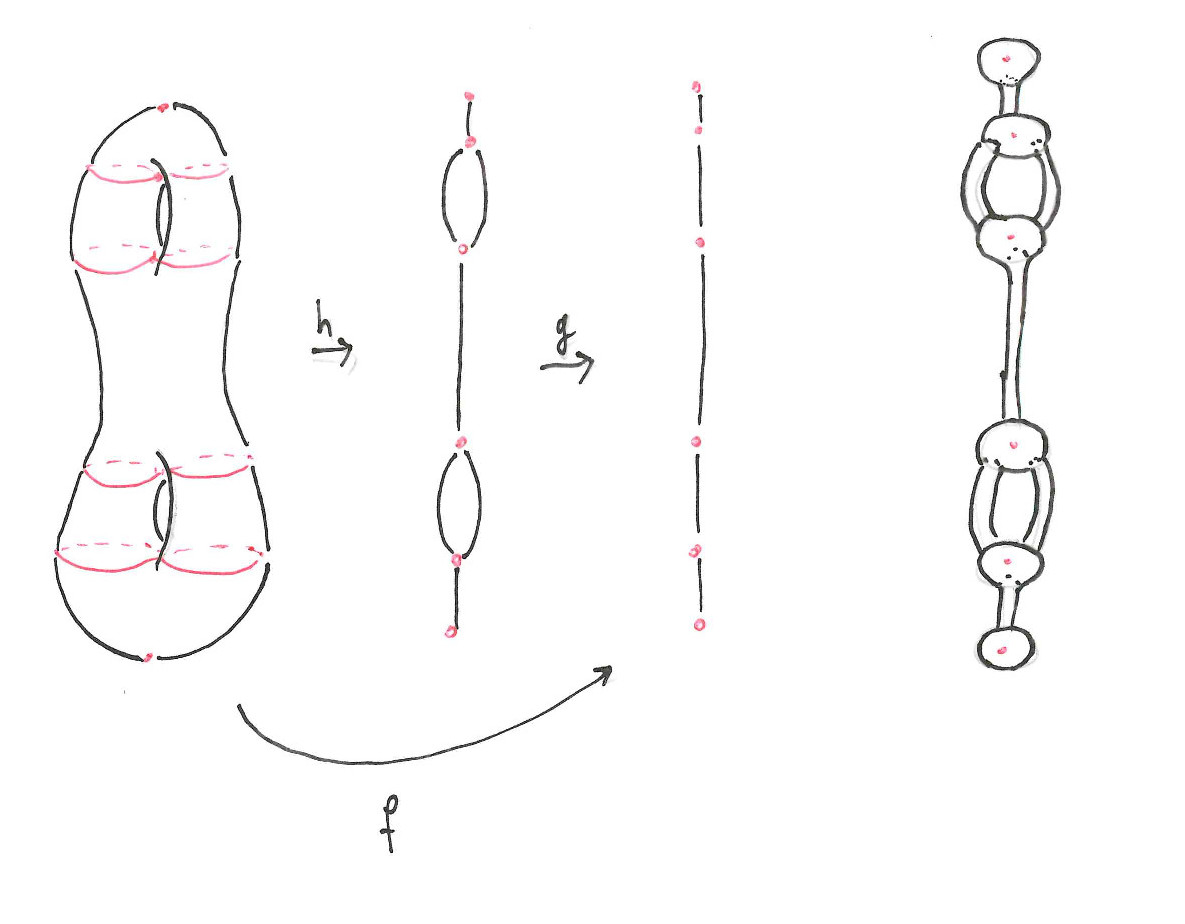
\includegraphics[height=4in]{figures/typicalmorse.jpg}
	\label{fig:typicalmorse}
\end{figure}

\begin{proof}
	Figure \ref{fig:typicalmorse} depicts a typical Morse function acting on the closed oriented surface of genus 2, and samples some of the notation we will define initially.
	We begin by examining the preimages of points $x\in\R$.
	Denote the space $f\inv(x)$ by $\Sigma_x$, a small interval around $x$ by $\varepsilon(x)=(x-\varepsilon,x+\varepsilon)$, and the neighbourhood in $\Sigma$ around $\Sigma_x$ by $f\inv(\varepsilon(x))=\varepsilon(\Sigma_x)$.
	The spaces $\Sigma_x$ and $\varepsilon(\Sigma_x)$ may not be connected, so we index the connected components by superscript.
	Let $p$ be a critical point of $f$ with critical value $f(p)=x$.
	By our assumption that critical values are distinct, $p$ is the only critical point of $f$ in $\Sigma_x$.
	The connected component of $\Sigma_x$ containing $p$ is called the \emph{singular fiber} at $p$ and is denoted $\Sigma_x^p$.
	The connected component of $\varepsilon(\Sigma_x)$ containing $p$ is called the \emph{critical neighbourhood} at $p$ and is denoted $\varepsilon^p(\Sigma_x)$.
	By the regular value theorem, any regular value pulls back through $f\inv$ to a disjoint collection of circles in $\Sigma$ called \emph{regular fibers}.
	Likewise, a neighbourhood $\varepsilon(x)$ that contains no critical values of $f$ pulls back to a disjoint collection of annuli in $\Sigma$.
	The restriction of $f$ to the components of $\Sigma_x$ that do not contain a critical point has $x$ as a regular value, so the remaining connected components of $\Sigma_x$ are all copies of $S^1$ that we index by $\Sigma_x^i$ for $i=1,\dots,k$, and their associated neighbourhoods are the annuli $\varepsilon^i(\Sigma_x)$.
	When referring to an arbitrary connected subspace of $\Sigma_x$ that could be the singular fiber $\Sigma_x^p$ or a regular fiber $\Sigma_x^i$, we will use the notation $\Sigma_x^*$.
	
	The shape of a singular fiber $\Sigma_x^p$ is determined by the index of $p$.
	Because $f$ is a Morse function whose domain is a surface, its critical points are easily classified by the Morse lemma (Lemma \ref{lem:morselemma}).
	Locally in $\Sigma$, a critical point of index 0 is a minimum, of index 1 a saddle, and of index 2 a maximum of $f$.
	
	Let $x$ be a critical value for the critical point $p$ and take $\varepsilon$ to be small enough that $\varepsilon(x)$ contains no critical values other than $x$.
	When $p$ is of index 0 or 2, we can immediately deduce that $\varepsilon^p(\Sigma_x)$ is diffeomorphic to a disc.
	When $p$ is of index 1, the Morse lemma tells us that $\Sigma$ looks like a standard saddle near $p$.
	The intersection of $\Sigma_x^p$ with this saddle is a cross whose centre is $p$.
	For $y\in\varepsilon(x)$, $y$ is a regular value whose preimage is a disjoint union of circles.
	The circles above and below the saddle singularity are the result of smoothing out the cross into a pair of oriented arcs, done in two possible ways.
	The orientations of these circles orient the cross, which has two incoming arms and two outgoing arms which appear in alternating order.
	A Morse function has distinct singular fibers, so the cross we know about in $\Sigma_x^p$ must have its arms connected in $\Sigma_x^p$ through nonsingular orientation--preserving arcs.
	We can then see that $\Sigma_x^p$ is a figure 8, and $\varepsilon^p(\Sigma_x)$ is a pair of pants in $\Sigma$.
	

	\begin{figure}
		\centering
		\caption{Smoothing a cross into a saddle}
		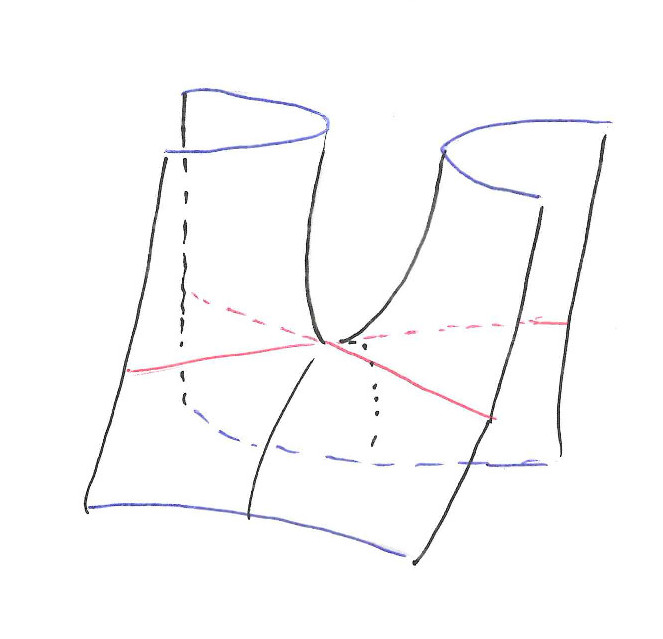
\includegraphics[height=3in]{figures/smoothcross.jpg}
		\label{fig:smoothcross}
	\end{figure}
	
	This analysis is sufficient to form a handle decomposition for a cobordism of $(\Sigma,\emptyset)$.
	We begin with the 3--manifold $\Sigma\times\I$ with boundary components $\Sigma_0=\Sigma\times\{0\}$ and $\Sigma_1=\Sigma\times\{1\}$, and let $f:\Sigma_0\to\I$ be a Morse function with distinct critical values $x_i$.
	The general idea is that we attach handles to $\Sigma_0$, altering that boundary component until it is empty.
	The $x_i$ partition $\I$ into open intervals containing only regular values.
	We take the associated regular annuli to be attaching regions for 3--dimensional 2--handles, and then fill in what remains with 3--dimensional 3--handles.
	
	For an interval $(x_i,x_{i+1})$, consider the subinterval $\varepsilon(t_i)$ where $x_i<t_i<x_{i+1}$ and $\varepsilon$ is small enough that $\varepsilon(t_i)$ contains neither $x_i$ nor $x_{i+1}$.
	Take the associated regular annuli $\varepsilon(\Sigma_{t_i})$ to be the attaching regions for 3--dimensional 2--handles.
	The boundary component that was once $\Sigma_0$ is now the result of removing the interiors of the annuli $\varepsilon(\Sigma_{t_i})$ from $\Sigma_0$ for each $t_i$, and then introducting discs parallel to the cores of the attached 2--handles.
	These discs are seen as $\DD\times\{0\}$ and $\DD\times\{1\}$ inside of a 2--handle $\DD\times\D^1$.
	The boundary circles of the discs are $\Sigma_{t_i-\varepsilon}$ and $\Sigma_{t_i+\varepsilon}$ for each $i$.
	
	There are now intervals about each critical point that we know, from our analysis above, pull back to discs, annuli, and pairs of pants.
	Each of these subsurfaces have circle boundaries that correspond to the regular fibers $\Sigma_{t_i-\varepsilon}$ and $\Sigma_{t_i+\varepsilon}$ which were capped with discs in the previous step.
	The altered boundary described before is therefore a collection of copies of $S^2$, which we take to be the attaching regions of 3--dimensional 3--handles.
	
	With these handles attached, we obtain $(\Sigma\times\I)\cup\{\textrm{2--handles}\}\cup\{\textrm{3--handles}\}$, which is a 3--manifold with exactly one boundary component of $\Sigma_1$, i.e. a cobordism of the pair $(\Sigma,\emptyset)$.
	
	The corresponding dual handle decomposition is realized by turning the process upside down.
	Where we previously had 3--handle attachments with cores $\D^3\times\{\vec{0}\}$ and cocores $\{\vec{0}\}\times\{\vec{0}\}$, we now have 0--handles with cores $\{\vec{0}\}\times\{\vec{0}\}$ and cocores $\D^3\times\{\vec{0}\}$.
	In other words, the dual construction begins by taking the disjoint union of a collection of 3--discs that correspond to the space obtained by capping the boundary circles of the components $\varepsilon(\Sigma_{x_i})$ with 2--discs and then filling the spheres with 3--balls.
	Where we previously had 2--handle attachments with cores $\DD\times\{\vec{0}\}$ and cocores $\{\vec{0}\}\times\D^1$, we now have 1--handle attachments with cores $\{\vec{0}\}\times\D^1$ and cocores $\DD\times\{\vec{0}\}$.
	In other words, we connect the 0--handles together using 1--handles.
	The old belt 0--spheres of the 2--handles in the previous construction correspond here to new attaching 0--spheres, and the attaching maps are chosen to preserve orientability cf.\ Remark~\ref{rmk:1handle}.
	The new attaching 0--spheres bound the new cores, the old core 2--discs are now cocores.
	This construction yields a 3--manifold whose boundary is exactly $\Sigma$, and is indeed another cobordism of the pair $(\Sigma,\emptyset)$.
	
	A Stein factorization $f=g\comp h$ is simple to describe.
	Define the equivalence relation $\sim$ on the points in $\Sigma$ by putting $p\sim q$ if and only if $f(p)=f(q)=x$ and $p$ and $q$ are in the same subspace $\Sigma_x^*$.
	Then $h$ is the quotient map $\Sigma\to \Sigma/\!\!\sim$ where the points of $\Sigma/\!\!\sim$ are the subspaces $\Sigma_x^*$, and $g$ is the map $\Sigma/\!\!\sim\, \to\R$ defined by $g(\Sigma_x^*)=x$.

	The Stein complex $S=\Sigma/\!\!\sim$ can be viewed as a graph $G$.
	A critical value $x=f(p)$ has an associated singular fiber $\Sigma_x^p$ in $S$, and possibly some copies of $S^1$ given by $\Sigma_x^i$.
	We take the associated points $h(\Sigma_x)$ in $S$ for each critical value to be the vertex set $v(G)$.
	For a pair of adjacent critical values $x_{j}$, $x_{j+1}$, an appropriate choice of $\varepsilon$ and $x\in(x_{j},x_{j+1})$ yields a collection of regular annuli $\varepsilon(\Sigma_x)$ in $\Sigma$ that has boundary inside of $\Sigma_{x_{j}}\cup\Sigma_{x_{j+1}}$.
	In $S$, we find $h(\varepsilon(\Sigma_x))$ to consist of 1--dimensional strands that connect components of $\Sigma_{x_{j}}$ and $\Sigma_{x_{j+1}}$.
	The set of pairs $(v,w)$ of connected subspaces with $v\in\Sigma_{x_{j}}$ and $w\in\Sigma_{x_{j+1}}$ such that $v$ and $w$ are connected by a strand in $S$ forms the edge set $e(G)$.
	
	At this point, $G$ corresponds exactly to the dual handle decomposition given earlier.
	For each vertex of $G$ we get a 0--handle.
	For each edge, a 1--handle.
	We attach 1--handles with only one demand: that the resulting space continues to be orientable.
\end{proof}

The Stein complex obtained in the proof of Theorem~\ref{thm:2bound3} may have superfluous vertices.
In particular, a vertex $v$ of $G$ that is adjacent to exactly two verticex $u$ and $w$ via the edges $(u,v)$ and $(v,w)$ may be replaced, along with its adjacent edges, by a single edge $(u,w)$.
To see that the handle decomposition described by this Stein complex graph is equivalent, examine the attaching region of the 1--handle corresponding to $(u,v)$ as it sits inside the boundary of the 0--handle corresponding to $v$.
This region may be isotoped over the 1--handle corresponding to $(v,w)$, where it ends up in the boundary of the 0--handle corresponding to $w$.
We are left with a 0--handle $v$ and 1--handle $(v,w)$ that are contractible into $w$.

\section{3--Manifolds Bound 4--Manifolds}
\label{sec:3bound4}

To extend the results of the previous section to the case of 3--manifolds bounding 4--manifolds, we consider generic proper smooth maps from closed orientable 3--manifolds into the 2--ball $B^2$.
Such a map is Morse--like in the sense that its singular set is well behaved, it can be studied via the same techniques as in Section \ref{sec:2bound3}, and we may recover a Stein factorization and Stein complex that define a handle decomposition for a bounding 4--manifold.

\begin{theorem}
	\label{thm:3bound4}
	Let $M$ be a closed orientable 3--manifold.
	Then a proper generic smooth map $f:M\to \BB$ determines a handle decomposition for a cobordism of the pair $(M,\emptyset)$.
\end{theorem}

\begin{proof}
	By Sard's theorem, the image of the singular set $f(s_f)$ in $\BB$ has Lebesgue measure 0.
	By genericity, and because the maps constructed in Chapter \ref{cha:alg1} satisfy this requirement, we take $s_f$ to consist of a set of arcs in the plane that intersect each other only pairwise and transversally, in such a way that $\BB\setminus s_f$ consists of a collection of regions $R_i$ homeomorphic to copies of $\BB$ along with a single annular region $R_\infty$ that does not intersect $f(M)$, and in such a way that $f(s_f)$ has a natural structure as a simple undirected 4--valent planar graph.
	We classify the critical values of $f$ as codimension 1 inside of arcs away from crossings, and codimension 2 at arc crossings.
	This classification makes the simple undirected planar graph structure of $f(s_f)$ explicit.
	The vertex set is given by the set of codimension 2 critical values and the edge set is the collection of codimension 1 critical values.
	
	We obtain a 4--manifold with boundary $M$ by attaching 2--handles corresponding to the regular regions $R_i$, 3--handles corresponding to codimension 1 singularities, and 4--handles corresponding to codimension 2 singularities.
	
	We will first focus on a region $R$ in $\BB$ that is not $R_\infty$.
	Begin by ``shrinking'' $R$ away from $f(s_f)$ into a space $\D$ that is homeomorphic to $\DD$
	Every point of $\D$ has preimage a disjoint collection of circles by the regular value theorem, so we centre our analysis on an arbitrary regular value $x$ and its regular fibers, where $M_{x,k}$ denotes the $k\nth$ regular fiber mapped over $x$ by $f$.
	An appropriate closed tubular neighbourhood of $M_{x,k}$ will consist entirely of regular fibers that map into $\D$ and has the structure of a closed 2--disc bundle over the circle, hence is a solid torus.
	The neighbourhood can be extended to enclose the entirety of $f\inv(\D)$.
	
	In summary, an arbitrary point $x_i$ is chosen from a closed 2--disc $D_i$ which itself is taken as a shrinking of an open region $R_i$.
	For each $k$, the $k\nth$ regular fiber $M_{i,k}$ over $x_i$ is taken as the zero section of a 2--disc bundle that maps over $D_i$.
	Such a bundle is an open solid torus, and the $k\nth$ bundle is denoted $V_{i,k}$.
	Of particular importance in $V_{i,k}$ are the zero section and a certain isotopy class of longitudes.
	The zero section $z(V_{i,k})$ is a regular fiber that maps over a point interior to $\D_i$, and the longitudinal isotopy class is the one that contains regular fibers that map to single boundary points of $D_i$.
	This pair determines an attaching map for 4--dimensional 2--handle attached over $V_{i,k}$.
	
	\begin{figure}
		\centering
		\captionsetup{justification=centering}
		\caption{Closed sleeve around an arc of codimension 1 critical values and the two neighbouring codimension 2 critical values}
		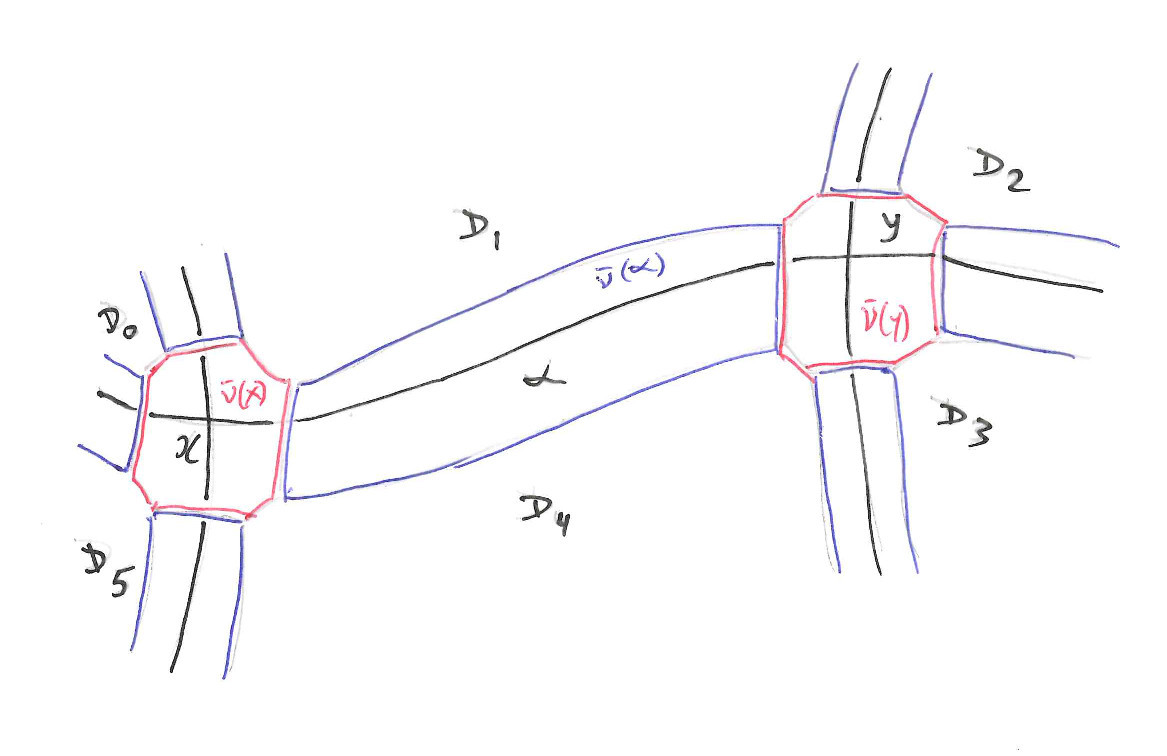
\includegraphics[height=4in]{figures/critsleeve.jpg}
		\label{fig:critsleeve}
	\end{figure}
	
	Consider an arc $\alpha$ of codimension 1 critical values that separates a pair of regions $R_i$ and $R_j$ where either $i$ or $j$ may be $\infty$.
	As when we considered regions, $\alpha$ has been shrunk away from the codimension 2 critical values it connects.
	Let $\nbhd{\alpha}$ be a closed ``sleeve'' around $\alpha$ whose boundary intersects the boundaries of $D_i$ and $D_j$ as in Figure \ref{fig:critsleeve}.
	The restriction of $f$ to the preimage of a linear transversal to $\alpha$ that connects $D_i$ and $D_j$ is, itself, a Morse function.
	The intersection with $\alpha$ is a critical point of this restriction, and the same techniques from the proof of Theorem \ref{thm:2bound3} may be applied to $f\inv(\nbhd{\alpha})$.
	A strand of singular fibers over $\alpha$ consists of an interval in the case of an extremum for the associated Morse function or an interval crossed with the figure 8 when the associated Morse function yields a saddle singularity.
	The critical neighbourhood $f\inv(\nbhd{\alpha})$ contains a connected component that is either $\DD\times\I$ when we have cross sectional extremum, or $P\times\I$, where $P$ is the pair of pants surface, i.e.\ the 2--sphere with three interior 2--balls removed, when the cross section yields a saddle.
	All remaining connected components are intervals crossed with regular annuli.
	We use $A=S^1\times\D^1$, alternatively the 2--sphere with two interior 2--balls removed, to denote an annulus, and find $A\times\I$ to be the form of all remaining connected components.
	
	Whenever one of the regions that $\alpha$ separates is $R_\infty$, the cross section necessarily gives us an extremum, and the critical neighbourhood over $\nbhd{\alpha}$ is $\DD\times\I$.
	We call $\alpha$ a \emph{definite fold} when the critical neighbourhood is $\DD\times\I$, and an \emph{indefinite fold} when the critical neighbourhood is $P\times\I$.
	
	Let $x$ be a codimension 2 critical value and $\nbhd{x}$ the closed neighbourhoods whose boundary agrees with the shrunken regions and arc sleeves it is near as in Figure \ref{fig:critsleeve}.
	The possible singular fibers over $x$ are cataloged in \cite{Saeki}, and Figure \ref{fig:saekising} displays them.
	The singular fibers over $x$ may be disconnected.
	When that is the case, the fibers have the form seen in our codimension 1 analysis.
	Otherwise, the singular fiber has the shape of a 4--valent directed graph.
	The regular fibers are still copies of $S^1$.
	In each case $f\inv(\nbhd{x})$ is a 3--dimensional thickening of the corresponding fibers, hence is a disjoint collection of handlebodies of genus 0,1,2, or 3.
	The neighbourhood of a regular fiber is still a solid torus, so all but at most two of the connected components of $f\inv(\nbhd{x})$ will be genus 1 handlebodies.
	
	\begin{figure}
		\centering
		\captionsetup{justification=centering}
		\caption{Possible singular fibers of a proper generic smooth map from an orientable 3--manifold to a surface}
		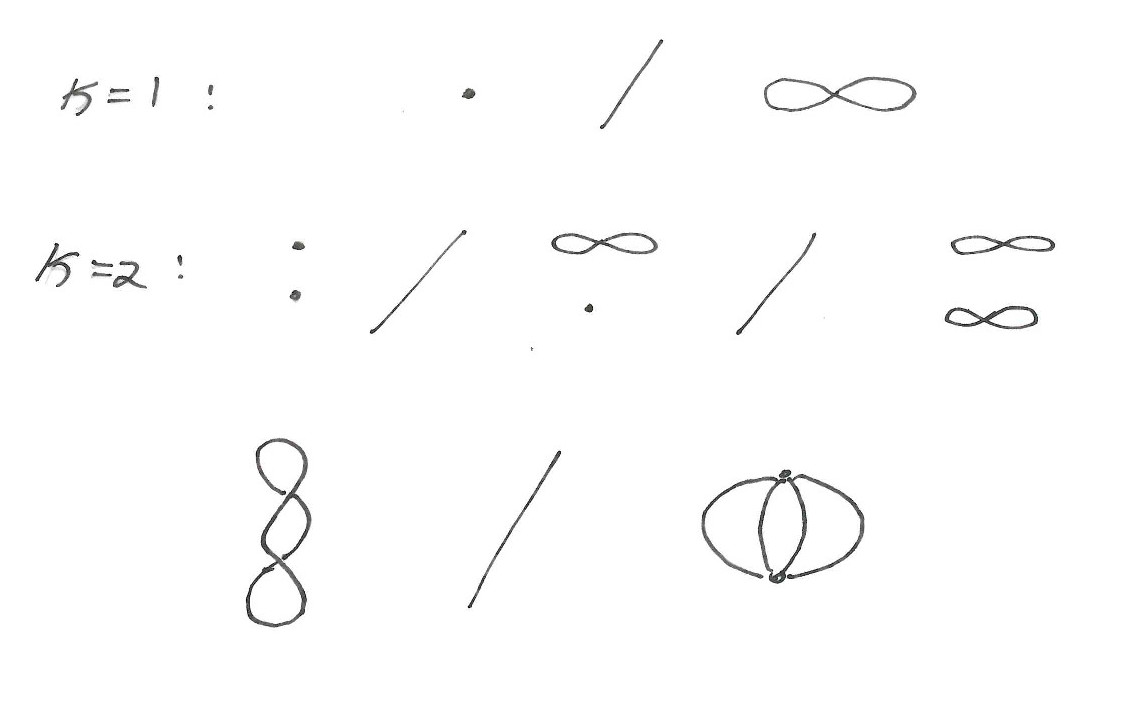
\includegraphics[height=3in]{figures/saekising.jpg}
		\label{fig:saekising}
	\end{figure}
	
	We may now begin describing a handle decomposition for a cobordism $W$ of the pair $(M,\emptyset)$.
	Begin with $M\times\I$, whose boundary is $M_0\sqcup M_1$ with $M_0=M\times\{0\}$ and $M_1 = M\times\{1\}$, and a proper generic smooth map $f:M_0\to\BB$.

	For each $i<\infty$ indexing the connected regions of $\BB\setminus f(s_f)$, we index over $k$ the connected components of $f\inv(R_i)$.
	Consider $D_i\subset R_i$, a 2--disc of regular values, and $V_{i,k}$, the $k\nth$ regular solid torus that maps over $D_i$.
	The solid torus $V_{i,k}$ has a trivial disc bundle structure over the regular fiber $M_{i,k}=z(V_{i,k})$, and $f(M_{i,k})=x$ in the interior of $\D_i$.
	Because we consider a single solid torus for the rest of this argument, we abbreviate $V_{i,k}$ to $V$, $M_{i,k}$ to $z(V)$ and $\D_i$ to $\D$.

	Let's remember what we're doing here --- we're attaching handles in such a way that, once all handles have been attached, the boundary component $M_0$ of $M\times\I$ has been filled in.
	In this step we attach 2--handles over $V$.
	Our goal is to do so in such a way that we remove the ``bad'' solid torus $V$ and replace it with a solid torus that is ``nice,'' where ``nice'' means that the newly introduced solid torus can be filled in by attaching 3-- and 4--handles.
	This happens by deleting $V$ and gluing 2--discs to the longitudes in $\pd V$ that are regular fibers of points in the boundary of $D$.
	To attach a 2--handle over $V$, we need
	\begin{enumerate}
		\item The isotopy class of an embedding $g:S^1\to M_0$, and
		\item the isotopy class of an identification $G:S^1\times\DD\to\nbhd{g(S^1)}$.
	\end{enumerate}
	The embedding $S^1\to M_0$ is easy enough to define as we will just be identifying $S^1$ with $z(V)$.
	This $S^1$ lives as the attaching sphere $S^1\times\{0\}$ inside of the 2--handle $\DD\times\DD$ that we plan to attach.
	Taking $\pd (\DD\times\DD)=(S^1\times\DD)\cup(\DD\times S^1)$ to be the genus 1 Heegard splitting of $S^3$, we will be defining a map $G:V\to S^1\times\DD$, where $S^1\times\DD$ is the first torus component.
	We call the other torus $V^*$.
	In order to satisfy our desired criteria, we need to have $G$ be in the isotopy class of a map that takes a regular fiber $J$ over a point in the boundary of $\D$ to $S^1\times\{1\}$.
	When this is true, we may form the adjunction $(M\times\I)\cup_{G\inv}(\DD\times\DD)$ and $J$ bounds a disc in $V^*$.
	Every fiber in the interior of $V$ now bounds a disc, and the new boundary is exactly $V^*$, whose meridians are the fibers that project over the boundary of $\D$.
	This is the property we wanted --- we've replaced the ``bad'' solid torus $V$ with the ``nice'' solid torus $V^*$.
	
	\begin{figure}
		\centering
		\captionsetup{justification=centering}
		\caption{The solid tori $V$ and $V^*$ with boundary curves $J$, $K$, and $L$.}
		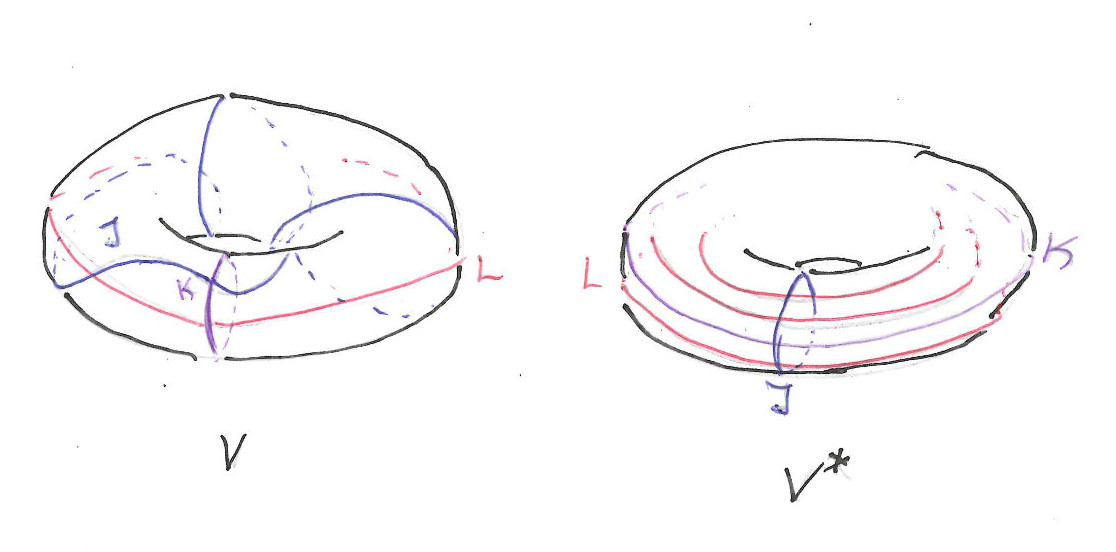
\includegraphics[width=6in]{figures/VV.jpg}
		\label{fig:VV*}
	\end{figure}
	
	A class $[G]$ satisfying the above is unique and it exists.
	To see why, let $\varphi:V\to S^1\times\DD$ be any trivialization of $V$, take $K=\varphi\inv(\{1\}\times S^1)$ to represent the meridinal isotopy class of $V$, and take $L$ be the longitude in $\pd V$ defined by $L=\varphi\inv(S^1\times\{1\})$.
	Let $J=f\inv(q)$ in $\pd V$ represent the isotopy class of regular fibers over boundary points of $\D$, where $q$ is an arbitrary point in the boundary of $D$.	
	Figure \ref{fig:VV*} shows the curves $J$, $K$, and $L$ with orientations sitting on $\varphi(V)$.
	Thinking of $S^1\times\DD$ as a subset of $\C^2$ gives it a natural orientation, which we have pulled back through $\varphi$ onto $K$ and $L$.
	We give $J$ a compatible orientation so that its intersections with $K$ and $L$ can be counted.
	Put $\kappa$ to be the oriented intersection number of $J$ and $L$.
	Then $\varphi(J)\in \pd\varphi(V)$ is in the isotopy class of $h_M^{\kappa}(\varphi(L))$, where $h_M$ is the meridinal twist defined in Theorem \ref{thm:mpgV}.
	Take $G=H_M^{-\kappa}\comp\varphi$, where $H_M$ is the extension of $h_M$ to the solid torus defined in Remark \ref{rmk:2handle}.
	In the boundary of $G(V)$, $G(J)$ is in the isotopy class of $S^1\times\{1\}$, $G(K)$ is in the isotopy class of $\{1\}\times S^1$, and $G(L)=h_M^\kappa(S^1\times\{1\})$.
	Existence of $G$ is shown, and uniqueness up to isotopy comes from the same uniqueness in trivializations of $V$ and of $H_M$.
		
	With 2--handles attached, we move onto the preimages of arc sleeves.
	Let $\nbhd{\alpha}$ be an arc sleeve, and consider the connected components of $f\inv(\nbhd{\alpha})$.
	Figure \ref{fig:arcsleevepre} displays the possible connected components of arc sleeve preimages, each of which has the form of a surface crossed with the interval.
	The boundary circles of these surfaces at a cross section $\Sigma\times\{t\}$ project through $f$ over the boundaries of shrunken regions, so they are filled with discs that sit inside of attached 2--handles from the previous step.
	In each case, we obtain a copy of $S^2\times\D^1$ over which we attach a 3--handle.
	The further modification to $M_0$ that takes place when we attach 3--handles can be thought of as the deletion of a copy of $S^2\times D^1$ followed by gluing 3--discs over the newly created 2--sphere boundary components.
	
	\begin{figure}
		\centering
		\captionsetup{justification=centering}
		\caption{Possible connected components of arc sleeve preimages}
		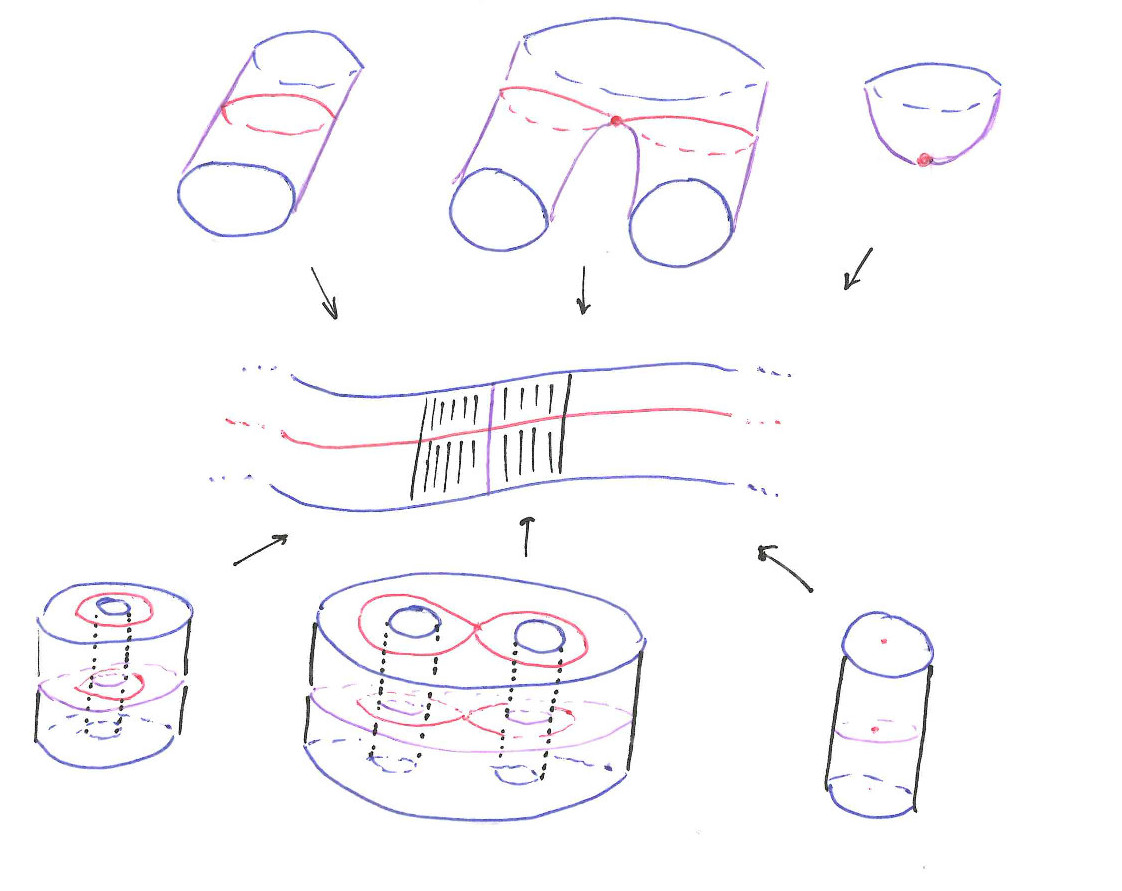
\includegraphics[height=4in]{figures/arcsleevepre.jpg}
		\label{fig:arcsleevepre}
	\end{figure}
	
	Finally, let $x$ be a codimension 2 critical value and let $\nbhd{x}$ be its sleeve.
	We find $x$ at the crossing of a pair of strands of codimension 1 critical values, and those strands are classified as definite or indefinite folds.
	The analysis of the codimension 2 critical value is then broken down into five cases.
	In four cases, we are able to extend the codimension 1 situation.
	This happens when the singular fiber is disconnected, called an \emph{uninteractive} singular fiber, or when one of crossing folds is definite.
	When both folds are indefinite and the singular fiber is connected, then the singular fiber is called \emph{interactive} and we defer to the analysis in \cite{CostThur08}.
	
	First we look at the connected components of $f\inv(\nbhd{x})$ that do not contain a singular fiber over $x$.
	These connected components are made from regular fibers, i.e.\ circles, that project over $\nbhd{x}$, i.e. a 2--disc.
	As in the case of regions of regular values, they are solid tori $V_{x,k}$, using the same naming convention that has been established for solid tori that map over the regions $D_i$.
	Seeing $V_{x,k}$ as a 2--disc bundle over $f\inv(x)$, we can find an isotopy class of longitudes that project over single points in the boundary $\pd\nbhd{x}$.
	These longitudes bound discs introduced during 2-- and 3--handle attachment.
	The union of all such discs yields a solid torus $V_{x,k}^*$ in the boundary.
	The boundary component consisting of $V_{x,k}$ and $V_{x,k}^*$ is described by the Heegaard splitting $V_{x,k}\cup_\varphi V_{x,k}^*$ where $\varphi$ takes a longitude of $V_{x,k}$ to a meridian of $V_{x,k}^*$.
	This is the standard genus 1 Heegaard splitting of $S^3$, so we have a copy of $S^3\times\D^0$ over which we may attach a 4--handle.

	The component that comes from an uninteractive definite fold is of the form $\DD\times\I$ as in the case of codimension 1 critical values.
	The 2--sphere boundary of this shape is filled with 2--discs from our 2-- and 3--handles, so this shape is the adjunction of a pair of 3--discs glued over their boundary.
	This is the genus 0 Heegaard splitting of $S^3$, so we have a copy of $S^3\times\D^0$ over which we may attach a 4--handle.
		
	\begin{figure}
		\centering
		\caption{Destabilizing pairs for the pair of pants}
		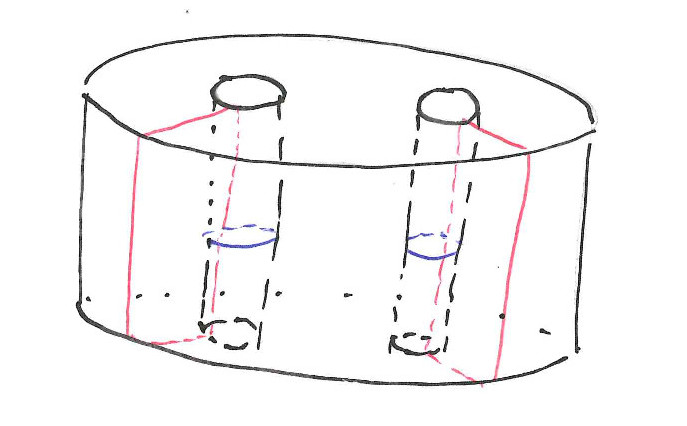
\includegraphics[height=3in]{figures/destabpants.jpg}
		\label{fig:destabpants}
	\end{figure}
		
	An uninteractive singular fiber that comes from an indefinite fold is the figure 8, and the preimage $f\inv(\nbhd{x})$ is a closed tubular neighbourhood of the figure 8 graph, which is homeomorphic to the pair of pants crossed with an interval.
	Here, we find a Heegaard splitting of genus 2 with two destabilizing pairs, showing that the splitting is a splitting of $S^3$, and we can attach a 4--handle to it by Theorem \ref{thm:lilwald}.
	An appropriate choice of meridians in $f\inv(\nbhd{x})$ would be a pair of curves that run from cuff to waist along the inside of each of the legs in the pair of pants, crest the waist, then down the outside of the legs back to the cuff.
	Meridians for the solid filled by our 2-- and 3--handles would run around the cuffs of each leg.
	Figure \ref{fig:destabpants} illustrates the idea.
	
	When an indefinite and definite fold interact, we get the same shapes found in the case of an uninteractive definite fold.
	From a 1--dimensional Morse function viewpoint, we witness a homotopy of a pair of peaks separated by a saddle come together into a single peak, eliminating the saddle.
		
	This leaves us with the case of interacting indefinite folds.
	The full analysis is covered in Section 4.4 of \cite{CostThur08}.
	They show that filling in $f\inv(\pd\,\nbhd{x})$ with 2--discs and gluing the two genus 3 handlebodies together over $f\inv(\pd\,\nbhd{x})$ results in a Heegard splitting of $S^3$ by explicitly finding 3 destabilizing pairs.
	We attach 4--handles over these 3--spheres.
	Attaching a 4--handle over a 3--sphere fills in the 3--sphere with a 4--disc, so these final modifications completely eliminate what is left of $M_0$.
	We are left with a handle decomposition for a cobordism of the pair $(M,\emptyset)$ built on top of $M_0$ in $M\times\I$.
\end{proof}

Let $f:M:\to\BB$ be a proper generic smooth function and $W$ a the cobordism of the pair $(M,\emptyset)$, both as per the construction in Theorem \ref{thm:3bound4}. 
Because the handle decomposition produced for $W$ consists of handles of index 2,3, and 4, the associated dual decomposition contains handles of degree 0,1, and 2.
Our goal is to obtain a combinatorial description of this decomposition, and we find this through the Stein complex.

Recall that the Stein complex for a Morse function on a surface was given by a 1--complex.
In the case of a proper generic smooth map $M\to\BB$, the Stein complex is given by a 2--complex $S$.
The vertices of $S$ correspond to 0--handles, the edges to 1--handles and the 2--cells to 2--handles.

We define the Stein factorization and complex of $f$ as usual.
Let $\sim$ be an equivalence relation on $M$ defined by $p\sim q$ if and only if $f(p)=f(q)=x$ and $p$, $q$ are in the same connected component of $f\inv(x)$.
Then $f=g\comp h$ where $h$ is the quotient map $M\to M/\!\!\sim$ and $g$ takes a point in $f\inv(x)$ to $x$.

\begin{theorem}
	\label{thm:stein2complex}
	Let $f$, $M$, $S$, and $W$ be as we defined above.
	Then $S$ is a 2--dimensional CW--complex that embeds flatly in $W$.
\end{theorem}

\begin{proof}
	There are only a few locations where $S$ could fail to be a CW--complex, and those are found over the critical values of $f$.
	We construct $S$ as we would any other CW--complex, by iteratively attaching cells of increasing dimension, and define a map $\varphi:S\into W$ that is almost a flat embedding in a similar fashion.
	Let $S$ be empty and begin by adding 0--cells to $S$.
	
	For a codimension 2 singular value $x$ of $f$, the fibers of over $x$ were discussed in Theorem \ref{thm:3bound4}.
	The Stein factorization $f=g\comp h$ has $h$ crush each fiber to a point, which we take as a new 0--cell in $S$.
	Let $\nbhd{x}$ be a sleeve of $x$ as in Theorem \ref{thm:3bound4}.
	In the construction of $W$, we attached 4--handles over 3--spheres with Heegaard decompositions over $f\inv(\nbhd{x})$.
	The cocore of a 4--handle is a single point, so we associate the 0--cells of $S$ with the cocores of 4--handles in $W$.
	Let $x_i$ be a fiber over $x$, let $H_i^4\subset W$ be the 4--handle associated to $x_i$, let $c_i\in H_i^4$ be the cocore of $H_i^4$, and let $v_i$ be the vertex of $S$ associated to $x_i$.
	Define $\varphi(v_i)=c_i$.
	
	We can now add edges to $S$.
	Let $\alpha$ be an open strand of codimension 1 critical points of $f$ with $\pd\overline\alpha=\{x,y\}$, a pair of codimension 2 critical points of $f$.
	Pulling back $\alpha$ to $M$ yields an open interval crossed with the fibers over any point of $\alpha$ and pulling back $\overline\alpha$ connects the fibers over $x$ and $y$.
	For a fiber $\alpha_i$ over $\alpha$ with endpoints $\alpha_i^x$ sitting inside of a fiber over $x$ and $\alpha_i^y$ sitting in a fiber over $y$, we add an edge attached over the vertices $v_i^x$ and $v_i^y$ associated to the fibers over $x$ and $y$.
	This corresponds to the action of $h$ on $\alpha_i$, which crushes the interval of fibers to an interval.
	
	Let $\nbhd{\alpha}$ be a sleeve of $\alpha$ as in Theorem \ref{thm:3bound4}.
	To construct $W$ we attached 3--handles over copies of $S^2\times\D^1$, those $S^2\times\D^1$ contained copies of $\Sigma\times\D^1$ with $\Sigma$ the 2--sphere with one, two, or three open 2--balls removed, and those $\Sigma\times\D^1$ projected over $\nbhd{\alpha}$.
	The cocore of a 3--handle is a copy of $\D^1$, which corresponds to an edge in $S$.
	Let $\alpha_i$ be a fiber over $\alpha$, $H_i^3$ the 3--handle associated with $\alpha_i$, $c_i$ the interval cocore of $H_i^3$, and $e_i$ the edge of $S$ corresponding to $\alpha_i$ with $\pd e_i=\{u,v\}$.
	Because $e_i$ is a 1--cell, it is homeomorphic to an interval $[\,0,1\,]$, so we take a slightly smaller closed subinterval $e_i'$ in $e_i$ (just as we can take $[\,\varepsilon,1-\varepsilon\,]$ inside of $[\,0,1\,]$) and define $\varphi(e_i')=c_i$.
	The endpoints of $c_i$ are the belt sphere of $H_i^3$, and they intersect the 4--handles $H_u^4$ and $H_v^4$ corresponding to $u$ and $v$.
	The intersection points are in the boundary 3--spheres of these 4--handles, so there are straight lines inside of the 4--handle that connect the cocore to these boundary points.
	Define $\varphi$ on $e_i\setminus e_i'$ to be those straight line segments in the appropriate continuous way.
	
	And finally, the 2--cells.
	Let $R$ be an open ball of regular values in the plane, and let $D$ be the 2--disc inside of $R$ that pulls back through $f$ to a disjoint collection of solid tori over which we attached 2--handles in our construction of $W$.
	Let $H$ be the 2--handle attached over a solid torus $V$ projecting over $D$.
	The boundary of $H^2$ is a 3--sphere with genus 1 Heegaard splitting consisting of $V$ and a dual torus $V^*$.
	We attached $H^2$ because we wanted to fill the boundary of $V$ with 2--discs that were easy to attach 4-- and 3--handles over, and $V^*$ is also contained in the union of these 4-- and 3--handles.
	The vertices and edges of $S$ corresponding to this collection 4-- and 3--handles forms a cycle $C$ in the 1---skeleton of the Stein complex already built.
	We know that $R$ contains only regular values, so it pulls back to a disjoint collection of open solid tori.
	Let $U$ be the open solid torus in this collection with $f(U)=R$ and $V\subset U$.
	In particular, $\pd V=\pd V^*\subset U$.
	The fibers of $S$ are fibers of $f$ that project over the regular values in $R$, so $h(U)$ is a 2--ball.
	The closure of $U$ intersects the singular fibers corresponding to the 4-- and 3--handles that contain $V^*$.
	We take $h(U)$ in $S$ to be a 2--cell attached over $C$.

	To define $\varphi$ on the 2--cell $\sigma_U$ corresponding to $U$, we start by defining it on $\sigma_V$, a subdisc of $\sigma_U$ (cf.\ the case of defining $\varphi$ on the edges of $S$, where $\sigma_V\subset\sigma_U$ just like how $\{z\in\C:|z|^2\leq 1-\varepsilon\}\subset\DD$).
	Recall that	$H^2$ is the 2--handle attached over $V$.
	It is useful to think of $H^2$ as a $\DD$ bundle over $\DD$, where the base space and zero section are the cocore $C_V$ of $H^2$.
	We define $\varphi(\sigma_V)=C_V$, and then examine the intersection of $C_V$ with the 4-- and 3--handles of $W$.
	The collection of higher index handles that intersect $H^2$ is exactly the collection that contains $V^*$, and the intersection is exactly $V^*$.
	The cocore $C_V$ intersects $V^*$ in exactly the belt sphere of $H^2$.
	We then extend $\varphi$ to $\sigma_U\setminus\sigma_V$ exactly as we did with the edges of $S$, by connecting the belt sphere of $H^2$ with the cocores of the 4-- and 3--handles by line segments.
	
	This demonstrates first that the Stein complex $S=h(M)$ has the structure of a 2--complex.
	Secondly, the map $\varphi:S\into W$ constructed here is piecewise--linear where it is not smooth, so can be smoothed into a flat embedding of a CW--complex.											
\end{proof}

In Section \ref{sec:proj} it is convenient to remove open balls from a given 3--manifold $M$ and build a projection of $M'$ instead.
We want the results of this section to still apply, so we state this in Theorem \ref{lem:stillworks}

\begin{lem}
	\label{lem:stillworks}
	Let $M$ be a closed orientable 3--manifold, and let $M'$ be $M$ with a finite number of disjoint 3--balls removed.
	Call the disjoint 2--sphere boundary components of $M'$ by $pd_i M'$.
	Let $f:M'\to\DD$ be a proper generic smooth map such that $f(\pd M')$ is a disjoint collection of intervals in the boundary of $\DD$ and the image of the singular set of $f$ away from $\pd M'$ is as described in the proof of Theorem \ref{thm:3bound4}.
	Then the Stein complex recovered for $f$ in the manner of Theorem \ref{thm:stein2complex} is exactly the Stein complex recovered for an extension of $f$ to $M$.
\end{lem}

\begin{proof}
	The singular fibres near $f(\pd M')$ are all definite folds, and extending $f$ to 3-balls attached over the boundary components of $M'$ yields an extension of that definite fold over the image of the 3--ball.
\end{proof}

All that's left is to realize the Stein complex as a set of instructions to build a handle decomposition of $W$, dual to the one obtained in Theorem \ref{thm:3bound4}, that relies only on $f$ and $S$.
We state this more precisely in Theorem \ref{thm:3stein4}.

\begin{theorem}
	\label{thm:3stein4}
	Let $f$, $M$, $S$, $W$ be as defined above.
	Then there exists a 4--manifold $W^*$ that is a cobordism of the pair $(M,\emptyset)$ in which $S$ embeds flatly as in Theorem \ref{thm:stein2complex}, and this manifold may be reconstructed from the combinatorics of $S$ and the map $f$.
\end{theorem}

\begin{proof}
	Let $G$ be the 1--skeleton of $S$.
	We consider first the 4--handlebody obtained by attaching to $\emptyset$ a 4--dimensional 0--handle $H_v^0$ for each vertex $v$ of $G$, embedding $v$ as the core of $H_v^0$, attaching a 1--handle $H_e^1$ with orientation preserving attaching maps into $\pd H_u^0$ and $\pd H_v^0$ for each edge $e=(u,v)$ of $G$, embedding $e$ as the core of $H_e^1$ plus a pair of line segments to the cores $\pd H_u^0$ and $\pd H_v^0$.
	The result is a 4--dimensional handlebody called the \emph{4--thickening} of $G$, and is denoted by $H_4(G)$.
	
	Consider now $U_S(G)$, a closed regular neighbourhood of $G$ in $S$.
	This is equivalent to $S$ minus an open ball inside of each 2--cell (as in Theorem \ref{thm:stein2complex} when we considered $\sigma_U\setminus\sigma_V$), or can also be seen as $G$ plus an annulus attached by one of its boundary components over each cycle that a 2--cell was attached over in Theorem \ref{thm:stein2complex}.
	In either case, $U_S(G)$ collapses onto $G$ and the 4--thickening of $U_S(G)$ is homeomorphic to the 4--thickening of $G$.
	To build $W$, we make a 3--thickening of $U_S(G)$, and then a 4--thickening of the 3--handlebody obtained.
	This time, however, we pay attention to how the 2--cells of $S$ interact with the thickening.
	
	We built $S$ to have a 1--skeleton $G$ whose interior vertices are all of degree 4 and whose boundary vertices are all of degree 3.
	The 3--thickened regular neighbourhoods of the five possible vertex types and the three possible edge types in $S$ are depicted in Figure \ref{fig:3thickeningblocks}.
	We use these to build the 3--thickening $H_3(U_S(G))$ of $U_S(G)$ where $U_S(G)$ is embedded in $H_3(U_S(G))$ and intersects the boundary of $H_3(U_S(G))$ in the curves depicted on the blocks in Figure \ref{fig:3thickeningblocks}.
	Thinking of $H_3(U_S(G))$ as generically a bundle of $\II$ over $U_S(G)$, the curves would be the zero section of the bundle over the boundary of $U_S(G)$.
	Once we have $H_3(U_S(G))$, there is a unique orientable $\II$ bundle over $H_3(U_S(G))$, and this is the 4--thickening of $G$.
	This bundle can be obtained either by specifying local trivializations that reverse the orientation of the $\II$ factor along the curves in $H_3(U_S(G))$ along which the space becomes nonorientable, or by first building the 3--thickening of $T\subset G$, a maximal spanning tree of $G$, 4--thickening that space, and then attaching all remaining 1--handles in the unique orientation preserving way.
	We choose the second construction.
	
	\begin{figure}
		\centering
		\captionsetup{justification=centering}
		\caption{3--thickening blocks for the 1--skeleton of the Stein complex}
		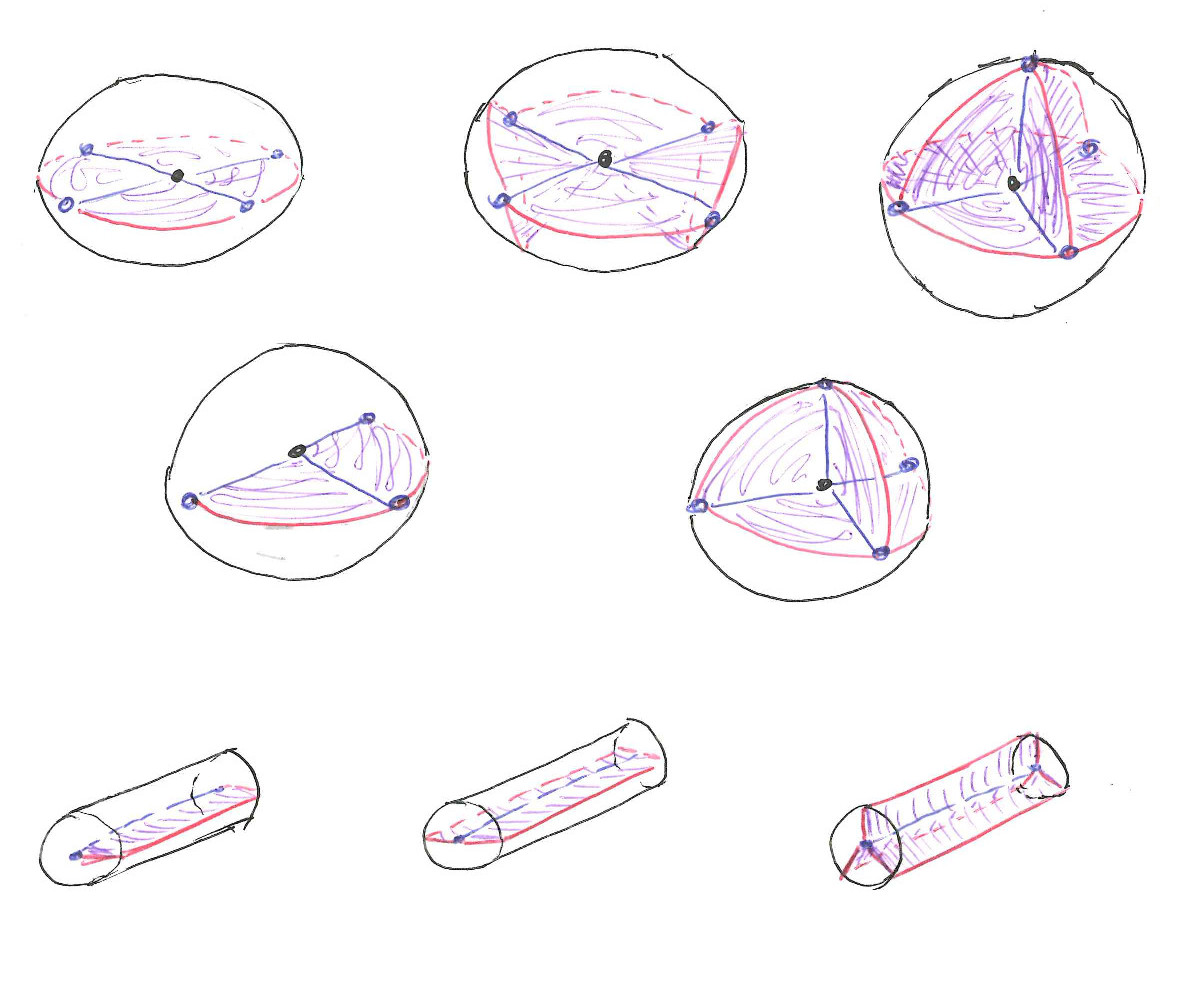
\includegraphics[width=6in]{figures/3thickeningblocks.jpg}
		\label{fig:3thickeningblocks}
	\end{figure}
	
	Building $H_3(U_S(T))$ by adding an appropriate vertex block to $H_3(U_S(T))$ for each vertex of $T$, then connect them together with edge blocks in the unique way that is forced by the combinatorics of $S$ for each edge of $T$.
	Take the product of this space with $\II$.
	The result is a $\II$--bundle over $H_3(U_S(T))$ and generically a $\II^2$--bundle over $U_S(T)$.
	To extend this to $G$, we add 1--handles for each edge in $G$ that is not in $T$.
	Every such edge has at least one 2-handle in $S$ attached over it, and every 2--cell of $S$ attaches over at least one edge added in this step.
	We use the product of our edge blocks with $\II$ as the 4--disc structure for our 1--handles.
	The combinatorics of $S$ and the requirement that $H_4(U_S(G))$ is orientable make these handle attachments unique.
	Our 4--thickening $H_4(U_S(G))$ is once again a $\II$--bundle over $H_3(U_S(G))$ and generically a $\II^2$--bundle over $U_S(G)$.
	The boundary circles of $U_S(G)$, corresponding to 2--cells of $S$ and thus 2--handles of $W$, are now thickened to solid tori in $H_4(U_S(G))$.
	The last step to this construction is the attachment of 2--handles over these solid tori. 
	
	Let $v^*$ be a boundary circle of $U_S(G)$ corresponding to a 2--cell $c_v$ of $S$ with thickening $V^*$ in the boundary of $H_4(U_S(G))$.
	The first thing we must do is specify a canonical 0--framing on $V^*$, which we do by investigating the diagonal of the square fibers $\II$.
	As a subspace of $V^*$, the union of the fibers have the structure of an annulus or a M\"obius strip.
	To see which we get, we turn to the completion of $H_4(U_S(T))$ into $H_4(U_S(G))$ accomplished by attaching 4--dimensional 1--handles.
	At least one such 1--handle corresponded to an edge of $\pd c_v$, and $n$ of them were attached with an orientation reversal in both $\II$ factors.
	If $n$ is even then the diagonal is an annulus and we put the canonical 0--framing as the trivialization that takes one boundary component of that annulus to $S^1\times\{1\}$.
	If $n$ is odd then the diagonal is a M\"obius strip.
	In this case we take a curve that follows one half of the boundary component of the M\"obius strip (i.e. once around $V^*$ in the longitudinal direction along the boundary), then connects to itself via one half positive twist in the orientation of $V^*$ (which is canonically oriented by the canonical orientations of the double intervals $\II$).
	
	With a 0--framing specified, we just need framing coefficients.
	To recover those, we ask how our canonical framing sits inside of $M$.
	This question is well defined because the solid tori we are attaching 2--handles over are the $V^*$ we examined in the proof of Theorem \ref{thm:3bound4}, and the boundaries of these tori are contained in $M$.
	
	The complex $S$ embeds flatly into $W$, and the restriction of that embedding to the 0-- and 1--handles of $W$ is exactly how $U_S(G)$ embeds in $H_4(U_S(G))$.
	Specifically, the zero section of the torus $V^*$ above is the belt sphere of the 2--handle in $W$ corresponding to the 2--cell $c_v$ in $S$.
	This belt sphere is then the attaching sphere of the dual 2--handle in the handle decomposition of $W^*$ and the framing coefficient is then the number of meridinal twists from the 0--framing to the longitude in $V^*$ that is a meridian of $V$.
	Attaching a 2--handles over every such $V^*$'s yields a handle decomposition of a 4--manifold $W^*$ that is dual to the decomposition of $W$ acquired in Theorem \ref{thm:3bound4}.
	We conclude that $W^*$ is the desired cobordism of $(M,\emptyset)$.
\end{proof}

There are a couple of points left to address in this chapter.
The first is that of explicitly recovering the 0--framing curve used in the attachment of 2--handles in Theorem \ref{thm:3stein4}, a necessity for turning this process into an algorithm.
The second is an acknowledgment of the origin of the ideas in this Section.

The 0--framing $L$ is a curve in the shared boundary of $V$ and $V^*$ that is a number of meridinal twists of $V^*$ away a meridian of $V$.
This number is the framing coefficient we equip to the 2--cell of $S$ representing 2--handle attachment over $V^*$ in the construction of $W^*$.

Because $L$ is a longitude of $V^*$, it wraps exactly once around the meridinal direction of $V$, and can thus be realized as a section over $\pd \D$ where $f(V)=\D$.
Let $\D_0$ be the zero section of $V$ as a disc bundle over an interior regular fiber of $V$.
Then the oriented intersection number of $J$ with $D$ yields the framing coefficient.
We compute the framing coefficient for a 2--cell of $S$ in Section \ref{sub:gleams} using this method.


This work is based on that of Costantino and Thurston in \cite{CostThur08} and of Turaev in \cite{Turaev91}.
Theorem \ref{thm:3stein4} in particular is a version of the Turaev Reconstruction Theorem.
Three distinct versions can be found as Theorem 4.1 of \cite{Cost05}, 3.8 of \cite{CostThur08}, and 19.1 of \cite{Turaev91}.
The proof presented is closest in form to that found in \cite{Cost05}.
These selections offer a decent introduction to the theory of shadows of 4--manifolds.
A shadow is a 2--complex with extra structure, and the Stein complex found in this section is almost a shadow.

%\section{Shadows of 3-- and 4--Manifolds}
%\label{sec:shadow}

The building instructions mentioned in the previous section were studied by Turaev in ~\cite{Turaev91} and are called \emph{shadows}.
Shadows are piecewise--linear 2--dimensional structures that live inside of piecewise--linear, compact, oriented 4--manifolds.
The central algorithm of this work uses shadows of 3-- and 4-- manifolds to construct a triangulation of a 4--manifold with a given 3--manifold boundary.

\begin{defn}
  Let $P$ to be a compact topological space.
  If every point $p$ of $P$ has a neighbourhood homeomorphic to an open set in one of the following local models
  \begin{enumerate}
    \item the closed 2--disc $D^2$,
    \item the product of the interval $I=[0,1]$ with the $Y$--shaped graph $K_{1,3}$, or
    \item the cone on the complete graph $K_4$,
  \end{enumerate}
  then $P$ is a \emph{simple polyhedron}.
  \{ FIGURE HERE DEPICTING THE LOCAL MODELS\}
  The set of points which do not have a neighbourhood homeomorphic to an open set in $D^2$ form a 4--valent graph which we call the \emph{singular set} of $P$ and denote by $\Sing (P)$.
  The vertices and edges of $\Sing (P)$ are called the vertices and edges of $P$.
  We call the connected components of $P\setminus\Sing (P)$ the \emph{regions} of $P$.
  
  The local models each have boundary.
  Being a surface, the 2--disc has a well defined boundary.
  In the local model $K_{1,3}\times I$, the boundary consists of the set $(K_{1,3}\times \{0\})\cup (K_{1,3}\times \{1\})\cup (V(K_{1,3})\times I)$, where $V(K_{1,3})$ denotes the vertex set of the graph $K_{1,3}$.
  The boundary points of the cone on $K_4$, defined at $K_4\times I /\sim$, where $\sim$ is defined to be $(x,1)\sim (y,1)$ for any $x,y$, are the points in $K_4\times \{0\}$.
  
  If a point $p$ of $P$ has a neighbourhood homeomorphic to an open set containing a point in the boundary of one of our three local models, then $p$ is a \emph{boundary point} of $P$.
  The set of all boundary points of $P$ is the boundary of $P$ and is denoted by $\pd P$.
  A region of $P$ is \emph{internal} if its closure is disjoint from $\pd P$.
  If $\pd P$ is empty then $P$ is \emph{closed}.
\end{defn}

Simple polyhedra are almost shadows.
To define a shadow, we need to consider simple polyhedra embedded in a 4--manifold.
First, we introduce a concept from simple--homotopy theory.

\begin{defn}
  Let $K$ be a simplicial complex, and let $\tau$, $\sigma$ be simplices so that $\dim \sigma$ is maximal, $\dim\tau=\dim \sigma -1$, and no simplex of dimension $\dim \sigma$ other than $\sigma$ contains $\tau$.
  We obtain the complex $L$ from $K$ by removing $\sigma$ and $\tau$.
  That is, $L= K\setminus(\inter{\sigma}\cup\tau)$.
  We say that $L$ is an \emph{elementary collapse} of $K$.
  
  If a complex $L$ is obtained from $K$ through iterated elementary collapses, then we say that $L$ is a \emph{simplicial collapse} of $K$.
  We may also say that $K$ {\em collapses} onto $L$.   
\end{defn}

We are finally ready to define a shadow.

\begin{defn}
  Let $W$ be a piecewise--linear, compact, oriented 4--manifold.
  Let $P\subset W$ be a closed simple sub--polyhedron of $W$ such that $W$ collapses onto $P$ and the regions of $P$ are \emph{locally flat} in $W$.
  That is to say, if $p$ is in $P\setminus\Sing(P)$ then there is a chart $(U,f)$ of $W$ around $p$ so that $f(P\cap U)$ is contained in $\R^2\subset \R^4$.
  We define $P$ to be a \emph{shadow polyhedron} of $W$.
\end{defn}

\begin{rmk}
  There is a notion of shadow equivalence in~\cite{Turaev91} via basic shadow moves.
  A shadow polyhedron whose regions are all homeomorphic to discs is called \emph{standard}, and through Turaev's shadow moves any shadow polyhedra can be made standard.
  Furthermore, the algorithms which make up the bulk of this document produce a standard shadow polyhedron, so from here forward we always consider our polyhedra to be standard.  
\end{rmk}

Not every piecewise--linear, compact, oriented 4--manifold contains a shadow polyhedron.
A necessary and sufficient condition for the existence of a shadow polyhedron in such a 4--manifold is the existence of a handle decomposition of $W$ containing no handles of index greater than 2, as shown in~\cite{Turaev91}.
This requirement tells us that $W$ has a connected non-empty 3--manifold boundary $M$.
A shadow is defined for $M$ as well.

\begin{defn}
  A shadow polyhedron of an oriented, closed 3--manifold $M$ is a shadow polyhedron $P$ of a compact 4--manifold $W$ with $\pd W=M$
\end{defn}

This gives us the following theorem for free.

\begin{theorem}
  \label{the:shadowexistence}
  Every closed, oriented 3--manifold has a shadow polyhedron.
\end{theorem}

\begin{proof}
  To sketch the proof, we use the results of Lickorish and Kirby as summarized in~\cite{GompStip}.
  Any closed, oriented smooth 3--manifold $M$ has a presentation as integral surgery over a link $L$ in $\sthr$.
  A handle decomposition of a 4--manifold with boundary equal to $M$ can be obtained from the integral surgery diagram of $M$.
  We begin with a 0--handle, which is just a copy of $B^4$ with boundary $S^3$.
  We put our surgery presentation in this $S^3$.
  Each component of the surgery link in $S^3$ will be the attaching sphere of a 2--handle, and the integer surgery coeffifient will be the element of $\pi_1(\gl{2}{\R})$ that fully describes the framing of this 2--handle.
  Adding a 2--handle over every component of the link results in a 4--manifold $W$ such that $\pd W=M$.
 
  The link diagram also determines the shadow of $W$ hence of $M$.
  Take $\pi:L\to \DD$ to be a regular projection.
  That is, $\pi$ is injective everywhere except for at a finite number of points which coincide with the crossings of $L$.
  Then the mapping cylinder $(I\times L)\coprod \DD/(0,x)\sim\pi(x)$ with a disc glued to the free link ends at $\{1\}\times L_i$ is, as per our definition, a shadow of $W$.
\end{proof}

It is natural to wonder how closely related shadows are with their associated 3-- and 4--manifolds.
Just as simple--homotopy type is not a complete invariant of 4--manifolds, a shadow polyhedron does not uniquely determine a 4--manifold.
The following example demonstrates this explicitly and hints at what kind of additional information is needed to uniquely identify a shadow with a 4--manifold.

\begin{ex}
  \label{ex:polypoly}
  We examine disc bundles over $\stwo$.
  Take $W_0$ to be the trivial disc bundle $\D^2\times S^2$ and $W_1$ to be the bundle whose 0--section has self--intersection number of 1 in the ambient 4--manifold.
  Each $W_i$ collapses onto $\stwo$, so each have shadow $\stwo$.
  Because $W_0$ is $\D^2\times S^2$, it's boundary is $S^1\times S^2$.
  One can see that $W_1$ has handle decomposition with exactly one 0--handle $B^4$ and one 2--handle attached over the unknot in $S^3=\pd B^4$ with framing coefficient 1.
  This manifold is a punctured $\CP^2$, so has boundary $S^3$.
  We've defined a shadow polyhedron of an oriented, closed 3--manifold $M$ to be a shadow polyhedron $P$ of a compact 4--manifold $W$ with $\pd W=M$, so $S^3$ and $S^2\times S^1$ each have shadow polyhedron $S^2$.
\end{ex}

We've found a pair of distinct 4--manifolds with distinct boundaries, but the shadow of each is $S^2$.
We want to construct a 4--manifold whose boundary is a given 3--manifold, and this shows that we need more than just a naked shadow polyhedron to do so.
The information needed is carried by the internal regions of a polyhedron and are named ``gleams'' by Turaev.
One can intuit from the Example~\ref{ex:polypoly} that a ``gleam'' might describe the regular neighbourhood of an embedded shadow.

\begin{defn}
  Let $P$ be a polyhedron embedded in the 4--manifold $W$ in a locally flat way.
  Then there exists a canonical colouring of the internal regions of $P$ by elements of $\frac{1}{2}\Z$ called \emph{gleams}.
  A gleam necessarily depends on the embedding of $P$.
  We may also discern a canonical colouring of the internal regions of $P$ by elements of $\Z_2$ called the $Z_2$--\emph{gleam} that depends only on the combinatorial structure of $P$.
  The $Z_2$--gleam of a region of $P$ determines whether the gleam of that region is an integer or half--integer.

  Let $D$ be an internal region of $P$.
  Because $P$ is assumed to be standard, we know that $D$ is an open disc and the closure of $D$ is a closed disc.
  The embedding of $D$ in $P$ extends to an embedding $e : \bar{D} \to P$ so that $e$ takes $\pd\bar{D}$ into $\Sing(P)$.
  Denote by $U(D)$ the simple polyhedron that is a small open regular neighborhood of $D$ in $P$.
  We may construct $U(D)$ from $\bar{D}$ by first gluing the core of either an annulus or M\"obius strip, to $\pd\bar{D}$.
  Then, for each point $p$ of $\pd\bar{D}$ so that $e(p)$ is a vertex of $P$, let $A_p$ be an arc in the band attached to $\pd\bar{D}$ so that $A_p$ intersects the core of the band only at $p$.
  Obtain $U(D)$ by gluing half the boundary of a disc to $A_p$ for each $p$.
  The map $e$ extends easily to the map $e':U(D)\to P$.
  Define the $\Z_2$--gleam of $D$ in $P$ to be equal to $1$ if the band attached to $\pd\bar{D}$ was a M\"obius strip and $0$ if the band was an annulus.
  
  \{FIGURE: $U(D)$ FOR $Z_2$--GLEAM EVEN AND ODD\}
  
  Now, suppose that $f:P\to W$ is our locally flat embedding of $P$ and let $D, \bar{D}, e: D \to P, U(D)$ and $e'$ be defined as before.
  Because $e'$ embeds $U(D)$ in $P$, we consider $U(D)$ to be a subset of $P$.
  A regular neighbourhood of $f(U(D))$ in $W$ collapsing onto $f(U(D))$ is an oriented 4--ball $B^4$.
  Let $p_0$ be a point in $\pd\bar{D}$ and $(V,g)$ a chart of $W$ with $V$ containing $p_0$ such that the intersection $V_P = V\cap f(U(D))$ is contained in $f(U(D))$.  
  The embedding $f$ is locally flat, so $g(V_P)$ is contained in a 3--dimensional slice $B^3$ of $g(V)$ and $g(f(\bar{D})\cap V)$ is contained in a 2--dimensional slice of $B^3$.
  If $p_0$ is not a vertex of $P$, then there are exactly two other regions $D'$ and $D''$ of $P$ that meet $D$ at $p_0$.
  The direction in $B^3$ in which $D'$ and $D''$ separate away from $p_0$ can be extended to a direction in $g(V)$ where it is an element of the projective line $P^1$ of lines orthogonal to $f(D)$ sufficiently close to $f(p_0)$.
  If $p_0$ is a vertex of $P$, then ignoring the region of $P$ that meets $D$ only at $p_0$ leaves two suitable separating regions that meet $D$ at $p_0$.
  We form a smooth bundle of directions over $\pd\bar{D}$ which is a section of a $P^1$ bundle over $\pd\bar{D}$.
  The obstruction to extend this section to all of $D$ is a class of $H^2 (D, \pd D; \pi_1 (P^1 ))$.
  The ambient space $g(V)$ is oriented so $D$ is oriented.
  The class of $H^2 (D, \pd D; \pi_1 (P^1 ))=\Z$ is an integer $z$ that corresponds to the number of times a section of the boundary of $D$ loops around a $P^1$ bundle, which is the number of half loops made around a $S^1$ bundle.
  We are interested in the $S^1$ bundle, so we take the gleam of $D$ to be $z/2$.
  Note that $z$ modulo 2 is exactly the $\Z_2$--gleam of $D$.
\end{defn}

\begin{theorem}\cite{Turaev91}
  \label{the:turaevreconstruction}
    Let $S$ be a polyhedron whose internal regions are equipped with gleams.
    Then there exists a canonical construction associating to $S$ the a pair $(W,S)$, where $W$ is a piecewise--linear, compact, oriented 4--manifold $W$ containing an embedded copy of $S$ with shadow $S$ can be reconstructed from the combinatorics of $S$.
\end{theorem}

We can extend our definition of shadows to shadows of pairs $(M,G)$ where $M$ is a 3--manifold whose boundary is not necessarily empty and $G$ is an embedded framed graph whose vertices have degree either 1 or 3.
This extension is useful because it allows us to build a shadow for a closed 3--manifold from a reasonable decomposition into blocks whose shadows are known.
In this case, the polyhedron representing our shadow will have boundary and the 1--cells of the boundary will be classified.

\begin{defn}
  Define a \emph{boundary--decorated} standard polyhedron to be a standard polyhedron $P$ with boundary so that $\pd P$ is a graph whose edges are coloured one of $i$ for internal, $e$ for external, or $f$ for false.
  The graph $\pd P$ then has three distinct subgraphs $\pd_i P$, $\pd_e P$ and $\pd_f P$ intersecting only at vertices and whose union is $\pd P$.
  If $\pd_f P=\emptyset$ then we call $P$ as \emph{proper}.
\end{defn}

Boundary decorated polyhedra can be turned into a shadows for a 3--manifolds with boundary and with framed graphs embedded in their interior.
The boundary of the 3--manifold is represented by the subgraph $\pd_e P$ and the embedded graph is represented by the subgraph $\pd_i$.

\begin{defn}
  Let $P$ be a boundary decorated standard polyhedron properly embedded in a 4--manifold $W$ so that $W$ collapses onto $P$ with a framing on $\pd_i P$.
  An embedding $f:X\to Y$ is \emph{proper} if $f(\pd X) = f(X)\cap \pd Y$ and $f(X)$ is transverse to $\pd Y$ everywhere in $\pd X$.
  
  Let $M$ be the complement of an open regular neighbourhood of $\pd_e P$ in $\pd W$ and let $G$ be a framed graph embedded in $M$ whose core is $\pd_i P$.
  Then $P$ is a \emph{shadow} of the pair $(M,G)$.
  If the false boundary is empty, then $P$ is a \emph{proper} shadow of $(M,G)$.
  Gleams are defined on the interior regions of $P$ as before.
\end{defn}





\chapter{Algorithms}
\label{cha:algorithm}
\label{cha:alg1}

This final chapter develops and details a composite of algorithms that takes as input an edge--distinct triangulation $T$ of a 3--manifold $M$, and produces a triangulation of a 4--manifold $W$ whose boundary is $M$.
Section \ref{sec:3bound4} outlines the general flow we follow.

We begin with a triangulation $T$ of a 3--manifold $M$.
First we find suitable map from $T$ to the 2--disc.
This map yields a Stein complex.
The Stein complex provides instructions for building a triangulation for 4--manifold $W$ whose boundary is $M$.

\section{The Generic Piecewise--linear Map}
\label{sec:proj}
The data we are trying to collect and retain with the algorithms of this chapter are as follows:
\begin{enumerate}
  \item A list of polygons which we will call regions.
  \item A colouring of every edge of every region using one of the three colours $i,f,h$.
  \item A wedge number of $0$, $1$, or $2$ for any edge coloured $i$.
  \item A list of adjacencies between regions.
        An item in this list consists of a pair of regions and an $i$--coloured boundary edge of each region.
  \item A list of piecewise--linear circles associated to each region.
        An item in this list is an ordered list of polygonal 2--cells which live in a closed polyhedral 3--complex so that any two consecutive 2--cells lie on the boundary of the same 3--cell, yet any 3--cell contributes either zero or two 2--cells to any given list.  This list is indexed by the list of regions in item 1.
\end{enumerate}
This data is sufficient to build a shadow, as seen in Chapter \ref{cha:shadow}.


	\subsection{Piecewise--linear Maps and 2--complexes}
	\label{sub:2complex}
	We establish some properties of piecewise--linear maps from polyhedra to $\C$, and develop an algorithm to produce an associated 2--dimensional CW--complex.
This CW--complex is used as a data type to keep track of the piecewise linear version of the generic proper smooth maps of Section \ref{sec:3bound4}.
In Section \ref{sec:stein}, we use the 2--complex produced to form a Stein complex.

\begin{defn}
	\label{def:stdproj}
	Let $\sigma$ be a tetrahedron with the four vertices $u$, $v$, $w$, $x$, six edges $uv$, $uw$, $ux$, $vw$, $vx$, $wx$, and faces $\hat{u}$, $\hat{v}$, $\hat{w}$, $\hat{x}$, where a face is named by the vertex of $\sigma$ it does not contain.
	Define a projection $\pi: \sigma\to\C$ by first choosing a map from the vertices of $\sigma$ to distinct points in $\sone$.
	Each point $p$ of $\sigma$ is described by the convex combination
	\[
		p = t_u u + t_v v + t_w w + t_x x
	\]
	with the $t_*$ nonnegative and summing to 1.
	We can define $\pi$ at $p$ by
	\begin{eqnarray}
		\label{affine_extension}
		\pi(p)
		&=&
		\pi(t_u u + t_v v + t_w w + t_x x) \nonumber \\
		&=&
		t_u \pi(u) + t_v \pi(v) + t_w \pi(w) + t_x \pi(x)
	\end{eqnarray}
	  
	Without loss of generality, we assume that the points $\pi(u),\pi(v),\pi(w),\pi(x)$ are ordered in a clockwise orientation about $\sone$.
	We call $\pi:\sigma\to\C$ a \emph{linear tetrahedral projection}.
\end{defn}

\begin{defn}
	\label{def:projpttypes}
	A point of $\C$ in the image of $\pi$ is one of five types:
	\begin{enumerate}
		\item The four points of type 1 are the images of the vertices of $\sigma$ under $\pi$.
		\item The single point of type 2 is the intersection $\pi(uw)\cap\pi(vx)$.
		\item All points in $\pi(uv)\cup\pi(vw)\cup\pi(wx)\cup\pi(xu)$, excluding the points of type 1, are of type 3.
		\item All points in $\pi(uw)\cup\pi(vx)$ excluding the points of type 1 or 2 are of type 4.
		\item The points of type 5 are the points outside of the image of any vertex or edge of $\sigma$.
	\end{enumerate}
\end{defn}

By definition, the preimage of a point of type 1 is a vertex of $\sigma$.
The preimage of the single point of type 2 is a line segment between the edges $uw$ and $vx$ interior to $\sigma$.
A point of type 3 is the image of exactly one point in an edge of $\sigma$.
A point of type 4 is in the image of exactly one edge and one face, so the preimage of one of these points is a line segment interior to $\sigma$ between those two facets.
Finally, points of type 5 are in the image of exactly two faces of $\sigma$, and pull back to line segments interior to $\sigma$ between those two faces.
Our classification of points in the image of $\pi$ naturally lends itself to the structure of a 2--complex.
We detail this construction in Algorithm \ref{alg:lintet2complex}.

\begin{algorithm}
	\caption{Generating a 2--complex from a linear tetrahedral projection}
	\label{alg:lintet2complex}
	\KwData{a simplex $\sigma$, a map $\pi:\sigma\to\C$}
	\KwResult{a 2--complex $X$}
	\Begin{
		$X^1 \longleftarrow \sigma^1$\;
		\While{there is a pair of edges $(e,f)=((u,v),(w,x))$ in $X$ that cross at the point $y\in\RR$}{
			delete $e$, $f$\;
			add a vertex $y'$ to $X$\;
			define $\pi(y')=y$\;			
		}
		\ForEach{chordless cycle $c=(v_1,v_2,\dots,v_k,v_1)$ in $X$}{
			attach a 2--cell over $c$\;
		}
	}
\end{algorithm}

For $T$ a 3--dimensional edge--distinct connected simplicial complex, the above algorithm breaks down when a triple of edges cross at the same point.
A sufficient condition to guarantee that a crossing point between a pair of edges is the crossing point of at most two edges (by the results in \cite{PoonRub98}) is if $\pi(T^1)$ is a subgraph of an odd dimensional complete graph $K_n$ in its standard position (i.e.\ with the $n$ vertices each at a distinct $n\nth$ complex root.)

\begin{defn}
	Let $T$ be a 3--dimensional edge--distinct connected simplicial complex and $\pi:T\to\C$ a map that is linear on each simplex of $T$.
	If, for some odd positive integer $n$, $\pi(T^0)$ is injective into the $n\nth$ roots of unity, then we say $\pi$ is a \emph{crossing distinct} projection of $T^1$ into $\C$.
\end{defn}

The 2--complex construction can now be extended to simplicial complexes.
In Algorithm \ref{alg:crossdis2complex} we continue to let $T$ be a 3--dimensional edge--distinct connected simplicial complex with crossing distinct projection $\pi:T\to\C$.

\begin{algorithm}
	\caption{Generating a 2--complex from a crossing distinct projection}
	\label{alg:crossdis2complex}
	\KwData{ $T$, $\pi:T\to\C$}
	\KwResult{a 2--complex $X$}
	\Begin{
		$X^1 \longleftarrow T^1$\;
		\While{there is a pair of edges $(e,f)=((u,v),(w,x))$ in $X$ that cross at the point $y\in\RR$}{
			delete $e$, $f$\;
			add a vertex $y'$ to $X$\;
			define $\pi(y')=y$\;			
		}
		\ForEach{chordless cycle $c=(v_1,v_2,\dots,v_k,v_1)$ in $X$}{
			attach a 2--cell over $c$\;
		}
	}
\end{algorithm}
	
	\subsection{Tetrahedral Truncation}
	\label{sub:truncttet}
	We are interested in what happens to the 2--complex obtained in Section \ref{sub:2complex} when we begin truncating tetrahedra.
Truncation must be done in a controlled way, to keep gluing maps between faces well--defined.
A model truncated tetrahedron can be seen in Figure \ref{fig:truncttet}

\begin{figure}
	\centering
	\captionsetup{justification=centering}
	\caption{A truncated tetrahedron}
	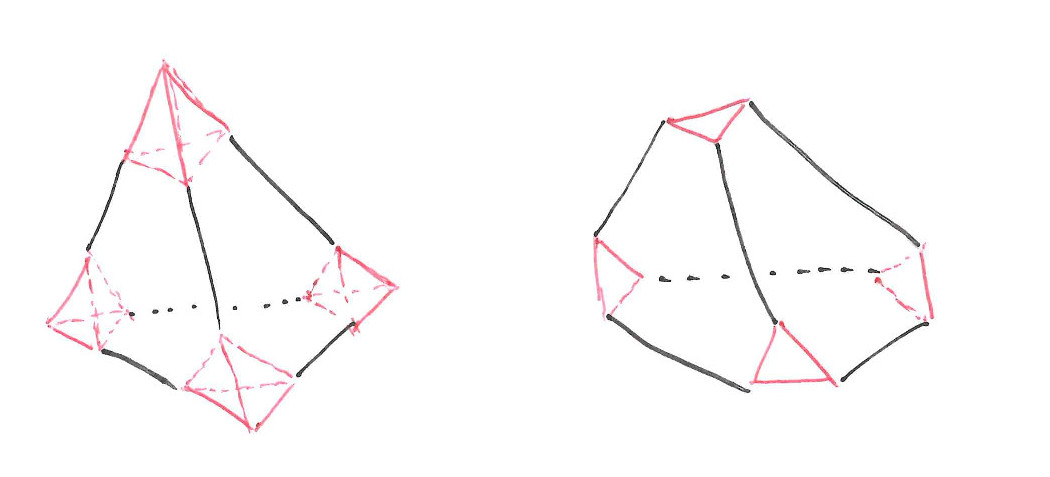
\includegraphics[height=2in]{figures/truncttet.jpg}
	\label{fig:truncttet}
\end{figure}

Let $T$ be a 3--dimensional edge--distinct connected simplicial complex and $\pi:T\to\C$ a crossing distinct projection of $T^1$ into $\C$.
One way to turn each tetrahedron of $T$ into a truncated tetrahedron is to remove a neighbourhood from each vertex of $T$.
Each ball removed leaves a $\DD$ boundary in each truncated tetrahedron that contained the removed vertex.
Once all removals are complete, we have a polyhedral gluing complex whose polyhedral 3--cells are truncated tetrahedra.
We choose the removed balls so that if $B$ is the ball removed about the vertex $v$ in $T^0$, then $B = \pi\inv(B_\varepsilon(\pi(v)))$ where $B_\varepsilon$ is a ball of radius $\varepsilon$ about $\pi(v)$.
Figure \ref{fig:neuter} depicts this process.

\begin{figure}
	\centering
	\captionsetup{justification=centering}
	\caption{Balls to remove and the effect of Algorithm \ref{alg:neuter} on the 2--complex}
	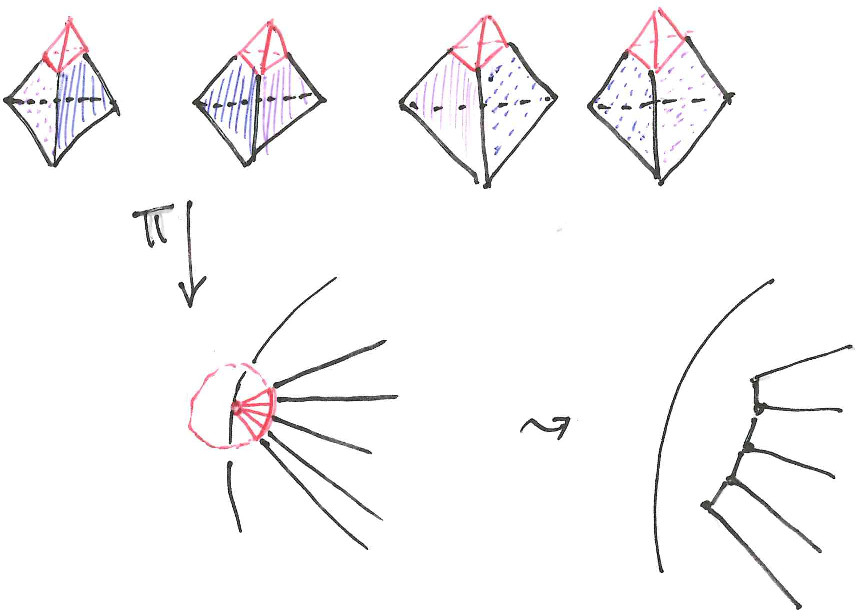
\includegraphics[height=4in]{figures/neuter.jpg}
	\label{fig:neuter}
\end{figure}

We also make explicit the effect this has on the 2--complex we recover from $\pi':T'\to\C$, where $\pi'$ is just $\pi$ restricted to $T'\subset T$.
This is done in Algorithm \ref{alg:neuter}, taking $T$ and $\pi$ to be as in the input to Algorithm \ref{alg:crossdis2complex}.
Figure \ref{fig:neuter} depicts the result of an application around a specific vertex.

\begin{algorithm}[h]
	\caption{Generating a 2--complex from a truncated linear tetrahedral projection}
	\label{alg:neuter}
	\KwData{$T$, $\pi:T\to\C$}
	\KwResult{a 2--complex $X'$ corresponding to the truncated complex $T'$}
	\Begin{
		$X \longleftarrow$ result of Algorithm \ref{alg:crossdis2complex} applied to $T$ \;
		\ForEach{vertex $v$ of $X$ with $v\in\pi(T^0)$}{
			delete all 2--cells containing $v$\;
			\ForEach{edge $e=(v,u)$ of $X$}{
				\ForEach{edge $f=(v,w)$, $f\neq e$}{
					temporarily label $w$ by $\theta_{u,w}$, the positive clockwise rotation in radians about $v$ that takes $e$ onto $f$\;
				}
				delete $e$\;
				add a vertex $u_v$ to $X$\;\label{line:vertexadd1}
				add an edge $(u_v,u)$ to $X$\;
			}
			\ForEach{vertex $u_v$ added at Line \ref{line:vertexadd1}}{
				$w_v\longleftarrow$ the vertex with smallest $\theta_{u,w}$ between $0$ and $\pi$\;
				add an edge $(u_v,w_v)$ to $X$\;
			}
			delete $v$\;
		}
	}
\end{algorithm}
	
	\subsection{Edge Blowups}
	\label{sub:edgeblowup}
	We truncate simplicial complexes because we want to be able to perform edge blowups.
Let $T'$ be a truncated simplicial complex as defined in Section \ref{sub:truncttet}, let $E$ be an internal edge of the polyhedral gluing with $\pd E=(u,v)$ where each of $u$, $v$ are boundary vertices of $T'$, and let $\sigma$, $\tau$ be 3--cells of $T'$ with $\sigma\cap\tau=E$.
A blowup of $E$ across $\sigma$ and $\tau$ is the process of replacing $E$, $\sigma$ and $\tau$ by $\hat{E}$, $\hat{\sigma}$ and $\hat{\tau}$ where $\hat{E}$ is a rectangular 2--cell and $\hat{\sigma}$, $\hat{\tau}$ are 3--cells with $\hat{\sigma}\cap\hat{\tau}=\hat{E}$.
This does not modify any of the other adjacencies of $\sigma$ or $\tau$.
A model blowup is depicted in Figure \ref{fig:edgeblowup}.
The explicit modification of $T'$ involves replacing a small cylinder containing $E$ with a small cylinder that contains $\hat{E}$ in its place.
We then need to define $\pi'$ on this cylinder.
There is already definition of $\pi'$ on the boundary of the cylinder, so we define $\pi'$ on the edges of $\hat{E}$ internal to $T'$ to be a pair of lines that are parallel to $\pi'(E)$, and extend linearly.
Note that there are exactly two ways to define $\pi'$ on $\hat{E}$ that correspond to flipping $\pi'(\hat{E})$ over a central axis.

The effect an edge blowup has on the 2--complex associated to $T'$ is depicted in Figure \ref{fig:edgeblowup2complex}.
The level of bookkeeping involved in writing an explicit algorithm only serves to obfuscate understanding so, because Figure \ref{fig:edgeblowup2complex} depicts a representative case of modification, we take the figure to be a full demonstration.

\begin{figure}
	\centering
	\captionsetup{justification=centering}
	\caption{Blowing up an edge in a polyhedral gluing}
	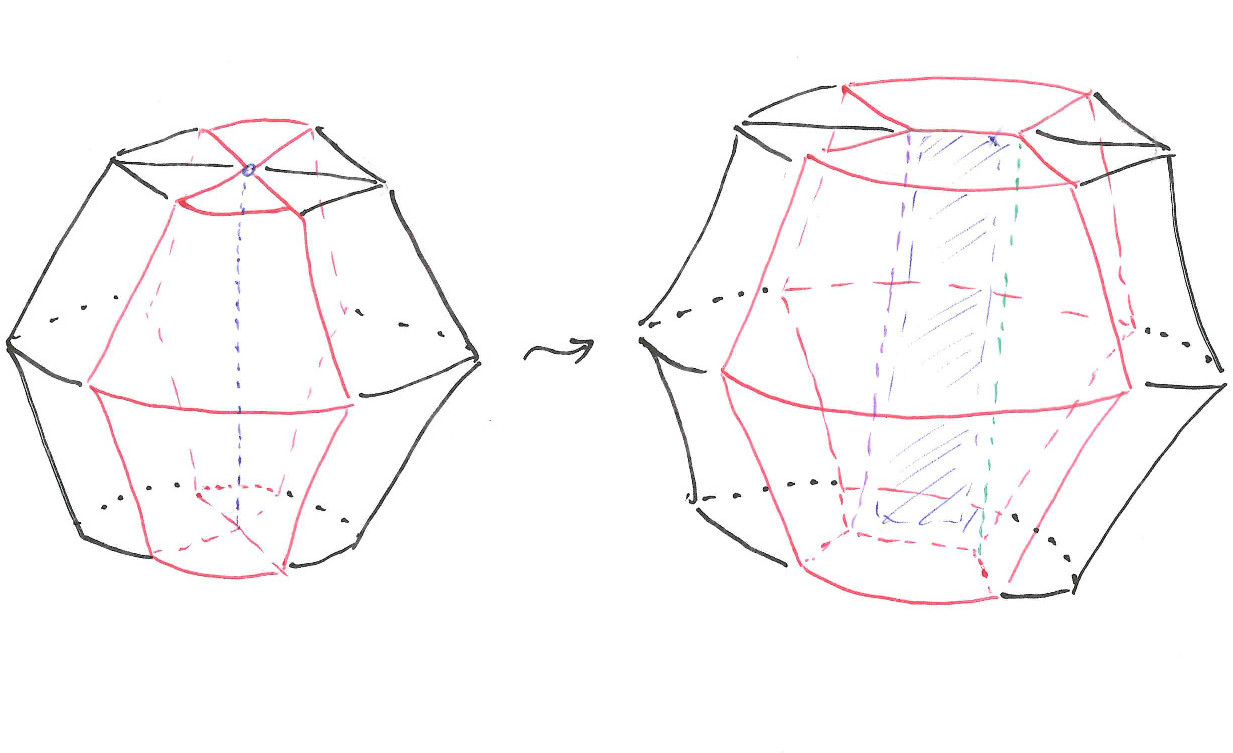
\includegraphics[width=5.5in]{figures/edgeblowup.jpg}
	\label{fig:edgeblowup}
\end{figure}

\begin{figure}
	\centering
	\captionsetup{justification=centering}
	\caption{Blowing up the associated path in the 2--complex}
	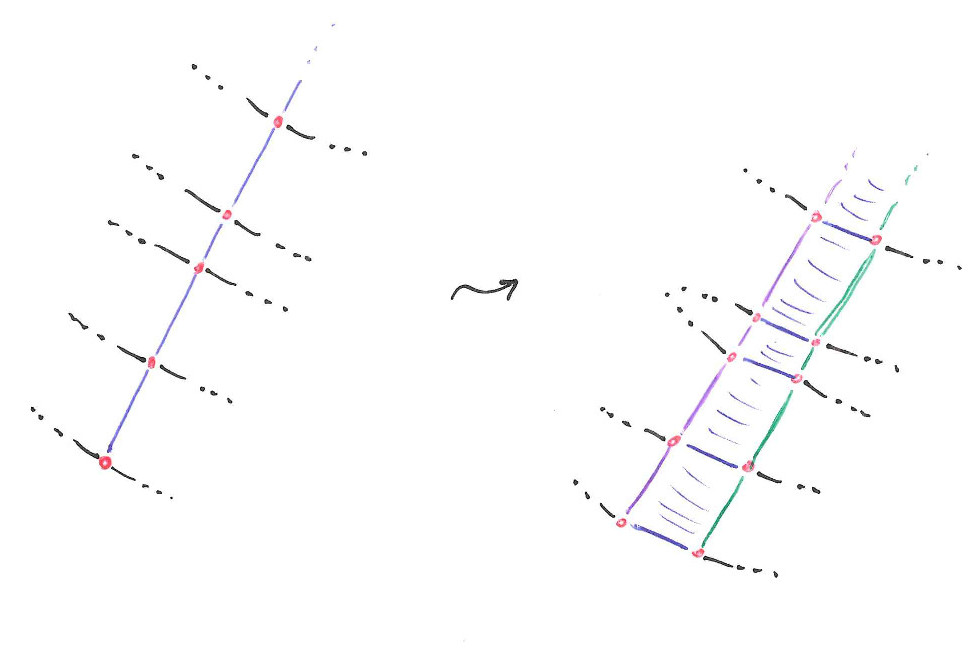
\includegraphics[height=3in]{figures/edgeblowup2complex.jpg}
	\label{fig:edgeblowup2complex}
\end{figure}
	
	\subsection{Triangulations and Dual Complexes}
	\label{sub:tridual}
	An edge distinct triangulation $T$ of a closed, connected, orientable 3--manifold is a simplicial complex that can be run through the algorithms of the previous sections.
We also consider the dual polyhedral complex to $T^*$ and observe how it changes as $T$ is changed.

To begin, let $\pi:T\to\C$ be a crossing distinct projection, and let $X$ be the 2--complex produced by Algorithm \ref{alg:crossdis2complex}.
We want $\pi$ to be the piecewise--linear analogue to the generic, proper, smooth map of Section \ref{sec:3bound4}.
Because $\pi$ is linear on each tetrahedron of $T$, the only analogues to critical values would occur on the images of edges of $T$.
This leaves the 2--cells of $X$ as our analogue to regions of regular values.
Under the classification in from Definition \ref{def:projpttypes}, these are points of type 5.
Restricting our focus to a single tetrahedron $\sigma$, a point of type 5 would pull back through $\pi$ to a line segment $s$ in $\sigma$ that intersects the faces $F^i(\sigma)$ and $F^j(\sigma)$.
Because $p$ is continuous and $T$ is closed, there are tetrahedra $\sigma_i$ and $\sigma_j$ that are incident to $\sigma$ over $F^i(\sigma)$ and $F^j(\sigma)$.
Then $s$ meets the endpoints of two more line segments that pass through $\sigma_i$ and $\sigma_j$.
This continues until the segments join up into a simplicial circle interior to $T$, just as in the smooth regular value theorem.

\begin{algorithm}
	\caption{Building a collection of circles that map over a region}
	\label{alg:regularcircles}
	\KwData{a 2--cell $c$ of $X$, $T$, $T^*$, $\pi:T\to\C$}
	\KwResult{a collection $C=\{C_i\}$ of oriented simplicial circles in $T^*$ representing the circles in $T$ that project through $\pi$ over the region in the plane that correspond to $c$}
	\Begin{
		$c_\pi\longleftarrow$ the region of type 5 points in the plane corresponding to $c$\;
		$C\longleftarrow\emptyset$\;
		\ForEach{edge $o^*$ in $T^*$}{
			\If{the dual 2--cell $o$ in $T$ has $c_\pi\subset\pi(o)$}{
				add $o^*$, including its boundary vertices, to $C$\;
			}			
		}
		orient the edges of $C$ by the orientation of $T$\;
	}	
\end{algorithm}

The circles we find this way unambiguously define cycles in the 1--skeleton of $T^*$, the dual complex to $T$, so we also take the result Algorithm \ref{alg:regularcircles} to be the corresponding dual cycles.
We use the dual complex as a central data structure alongside the 2--complex $X$ to store information about $\pi$.
The first example of this is in Algorithm \ref{alg:regularcircles}, where we find all of the simplicial circles in $T^*$ that map over a region of $X$.
We produce $C$, a collection of disjoint simplicial circles in $T^*$ that project over $c_\pi$, the region of type 5 points in the plane corresponding to $c$, and we decorate the associated 2--cell $c$ of $X$ by a positive integer: the number of connected components of $C$.

In Section \ref{sub:truncttet}, we deleted balls about each vertex of $T$ to find $T'$.
The best we can do to reflect this modification in $T^*$ is to delete the interior of each 3--cell.
This modification yields a 2--complex $T'^*$ and preserves the simplicial circles found during Algorithm \ref{alg:regularcircles}.

In Section \ref{sub:edgeblowup} we blew up edges into 2--cells.
By duality of dimension, the appropriate action to consider would be to split a 2--cell by an edge.
An edge $o^*$ of $T'^*$ connects vertices that are dual to 3--cells.
These 3--cells are adjacent over the 2--cell $o$ that is dual to $o^*$.
We can therefore consider an edge in $T'^*$ to indicate adjacency between a pair of 3--cells.

Let $E$ be the edge and $\sigma$, $\tau$ be the 3--cells that we blow up.
The modification of $T'^*$ appropriate to a blowup over $E$ then begins by introducing a 1--cell $\hat{E}^*$ into $T^*$ over the vertices $\hat{\sigma}^*$ and $\hat{\tau}^*$.
We then remove $E^*$ and introduce a pair of 2--cells corresponding to the new edges of $\hat{E}$ over the newly created chordless cycles containing $\hat{E}^*$.
We can see the modified structure in Figure \ref{fig:dualblowup}.

\begin{figure}
	\centering
	\captionsetup{justification=centering}
	\caption{Dual edge blowup}
	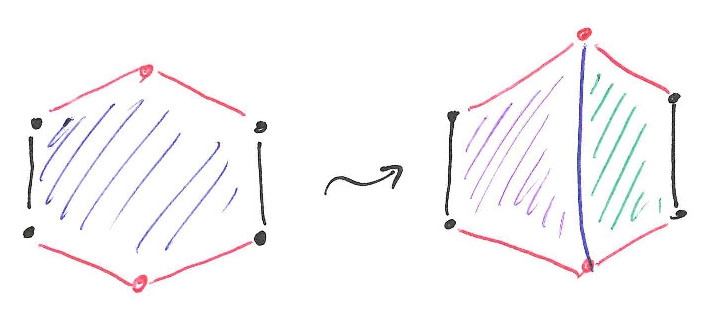
\includegraphics[width=5.5in]{figures/dualblowup.jpg}
	\label{fig:dualblowup}
\end{figure}

It is worth noting here that we need only build directly the collection of circles that map over a single region.
Once that is built, the circles mapping over neighbouring regions are determined from our first collection.
This is especially useful once edges are blown up, as tracking the specifics of a projection $\pi$ through such modifications is tedious.

Let $X$ be a 2--complex generated as described by any of our algorithms from a polyhedral gluing $T$ and let $T^*$ be the appropriate dual complex to $T$.
Let $c$ be a 2--cell of $X$, let $c'$ be a neighbouring 2--cell over the edge $e$ in $X$, let $C$ be the collection of circles mapping over $c$, and $C'$ the collection over $c'$.
There is an edge $E$ of $T$ and dual 2--cell $E^*$ that correspond to $e$.
By Algorithm \ref{alg:regularcircles} the only set of edges in $T^*$ on which $C$ and $C'$ differ is $\pd E^*$.
We can then obtain $C'$ from $C$ by taking the symmetric difference of $C$ with $\pd E^*$, which we denote by $C'=C\triangle \pd E^*$.
	
	\subsection{Genericity Via Blowups}
	\label{sub:genericity}
	In Section \ref{sub:tridual} we mentioned that we would like $\pi$ to be the piecewise linear analogue to the generic proper smooth map of Section \ref{sec:3bound4}.
The important condition that we do not necessarily have is genericity.
An investigation of the analogue to critical points of $\pi$ demonstrates why an appropriate choice of edge blowups will introduce the genericity we are looking for.

Generic singular fibers in the smooth case have the form of either a point or a figure 8 graph.
Taking $T$, $\pi:T\to\C$, and $X$ be as in Section \ref{sub:tridual}.
A singular fiber of a $\pi$ is found by checking how simplicial circles change when we pass over the images of edges in $T$.
Let $X(c_i)$, $X(c_j)$ be 2--cells in $X$ that intersect at a 1--cell $X(e)$, let $c_i$, $c_j$ be the regions of points of type 5 in the plane corresponding to $X(c_i)$, $X(c_j)$, and let $e$ be the strand of points of type 4 that corresponds to $X(e)$.
Let $E$ be the edge of $T$ with $e\subset\pi(E)$, let $C_i=\{C_{i,k}\}$ be the collection of simplicial circles in $T^*$ that correspond to the circles of $T$ that map through $\pi$ over $c_i$, and let $C_j=\{C_{j,l}\}$ be the similar collection for $c_j$.
Considering $C_i$ and $C_j$ as sets of edges in $T^*$, the method of building $C_i$ and $C_j$ found in Algorithm \ref{alg:regularcircles} tells us that the symmetric difference of $C_i$ and $C_j$ is either the boundary of the dual 2--cell $E*$, or is empty.

The form of the singular fiber over a point in $e$ is then seen by pulling the centres of the edges of $\pd E^*$ towards the centre of $E^*$.
This is justified by considering the centre of $E^*$ as the sole intersection of $E$ and $E^*$, and recognizing that the preimage of a point in $e$ through $\pi$ must intersect the edge $E$.
We illustrate this situation in Figure \ref{fig:plsingularities}.

\begin{figure}
	\centering
	\captionsetup{justification=centering}
	\caption{Simplicial circles near an edge}
	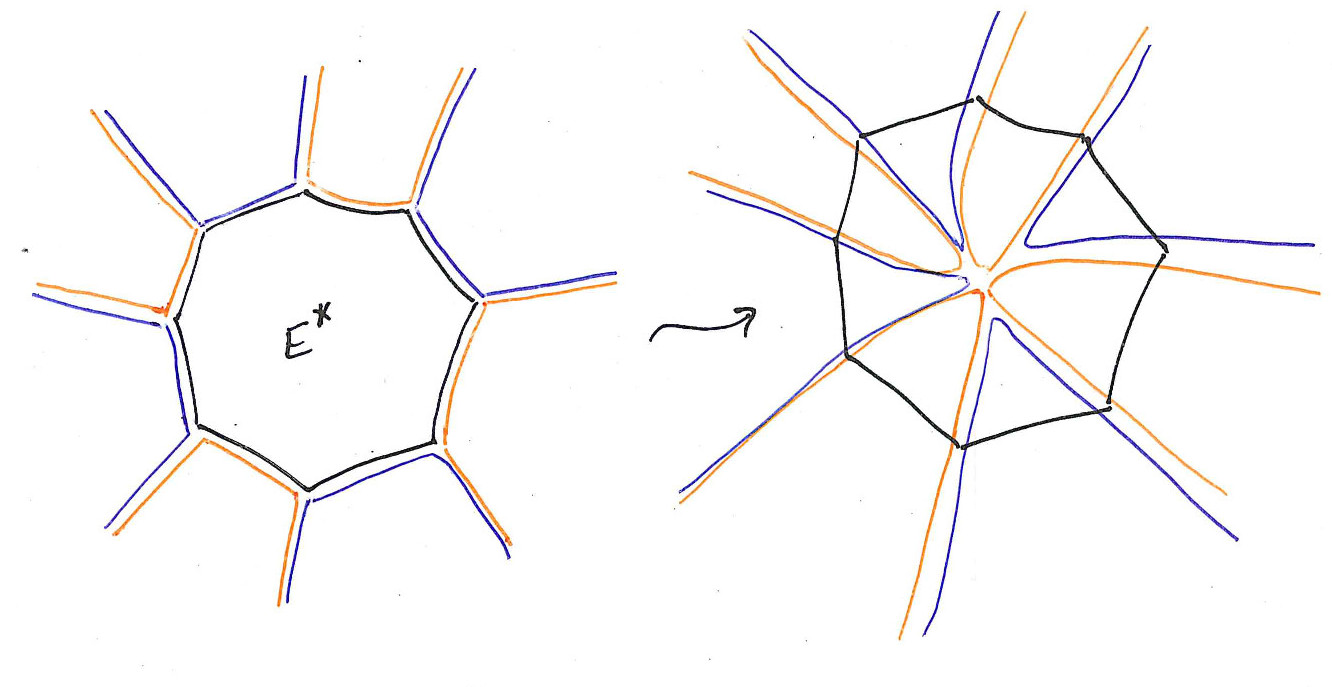
\includegraphics[height=3in]{figures/plsingularities.jpg}
	\label{fig:plsingularities}
\end{figure}

The form of the singular fiber is then the wedge of $n$ simplicial circles.
We define $n$ to be the \emph{wedge number} of $E$, and this can be computed by investigating the link of $E$ in $T$ through $\pi$, which is precisely what we do in Algorithm \ref{alg:computewedgenum}.

\begin{algorithm}[h]
	\caption{Wedge number computations}
	\label{alg:computewedgenum}
	\KwData{$T$, $\pi:T\to\C$, and edge $E$ of $T$}
	\KwResult{the wedge number of $E$, denoted $w_E$}
	\Begin{
		$C\longleftarrow\lk{E}=\{e_0,e_1,\dots,e_k,e_0\}$ as a cycle of the graph $T^1$\;
		$w_E\longleftarrow 0$\;
		\ForEach{edge $e$ in $C$}{
			\If{$\pi(e)$ crosses $\pi(E)$}{
				$w_E\longleftarrow w_E+1/2$\;
			}
		}
	}
\end{algorithm}

Using the fact that $T$ is closed, we get that $\lk{E}$ is a simplicial circle in the 1--skeleton of $T$.
Because $\pi$ maps the vertices of these circles to $S^1\subset\C$, we classify the edges in $\lk{E}$ into those that pass over $e=\pi(E)$ and those that do not.
There is an even number of edges that cross $e$ because $\lk{E}$ is closed.
An edge $F$ of $\lk{E}$ with $f=\pi(F)$ crossing $e$ determines uniquely a tetrahedron $\sigma$ with $F,E\in\sigma^1$.
For $x_i\in c_i$ and $x_j\in c_j$, take $\gamma$ to be a simple path from $x_i$ to $x_j$ that crosses $e$ transversely exactly once.
Then $\pi\inv(x_i)$ and $\pi\inv(x_j)$ each intersect $\sigma$, and the preimage of every point in $\gamma$ does so as well.
A representative of this situation is seen in Figure \ref{fig:gammapullback}.
To turn $\pi\inv(x_i)$ into $\pi\inv(x_j)$ along $\gamma$, the simplicial circle passes through $\sigma$ and over $E$.

\begin{figure}
	\centering
	\captionsetup{justification=centering}
	\caption{Preimages of points on either side of $e$ as they sit in $\sigma$}
	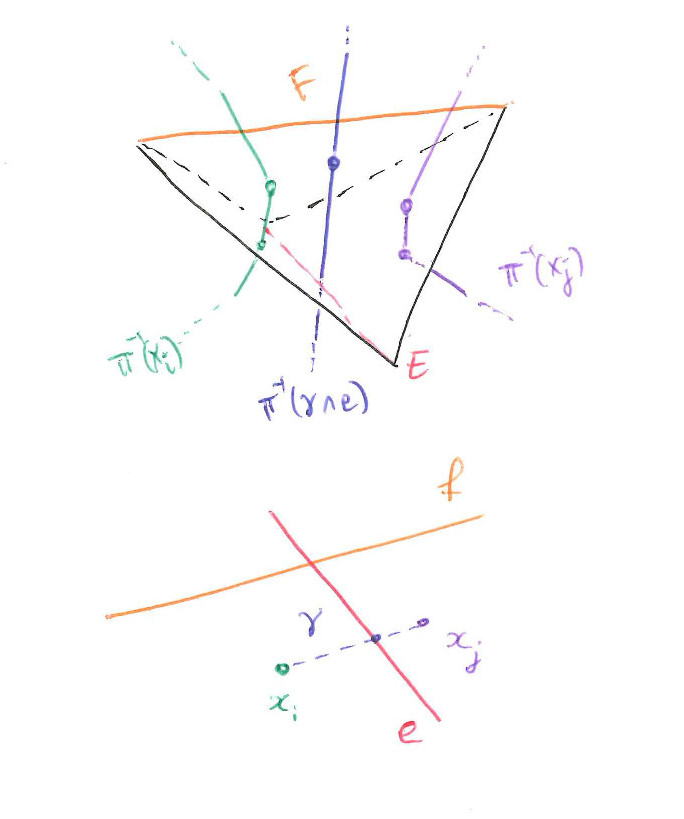
\includegraphics[width=3.75in]{figures/gammapullback.jpg}
	\label{fig:gammapullback}
\end{figure}

The edges of $\lk{E}$ that do not cross $e$ determine tetrahedra that do not have this property.
Each edge of $\lk{E}$ that crosses $e$ then contributes one half of one circle in the bouquet of circles that map over $e$, hence contributes $+1/2$ to the computation of the wedge number.

We strive for the piecewise analogue of genericity and this happens when the wedge number of each edge in $T$ is 0, 1, or 2.
One way to achieve this is through the use of edge blowups.
In order to perform edge blowups, we modify our triangulation to a truncated triangulation.
Truncating in this way and then performing edge blowups makes tracking data through edges more trouble than its worth, and leads to confusion.
Instead, we turn to the dual decomposition for a better way.

We keep $T$ as our 3--manifold triangulation and $T^*$ as its dual.
Let $E$ be an edge of $T$ with dual 2--cell of $E^*$.
The computation of a wedge number for $E$ assigned each edge in $\lk{E}$ a contributing coefficient of $0$ or $+1/2$.
In the justification of this assignment, it was demonstrated that the contribution comes from the tetrahedrons uniquely determined by the edges of $\lk{E}$ rather than the edges themselves.
For each edge $E$ of $T$ (2--cell $E^*$ of $T^*$), the tetrahedra containing $E$ (the vertices in the boundary of $E^*$) are assigned a wedge coefficient of 0 or $+1/2$.
The wedge number for $E$ ($E^*$) is then computed as the sum of the wedge coefficients surrounding it.

Recall that the modification to $T^*$ equivalent to an edge blowup was the splitting of a 2--cell by a new edge.
In the view from $T$, the 3--cells over which we blowup still contain and map over each of the new edges, while the remaining 2--cells contain only one of the edges.
The 3--cells over which we split then contribute to the wedge numbers of both edges, while the rest contribute to only one.

In $T^*$, we have split a 2--cell by a 1--cell connecting a pair of vertices.
The vertices over which we connect contribute their wedge coefficient to both of the new 2--cells because the corresponding 3--cells project over both of the new edges.
The wedge numbers of the new 2--cells are then easily recomputed as displayed in Figure \ref{fig:wedgenumblowup}.
The details to reduce a single edge number are found in Algorithm \ref{alg:wedgereduction}

\begin{algorithm}[h]
	\caption{Wedge number reduction}
	\label{alg:wedgereduction}
	\KwData{a dual 2--cell $E^*$ of a truncated dual complex $T'^*$ with wedge number $w_E>2$}
	\KwResult{a pair of dual vertices $(\sigma^*,\tau^*)$ of $\pd E^*$ over which we may split $E^*$, so that the two new 2--cells have wedge numbers of 2 and $w_E-1$}
	\Begin{
		$C\longleftarrow\pd E^*=\{\sigma_0^*,\dots,\sigma_k^*\}$ as a cycle in the 1--skeleton of $T'^*$\;
		$\sigma^*\longleftarrow\sigma_i^*$ where $\sigma_i^*$ is the first dual vertex in $C$ with nonzero wedge coefficient\;
		$w,j\longleftarrow 0$\;
		\While{$w<2$}{
			$j\longleftarrow j+1$\;
			$c_j\longleftarrow$ the wedge coefficient of the dual vertex $\sigma_{i+j}^*$\;
			$w\longleftarrow w+c_j$\;			
		}
		$\tau^*\longleftarrow \sigma_{i+j}^*$\;
	}
\end{algorithm}

\begin{figure}
	\centering
	\captionsetup{justification=centering}
	\caption{Wedge numbers after a blowup}
	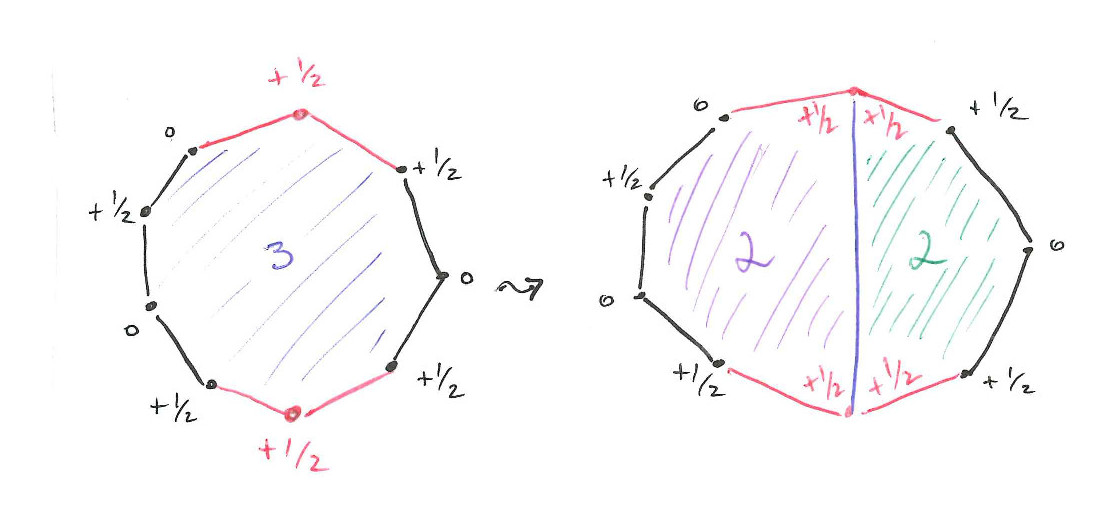
\includegraphics[width=5.5in]{figures/wedgenumblowup.jpg}
	\label{fig:wedgenumblowup}
\end{figure}
	
	\subsection{Building the Generic Piecewise--linear Map}
	\label{sub:genericplmap}
	This section comes to fruition with the definition of the piecewise--linear analog to a generic proper smooth map.
Let $T$ be a closed, orientable, edge--distinct 3--manifold triangulation.
We build a map $\pi':T'\to\C$ satisfying the following criteria:
\begin{enumerate}
	\item The space $T'$ is a solid polyhedral gluing whose boundary components are homeomorphic to $S^2$.
	\item Attaching 3--balls over the boundary components of $T'$ results in a complex homeomorphic to $T$.
	\item For any pair of edges $E$, $F$ in $T'$, if $\pi'(E)\cap\pi(F)=z$ is nonempty, then $z$ is not the intersection of any other pair of edges in $T'$.
	\item The wedge number of every edge of $T'$ is 0, 1, or 2.
\end{enumerate}
The first two conditions are met by modifying $T$ only through truncation and the blowing up of edges.
Condition 3 we obtain by requiring $\pi$ to be crossing distinct on $T$, and then modifying $T$ only in the controlled ways discussed in this section.
For condition 4, we blow up the appropriate edges.
The details are laid out in Algorithm \ref{alg:proj}, where we also obtain the 2--complex associated to $\pi'$ along the way.
We pass the results of Algorithm \ref{alg:proj} into the algorithms of Section \ref{sec:stein}

\begin{algorithm}[H]
	\caption{Building the piecewise--linear analogue to a generic proper smooth map}
	\label{alg:proj}
	\KwData{the closed, orientable, edge--distinct 3--manifold triangulation $T$}
	\KwResult{a map $\pi':T'\to\C$ satisying the above criteria, and the associated 2--complex $X'$}
	\Begin{
		$m\longleftarrow |T^0|$\;
		put an arbitrary order on $T^0$\;
		\ForEach{integer $k$ in $[1,m]$}{
			define $\pi(x_k)=e^{2\pi i \frac{k}{m}}$	
		}
		extend $\pi$ linearly as in Section \ref{sub:2complex}\;
		\ForEach{edge $E$ of $T$}{
			$w_E\longleftarrow$ result of Algorithm \ref{alg:computewedgenum}\;
			distribute $w_E$ across the tetrahedra containing $E$\;
		}
		truncate $T$ to $T'$ and $\pi$ to $\pi'$\;
		$X\longleftarrow$ result of Algorithm \ref{alg:neuter} on $\pi$\;
		\ForEach{internal edge $E'$ of $T'$}{
			\While{$w_E>2$}{
				$(\sigma^*,\tau^*)\longleftarrow$ result of Algorithm \ref{alg:wedgereduction}\;
				$\pi',T',T'^*,X'\longleftarrow$ result of blowing up $E'$ over $\sigma$ and $\tau$\;
				$w_E\longleftarrow w_E-1$\;
			}
		}
	}
\end{algorithm}

\section{The Stein Complex}
\label{sec:stein}
We enter this section with a piecewise linear analogue to the generic proper smooth map of Section \ref{sec:3bound4}, and focus on leaving it with a Stein complex to the map.
A generic proper smooth map already has a Stein complex that is described as a 2--complex, so this section is fairly straightforward and relatively light.
Only in Section \ref{sub:gleams} do we delve into complicated subject matter.
As we are running fully parallel with Section \ref{sec:3bound4}, the arguments can be easily compared.

Section \ref{sec:proj} ended by providing us with some explicit data structures.
These structures are taken as given in the following sections.
What we have to work with:
\begin{enumerate}
	\item A solid polyhedral gluing $T'$ that is homeomorphic to $T$ minus some 3--balls.
	\item A piecewise--linear map $\pi':T'\to\C$ analogous to a generic proper smooth map.
	\item A 2--complex $T'^*$ dual to $T'$.
	\item A 2--complex $X'$ generated by $\pi'$.
\end{enumerate}
We build the Stein complex for $\pi'$ in the order of increasing cells.
Our 2--complex $X'$ corresponds completely to the image of $T'$ through $\pi'$, so the factorization of $\pi'$ should yield a 2--complex very similar to $X'$.
The 2--complex $S$ built in this section is the only data structure passed to the algorithms of Section \ref{sec:4man}.

	\subsection{Stein as a CW--complex}
	\label{sub:zero}
	Our first task is to determine how to generate the vertices of the Stein complex $S$.
Each vertex $v$ of $X'$ yields a number of vertices in the Stein complex of $\pi'$, each of which map over $v$ it when we factor $\pi'$.
Here we have referred to $v$ as both the vertex of $X$ and the type 2 point in the image of $\pi'$ that the vertex corresponds to, and we do the same with the edges and 2--cells of $X'$.
According to the analysis in Section \ref{sec:3bound4}, a given vertex of $X'$ has at most two vertices in $S$ that will be difficult to find.
For $v$ a vertex of $X'$, introducing a vertex of $S$ over $v$ is based entirely on the behaviour of the circles that map over the regions incident to $v$.

In our first case, $v$ is an internal vertex.
There are four 2--cells $c_0,\dots,c_3$ of $X'$ that contain $v$ in their boundaries.
Put $C_i$ to be the collection of simplicial circles in $T'^*$ that project over $c_i$ as in the result of Algorithm \ref{alg:regularcircles}.
There are also four 1--cells $e_0,\dots,e_3$ where $e_i$ is the intersection of $c_i$ and $c_{i+1}$, indices computed modulo 4.
See Figure \ref{fig:vertexprime}.

An edge $E_0$ of $T'$ maps through $\pi'$ over $e_0$ and $e_3$, and $E_1$ maps over $e_1$ and $e_3$.
From Section \ref{sub:tridual} we know:
\begin{enumerate}
	\item $C_0\triangle \pd E_0^* = C_1$.
	\item $C_1\triangle \pd E_1^* = C_2$.
	\item $C_2\triangle \pd E_0^* = C_3$.
	\item $C_3\triangle \pd E_1^* = C_0$.
\end{enumerate} 
In the smooth case this is equivalent to finding cobordisms between sets of circles $C_i$ and $C_{i+1}$.
We say that an element $C_{i,k}$ of $C_i$ \emph{interacts} with an element $C_{i+1,j}$ of $C_{i+1}$ if $C_{i,k}\triangle C_{i+1,j}$ is either empty or exactly $\pd E_{\floor{i/2}}^*$.
Take the union of the $C_i's$ and partition it into subsets that such that any element of a subset interacts with at least one other element of that subset.
Call the set of subsets of $\bigcup_i C_i$ by $N(v)$ and call it the set of \emph{interactive elements} over $v$.
Every element of $N(v)$ adds a vertex to $S$ that is linked to the subset of $N(v)$ that spawned it.

In our second case, $v$ is a boundary vertex.
The analysis is exactly the same, except that there are only two 2--cells of $X'$ that are incident with $v$.
In $\C$, the last region incident to $v$ is $R_\infty$, so our analysis is simplified somewhat.
Otherwise, we perform the same steps as the internal case.

With the 0--cells of $S$ determined, we find 1--cells.
As with the vertices, the 1--cells of the Stein complex project over the 1--cells of $X'$.
Take $u$, $v$ vertices of $S$ adjacent over an edge $e$ of $X'$.
To find the associated edges of $S$, examine the sets of interactive elements over $u$ and $v$.
The shared circles within the elements of $N(u)$ and $N(v)$ tell us whether a pair of vertices are adjacent in $S$ as detailed in Algorithm \ref{alg:steinedges}.

Attaching the 2--cells is very similar to attaching the 1--cells.
A 2--cell of $S$ projects over a 2--cell $c$ of $X'$, and each 2--cell corresponds to a simplicial circle projecting through $\pi'$ over $c$.
The attachment is determined entirely by a cycle in the 1-skeleton of $S$, found in Algorithm \ref{alg:stein2cells}.

\begin{algorithm}[h]
	\caption{Finding vertices for the Stein complex}
	\label{alg:steinvertices}
	\KwData{a vertex $v$ of $X'$}
	\KwResult{the set $N(v)$ of sets of interacting circles near $v$}
	\Begin{
		$c_i\longleftarrow$ the 2--cells of $X'$ incident to $v$\;
		$C_i\longleftarrow$ the result of Algorithm \ref{alg:regularcircles} with input $c_i$\;
		$N(v)\longleftarrow\emptyset$\;
		\ForEach{circle $C_{0,k}$ in $C_0$}{
			$y\longleftarrow\{C_{0,k}\}$\;
			add each circle incident to $C_{0,k}$ to $y$\;
			add each circle incident to a circle incident to $C_{0,k}$ to $y$\;
			add $y$ to $N(v)$\;	
		}
	}
\end{algorithm}

\begin{algorithm}[h]
	\caption{Finding edges for the Stein complex}
	\label{alg:steinedges}
	\KwData{an edge $e=(u,v)$ of $X'$}
	\KwResult{the set $N(e)$ of pairs $(U,V)$ with $U\in N(u)$ and $V\in N(v)$ such that $U$ and $V$ are adjacent over an edge of $S$}
	\Begin{
		$N(u), N(v)\longleftarrow$ the results of Algorithm \ref{alg:steinvertices} with inputs $u$, $v$\;
		$N(e)\longleftarrow\emptyset$\;
		\ForEach{element $U$ of $N(u)$}{
			\ForEach{element $V$ of $N(v)$}{
				\If{$U\cap V\neq\emptyset$}{
					add $(U,V)$ to $N(e)$\;
				}
			}	
		}
	}
\end{algorithm}

\begin{algorithm}[h]
	\caption{Finding 2--cells for the Stein complex}
	\label{alg:stein2cells}
	\KwData{a 2--cell $c$ of $X'$ with $\{v_0,\dots,v_k\}=\pd c$}
	\KwResult{the set $N(c)$ of cycles $\{V_0,\dots,V_k\}$ where $V_i$ is in $N(v_i)$ such that a 2--cell is attached over $\{V_0,\dots,V_k\}$ in $S$}
	\Begin{
		$C\longleftarrow$ the result of Algorithm \ref{alg:regularcircles} with input $c$\;
		$N(v_i)\longleftarrow$ the result of Algorithm \ref{alg:steinvertices} with input $v_i$\;
		$N(c)\longleftarrow\emptyset$\;
		\ForEach{simplicial circle $C_j$ of $C$}{
			$N_j\longleftarrow\emptyset$\;
			\ForEach{integer $i$ in $[0,k]$}{
				\ForEach{element $V_i$ of $N(v_i)$}{
					\If{$C_j\in V_i$}{
						add $V_i$ to $N_j$\;
					}	
				}			
			}
			add $N_j$ to $N(c)$\;
		}
	}
\end{algorithm}

\begin{figure}
	\centering
	\captionsetup{justification=centering}
	\caption{A vertex in $X'$ and the circles that map over incident 2--cells}
	
\includegraphics[height=3cm]{figures/dummy.jpg}
	\label{fig:vertexprime}
\end{figure}

	\subsection{Building the Stein Complex}
	\label{sub:steinbuild}
	The preceding algorithms are now combined into Algorithm \ref{alg:steincomplex} to build our integer decorated Stein complex.

\begin{algorithm}
	\caption{Building the Stein complex}
	\label{alg:steincomplex}
	\KwData{the closed, orientable, edge--distinct 3--manifold triangulation $T$}
	\KwResult{an integer decorated Stein complex $S$}
	\Begin{
		$X'\longleftarrow$ the result of Algorithm \ref{alg:proj} with input $T$\;
		$S\longleftarrow\emptyset$\;
		\ForEach{vertex $v$ of $X'$}{
			\ForEach{element $V_i$ of $N(v)$}{
				add a vertex $v_i$ to $S$\;	
			}
		}
		\ForEach{edge $e=(u,v)$ of $X'$}{
			\ForEach{element $(U_i,V_j)$ of $N(e)$}{
				add an edge $(u_i,v_j)$ to $S$\;	
			}
		}
		\ForEach{2--cell $c$ of $X'$}{
			\ForEach{element $N_j$ of $N(c)$}{
				attach a 2--cell to $S$ over the cycle $N_j$\;
			}
		}
	}
\end{algorithm}

\section{The 4--manifold}
\label{sec:4man}
We leave Section \ref{sec:stein} with an integer decorated 2--complex that is taken to be the Stein complex for a map constructed in Section \ref{sec:proj} analogous to the generic proper smooth map of Section \ref{sec:3bound4}.
This complex is a set of instructions for building a cobordism of the pair $(M,\emptyset)$, shown in Section \ref{sec:3bound4}.
The steps to that construction were:
\begin{enumerate}
	\item Perform a 3--thickening of the 1--skeleton of the Stein complex.
	\item Locate a set of curves on the boundary that correspond to 
	\item
	
\end{enumerate}

	\subsection{The triangulated prism}
	\label{sub:nprism}
	The basic building block that we used in our 4--manifold reconstruction is the triangulated $n$--prism with identical walls.
Take $\sigma^n$ to be the standard $n$--simplex.
By $n$--prism, we mean the $n$--disc seen as $\sigma^{n-1}\times \II$ in Figure \ref{fig:nprism}.
The prism has canonical ``top'' and ``bottom'' faces which are $\sigma^{n-1}\times \{1\}$ and $\sigma^{n-1}\times \{-1\}$ respectively.
It also has $n$ identical ``walls'' which are $F^i(\sigma^{n-1})\times \II$ for each $i=0,\dots,n-1$.
The triangulation we construct for the $n$--prism is designed so that the walls have identical triangulations.
We do this so that we are able to perform an $n$--thickening of an $(n-1)$--dimensional triangulation.

\begin{figure}
	\centering
	\captionsetup{justification=centering}
	\caption{Sample 1--, 2--, and 3--prisms}
	
\includegraphics[height=3cm]{figures/dummy.jpg}
	\label{fig:nprism}
\end{figure}

If a pair of $\sigma^{n-1}$ are glued over a face, then we take those simplices to be the bottom faces of a pair of prisms.
We glue these prisms together over their corresponding walls.
This provides the two $\sigma^{n-1}$ with an $n$--dimensional thickening.
If we can do this to any pair of simplices, then we can do this to an entire triangulation, as in Algorithm \ref{alg:nthickening}

\begin{algorithm}[h]
	\caption{Thickening a triangulation}
	\label{alg:nthickening}
	\KwData{an $n$--dimensional triangulation $T$}
	\KwResult{an $(n+1)$--dimensional triangulation $H(T)$ that is the $(n+1)$--thickening of $T$}
	\Begin{
		$H(T)\longleftarrow \emptyset$\;
		\ForEach{$n$--simplex $\sigma$ of $T$}{
			add a triangulated $(n+1)$--prism $H(\sigma)$ to $T'$\;
		}
		\ForEach{face $F^i(\sigma)=F^j(\tau)$ over which a pair $\sigma$, $\tau$ of $n$--simplices are glued in $T$}{
			glue the $i\nth$ wall of $H(\sigma)$ to the $j\nth$ wall of $H(\tau)$\;			
		}
	}
\end{algorithm}

Considering $F^i(\sigma^{n-1})$ is an $(n-2)$--simplex, it is reasonable to build our prisms recursively.
The intuition is that we build an $(n-1)$--sphere whose walls are $(n-2)$--prisms, themselves with identical walls.
Then, we cone the $(n-1)$--sphere to make a triangulated $n$--prism.
The details are in Algorithm \ref{alg:nprism}, assuming the base case of the 1--prism being an edge.

\begin{algorithm}[h]
	\caption{Building a standard $n$--prism}
	\label{alg:nprism}
	\KwData{a positive integer $n$}
	\KwResult{$P^n$, a triangulated $n$--prism with identical walls}
	\Begin{
		\If{$n=1$}{
			$P^1=\II$\;
			
		} \Else {
			$\sigma_{-1}^n,\sigma_1^n\longleftarrow$ standard $n$--simplices\;
			$P^n\longleftarrow \sigma_{-1}^n\sqcup\sigma_1^n$\;
			$P_0^{n-1},P_1^{n-1},\dots,P_n^{n-1}\longleftarrow$ result of Algorithm \ref{alg:nprism} with input $n-1$\;
			
			\ForEach{$(n-1)$ prism $P_i^{n-1}$}{
				attach $\sigma_{-1}^{n-1}$ of $P_i^{n-1}$ to $F^i(\sigma_{-1}^n)$ of $\sigma_{-1}^n$ in $P^n$\;
				attach $\sigma_1^{n-1}$ of $P_i^{n-1}$ to $F^i(\sigma_1^n)$	of $\sigma_1^n$ in $P^n$\;
			}
			
			\ForEach{$n-2$ simplex $F^k(F^i(\sigma_{1}^n))=F^l(F^j(\sigma_{1}^n))$ of $\sigma_{1}^n$}{
				attach the wall of $P_i^{n-1}$ containing $F^k(F^i(\sigma_{1}^n))$ to the wall of $P_j^{n-1}$ containing $F^l(F^j(\sigma_{1}^n))$\;
			}
			$P^n\longleftarrow CP^n$, the cone on $P^n$\;
		}
	}
\end{algorithm}
	
	\subsection{Building a Handlebody}
	\label{sub:handlebody}
	The first construction in the proof of Theorem \ref{thm:3stein4} is a 3--handlebody regular neighbourhood of the 1--skeleton of our Stein complex $S$.
Put $G$ to be the 1--skeleton of $S$ and $A\subset G$ a maximal spanning tree.
We know that $G$ is a graph where, for any vertex $v$ of $G$, $\deg_G v$ is 3 if $v$ is boundary and 4 if it is interior.

We first triangulate the building blocks of Figure \ref{fig:3thickeningblocks} and display them in Figure \ref{fig:3thicktri}.
Each block in Figure \ref{fig:3thicktri} depicts one view of a triangulated 2--sphere.
The blocks have symmetry that should be clear, and the full triangulated block is found by taking the cone on the triangulated 2--sphere depicted.
Note that each edge block is actually a triangulated prism, and the only difference between the blocks is the set of marked boundary curves.
The proof of Theorem \ref{thm:3stein4} is procedural in its creation of handlebodies, and the details for the triangulated case are contained in Algorithm \ref{alg:4handlebody}.
In this section we use the notation laid out in the proof of Theorem \ref{thm:3stein4}, and we take $A\subset G$ to be fixed throughout.

The result of Algorithm \ref{alg:4handlebody} includes strips inside of solid tori $V$ used to compute 0--framing curves.
When the strip is an annulus, the curve is found as one of the boundary components of the annulus.
When it is a M\"obius strip, there is one boundary component $2\lambda$.
We take $2\Lambda$ halfway around its length to one full longitude of $V$, and perform one last positive half twist in order to get an actual 0--framing curve $\lambda$.
To be precise, the half twist is a curve $\gamma$ in the meridian direction of the boundary of $V$ connecting the endpoints of $\frac{1}{2}(2\lambda)$, and the positive direction is the anticlockwise direction determined by the $\II^2$ fibers over the boundary component of $U_S(G)$.

\begin{algorithm}
	\caption{Building the 4--handlebody of the 1--skeleton of the Stein complex}
	\label{alg:4handlebody}
	\KwData{a Stein complex $S$}
	\KwResult{a triangulated 4--manifold $A_4$ that is the 4--thickening of $U_S(G)$, a set of trianglated solid tori $\mathcal{V}$ in the boundary over which we will attach 2--handles, and a set of strips $\mathcal{C}$ in the boundary tori of $\mathcal{V}$ used to determine 0--framings as in the proof of Theorem \ref{thm:3stein4}}
	\Begin{
		$A_3,C\longleftarrow\emptyset$\;
		\ForEach{vertex $v$ of $A$}{
			add the triangulated vertex block $v_B$ associated to the type of vertex $v$ is in $S$ to $A$\;
			add the triangulated red curve in the boundary of $v_B$ depicted in Figure \ref{fig:3thicktri} to $C_A$\;
		}
		\ForEach{edge $e=(u,v)$ of $A$}{
			attach the triangulated edge block $e_B$ associated to the type of edge $e$ is in $S$ over the blocks $u_B$ and $v_B$\;
			add the triangulated red curve in the boundary of $e_B$ depicted in Figure \ref{fig:3thicktri} to $C_A$\;
			combine the curves in $C_A$ over identical boundaries\;
		}
		$A_4\longleftarrow$ result of Algorithm \ref{alg:nthickening} with input $A_3$\;
		$C_A\longleftarrow$ the inclusions of $C_A$ into the copies of $A_3$ at $A_3\times\{\pm1\}$ in $A_4$\;
		\ForEach{edge $e=(u,v)$ of $e(G)\setminus e(A)$}{
			$e_B\longleftarrow$ the triangulated edge block associated to the type of edge $e$ is in $S$\;
			$E_B\longleftarrow$ the result of Algorithm \ref{alg:nthickening} on $e_B$\;
			attach $E_B$ over the thickenings $U_B$ and $V_B$ of $u_B$ and $v_B$ in $A_4$ in the unique orientation preserving way\;
			add the pair of triangulated red curves from Figure \ref{fig:3thicktri} included into the copies of $e_B$ at $e_B\times\{\pm 1\}$ in $E_B$ to $C_A$\;
			combine the curves in $C_A$ over identical boundaries\;
		}
		$\mathcal{V},\mathcal{C}\longleftarrow\emptyset$\;
		\ForEach{curve $c$ of $C_A$}{
			$V\longleftarrow\emptyset$, to be the solid torus associated with $c$\;
			$C\longleftarrow\emptyset$, to be the strip in $V$ that determines 0--framing\;
			\ForEach{thickened 4--prism $P_i^4$ intersecting $c$ nontrivially}{
				$P_0^3,P_1^3\longleftarrow$ the identical walls of $P_i^4$, themselves 3--prisms, intersecting $c$ in an edge\;
				$P^2\longleftarrow$ the identical wall shared by $P_0^3,P_1^3$, itself a 2--prism\;
				add $P_0^3,P_1^3$ to $V$\;
				add $P^2$ to $C$\;				
			}
			combine the elements of $V$ over identical boundaries\;
			add $V$ to $\mathcal{V}$\;
			combine the elements of $C$ over identical boundaries\;
			add $C$ to $\mathcal{C}$\;
		}
	}	
\end{algorithm}

\begin{figure}
	\centering
	\captionsetup{justification=centering}
	\caption{The triangulated blocks used in the 3--thickening of the 1--skeleton of the Stein complex}
	
\includegraphics[height=3cm]{figures/dummy.jpg}
	\label{fig:3thicktri}
\end{figure}

	\subsection{Framing Coefficient Computation}
	\label{sub:gleams}
	Section \ref{sec:3bound4} ends with a discussion of framing coefficients with respect to a canonical 0--framing.
Take $V$ to be a solid torus of $M$ mapping through $\pi'$ to a disc $D$ in $\C$, itself existing as a shrunken region associated with a 2--cell $c$ of $S$ found in Section \ref{sub:zero}.
The zero section of $V$ as it sits in $T'$ can be represented by any of the 2--cells of $T'$ that intersect $V$ in a disc.
The simplicial circle representing the core of $V$ that projects through $\pi$ over $c$ is described by a dual cycle $c_V^*$ in the dual complex $T^*$, so any dual 1--cell of this description will suffice.
A section over $\pd D$ is realized as a closed walk over $c_V^*$, and the framing coefficient is the oriented number of times that the dual 1--cell representing $z(V)$ is traversed in this walk.

To describe a section over $\pd D$, we first describe a section over the portions of $\pd D$ that run parallel to edges in $X'$.
Let $e$ be such an edge, and $f$ its parallel strand in $D$.
A section over $e$ is a portion of an edge $E$ in $T'$.
An appropriate section over $f$, denoted $s(f)$, sits entirely inside of a single 3--cell $\sigma$ of $T'$ that contains $E$.
This is appropriate because of the piecewise--linear nature of $\pi$.

The section we construct will have the same oriented intersection number with any choice of zero section for $V$.
If $s(f)$ leaves $\sigma$, it leaves through a boundary 2--cell of $\sigma$.
If it does not travel at least once around $E$, then it is identical in our computations to the version of $s(f)$ that sits entirely inside of $\sigma$.
If it does travel around $E$, then recall that we may take as $z(V)$ \emph{any} 2--cell projecting over $D$.
Here, if a 2--cell incident to $E$ projects over $D$, then all of them must project over $D$, and no other 2--cell of $T'$ may project over $D$ in order to keep the oriented intersection number invariant.
In this case, $E$ forms a definite fold singularity so $s(f)$ can be isotoped through the 3--ball in $M$ associated to this type of singularity back to a position in which it sits entirely inside of $\sigma$.

We conclude that every intersection of $s(f)$ with $z(V)$ occurs near a vertex of $S$.
Referring back to the representative circle $c_V^*$ in the dual complex, we may associate $s(f)$ with a dual vertex $v_f^*$ in $c_V$.
The full section $s(\pd D)$ is then determined by how we walk between these vertices.

Ordering the edges of $\pd c$ and their parallel strands on $\pd D$, we investigate the arc used to connect $s(f_i)$ and $s(f_{i+1})$ in the section over $\pd D$.

\begin{algorithm}
	\caption{Computation of Framing Coefficients}
	\label{alg:gleams}
	\KwData{a 2--cell $c$ of the Stein complex $S$}
	\KwResult{the framing coefficient $n_c$ for $c$}
	\Begin{
		$f_0\longleftarrow\emptyset$, the 0--framing\;
		$R_c\longleftarrow$ the 2--cell of $X'$ over which $c$ projects\;
		$\Sigma\longleftarrow\emptyset$, the ordered vertices of $T'^*$ corresponding to the 0--framing near the edges of $c$\;
		\ForEach{edge $e_i$ in $\pd c=\{e_0,e_1,\dots,e_k,e_0\}$}{
			$E_i\longleftarrow$ the edge of $T'$ projecting over $e_i$\;
			$\sigma_i\longleftarrow$ a 3--cell $T'$ containing $E_i$ projecting over $R_c$\;
			add $\sigma_i^*$ to $\Sigma$\;
		}
		\ForEach{vertex $v_i$ in
			$\pd c=\{e_0=(v_0,v_1),e_1=(v_1,v_2),\dots,e_k=(v_k,v_0),e_0\}$
		}{
			
		}
	}	
\end{algorithm}
	
	\subsection{Building 2--handles}
	\label{sub:2handles}
	This algorithm takes as input:
\begin{enumerate}
  \item a triangulated open solid torus $V$ which is a subtriangulation of a triangulated 3--manifold $M$, itself the boundary of a triangulated 4--manifold $W$,
  \item a triangulated longitude of $V$ represented by a curve $z$ in the boundary of $V$ which is defined as the 0--framing of the core of $V$ in $M$,
  \item a triangulated longitude of $V$ represented by a curve $N$ in the boundary of $V$ which intersects $z$ only at vertices in exactly $n$ points.
\end{enumerate}
This algorithm gives as output the manifold $W\cup_\varphi h$, where $h$ is a 2--handle which is attached to $W$ over the attaching region $V$ and whose attaching sphere has framing datum associated with the element $n$ of $\pi_1(O(2))$ with respect to the 0--framing of $z$.

First, we detail the completion of an open solid torus into a 4--ball.
Let $V$ be a triangulated open solid torus, and $\lambda$ a triangulated longitude of $V$.
Then $\pd V |\lambda$ is the boundary torus of $V$ cut along the curve $\lambda$.
This object is an annulus $A$ whose boundary circle have the same triangulation $C$.
The cone $C(A)$ on $A$ is not a manifold, but the only place at which $C(A)$ is degenerate is the coning point.
We fix this by letting $B$ be the 3--ball triangulated by a number of tetrahedron equal to the number of edges is $C$, each of which share a common edge $e$.
Then $\lk(e)$ in $B$ is $C$, and the boundary of $B$ is made of two triangulated discs which are equal to the cone on $C$.
We attach $B$ to $C(A)$ in the obvious way.
The result is the open solid torus $U$ which has boundary whose triangulation is equal to the triangulation of the boundary of $V$.
The curve $\lambda$ of $U$ is a meridian of $U$, so it bounds a disc inside of $U$.
Gluing $U$ to $V$ along their identical boundaries produces a 3--sphere $sph(V,\lambda)=U\cup V$.
Then the 0--framing of the core of $V$ in $sph(V,\lambda)$ is given by $\lambda$, as $V$ is unknotted in $sph(V,\lambda)$, and $\lambda$ bounds a Seifert surface which is a disc in $sph(V,\lambda)$.
The cone on $sph(V,\lambda)$, $C(sph(V,\lambda))$, is a 4--ball whose prescribed 2--handle structure is defined by a core, which is the Seifert surface disc that $\lambda$ bounds, and attaching region $V$.
Then we denote $C(sph(V,\lambda))$ by $cmpl(V,\lambda)$ and call this object the \emph{4--dimensional 2--handle of the pair $(V,\lambda)$}.

With the input data, we attach the 4--dimensional 2--handle $cmpl(V,N)$ to $M$ via the attaching map that identifies the copy of $V$ in $cmpl(V,N)$ with the copy $V$ in $M$.

	
	\subsection{Building the 4--manifold}
	\label{sub:final}
	We tie the algorithms of Section \ref{sec:4man} together into Algorithm \ref{alg:4manifold}.

\begin{algorithm}
	\caption{Building a 4--manifold}
	\label{alg:4manifold}
	\KwData{the closed, orientable, edge--distinct 3--manifold triangulation $T$}
	\KwResult{a triangulated 4--manifold $W$ with boundary triangulation homeomorphic to the closed orientable 3--manifold $M$ whose triangulation was taken as input to Algorithm \ref{alg:proj}}
	\Begin{
		$S\longleftarrow$ the result of Algorithm \ref{alg:steincomplex} with input $T$\;
		$W,\mathcal{V},\mathcal{C}\longleftarrow$ the result of Algorithm \ref{alg:4handlebody} with input $S$\;
		$\Lambda\longleftarrow$ the set of pairs $(V,\lambda)$ with $V$ from $\mathcal{V}$ and $\lambda$ the 0--framing of $V$\;
		\ForEach{pair $(V,\lambda)$ of $\Lambda$}{
			$n\longleftarrow$ the framing coefficient of the 2--cell of $S$ corresponding to $V$\;
			$W\longleftarrow$ the result of subdividing $V$ to a triangulated solid torus $V'$ for which a curve $\lambda^n$ as described in Section \ref{sub:2handles} exists\;
			$\lambda'\longleftarrow$ the subdivision of $\lambda$ from the previous line\;
			$H^4\longleftarrow$ the result of Algorithm \ref{alg:2handle} with input $V'$,$\lambda'$,$n$\;
			$W\longleftarrow$ the result of gluing $H^4$ to $W$ over $V'$\;
		}
	}
\end{algorithm}



\chapter{Conclusion}




%\appendix
%\label{app:alg}




\chapter{Algorithms from Chapter 4}
\begin{algorithm}
  \label{alg:a1over}
    \KwIn{Edge-distinct triangulation $T$ of the 3--manifold $M$}
    \KwOut{Planar graph $G$, polyhedral 3--complex $T'$,  with spherical boundary components}
     
      Build a PL projection $\pi:T\to\RR$\;
      Obtain a planar graph $G$ from the combinatorics of $\pi$\; 
      Collect regional and edge information\;
      Return ($G$,++)
      
    \caption{Obtaining a planar graph with additional data}
\end{algorithm}


\begin{algorithm}
  \KwIn{Edge distinct 3--manifold triangulation T}
  \KwOut{Piecewise--linear projection $\pi:T\to \C$}

  Order the vertices of $T$ and label them $v_i$, starting at $v_0$;
  Let $k$ be the smallest odd number at least as large as $|T^0|$;
  \For{$i$ from $0$ to $|T^0|$}
  {
    Define $\pi(v_i)=e^{2\pi i/k}$;
  }
  \For{Edges $e=v_i v_j$ in $T^1$}
  {
    Define $\pi()$
  }

\end{algorithm}


\begin{algorithm}
  \KwIn{Vertex $v$ from $V(G)$ with degree $d_G(v)\geq 2$ from a planar graph $G$}
  \KwOut{List of chordless cycles containing $v$}

  Initiate empty list $L(v)$

  \Repeat{$d_G(v)\leq 1$}
  {
    Choose any edge $e$ adjacent to $v$;
  }

\end{algorithm}


\begin{algorithm}
    \KwIn{Planar graph $G$}
    \KwOut{List of chordless cycles $L$}
    
    Initiate empty list $L$;
    
    \Repeat{$V(G)$ is empty}
    {
      \Repeat{$d_G(v)\geq 2$ For each $v$ in $V(G)$}
      {
        Delete each vertex of degree at most 1;
      }
      Let $v$ be an arbitrary vertex of $G$;
    }
\end{algorithm}


\chapter{Algorithms from Chapter 5}
\begin{algorithm}
  \label{alg:a2over}
  \SetKwInOut{Input}{Input}
    \SetKwInOut{Output}{Output}

    \Input{Planar graph ($G$,++)}
    \Output{Shadow $(S,\glm)$}
      Construct a region in $S$ for every OST pulled back to by a region of $G$\;
      Connect regions of $S$ according to instructions from the edges of $G$\;
      Fill holes of $S$ according to instructions from the edges of $G$\;
      Mark external boundary as false\;
      Compute gleams $\glm$ of regions of $S$\;
      Return $(S,\glm)$\;
    \caption{Building a shadow}
\end{algorithm}


\chapter{Algorithms from Chapter 6}




\bibliography{mybib}{}
\bibliographystyle{plain}



\end{document}
